% chktex-file 44
\renewcommand{\thesection}{\Alph{section}}
\section{External Interface Requirements}
\subsection{User Interfaces}\label{sec:UserInterfaces}
As the users of the platform include students, companies, and universities, the user interface is designed to facilitate interaction with 
the platform and meet their needs. For instance, many students may be unfamiliar with the internship search process and may lack experience
in finding job opportunities, so the user interface should be simple and intuitive to use.

In the following section, we describe the drafts of the principal Graphical User Interfaces (GUIs). These will be further detailed
using refined mockups in the Design Document.
\begin{itemize}
    \item \textbf{Welcome page:} The welcome page is the first page users see when they open the platform. It contains the platform's logo 
    and a brief description of its purpose. On this page, users can log in using their credentials or create an account if they are new
    to Students\&Companies.
    
    \item \textbf{Registration Page:} In the registration page, users will first be asked to select their user type (student, company, or
     university). Based on the selected user type, the corresponding registration form will be displayed, and users will be prompted to 
     provide the necessary information to create an account. In addition to common data such as name, email, and password, users will
     need to provide additional information based on their user type. For example, students will be asked to personalize their profiles by 
     adding details such as their interests, skills, CV, university and a short description of themselves, while companies will be 
     asked their EIN number, etc.
    
    \item \textbf{Notification Page:} It will display various types of notifications received from the platform. For example, students will
    see notifications about updates on their application status, companies will receive notifications about the student’s decision, and 
    universities will be notified about new student registrations on the platform.

    \item \textbf{Side Menu:} The side menu is a navigation menu that provides access to the main sections of the platform and depends on the
    user's type. It will be displayed on the left side of the screen, with different sections available based on the user type (further explanation 
    below).

    \item \textbf{Header Bar:} The header bar is displayed at the top of the screen and includes the platform's logo, a Side Menu icon, a chat 
    icon, a notification icon, and the user's profile icon. It remains visible on all pages once the user has logged in.

    \item \textbf{Chat Interface:} The chat interface is accessible from the header bar. It allows students and companies to communicate with 
    each other in real-time. They can view a list of available chats, send and receive messages, and access their chat history.

    \item \textbf{Profile Page:} On this page, users can view other users' public information. If they own the profile, they can edit their data 
    as needed (by filling the fields in the "Edit Profile" page). Specifically, students can update their CV by accessing this page.

    \item \textbf{Search page:} This page contains a search bar and displays the results based on the user's search. For example, a student
    can search for internships, and the platform will return a list of results based on the student's input. 
    
    \item \textbf{Internship evaluation page:} This page is used by both students and companies to evaluate internship performance. Both 
    parties can provide feedback or complaints during the internship. At the end, to complete the evaluation process, they must leave
    final comments and rate the internship.

    \item \textbf{Internship details page:} This page displays detailed information about a specific internship. For example, all users can
    view the internship's description, requirements, and application deadline.

\end{itemize}

Since the platform is designed for three types of users, the specialized interfaces for each of them are described in further detail
below, considering their characteristics.
\begin{itemize}
    \item \textbf{Student Interfaces:}
    \begin{itemize}
        \item \textbf{Student Dashboard:} This is the home page that appears once the student logs in. On this page, the student gets an 
        overview of all the main functionalities they can access. The dashboard consists of:

        1. Search Bar with Filter Command: Allows to perform keyword searching.
        
        2. Overview of Recommended Internships: Displays job search keywords and internships recommended by the platform's algorithm.
        
        3. My Applications: Provides an overview of the student's applications' status.
        
        4. My Internships: Displays a record of the internships the student has applied for in the past, including the internship they 
        are currently doing if exist.

        \item \textbf{Student Side Menu:} For students, the side menu will include sections such as Search Internships, Dashboard, 
        My Applications and My Internships.

        \item \textbf{My applications:} The student can track the status of their applications and view the details of the internships 
        they have applied for. Through this interface, the student can also receive information related to the selection process, such 
        as the interview date, the interview result, and the final decision of the company. Additionally, the student can filter their 
        applications based on their status, such as ``waiting''.

        \item \textbf{My Internships:} The student can view the internships they have participated in so far, along with the evaluations 
        related to their experiences. If the student is currently participating to an internship, it will be displayed at the top. The 
        page also allows the student to access the Internship Evaluation page, where they can leave comments or notes about a specific internship.

    \end{itemize}
    \item \textbf{Company Interfaces:} 
    \begin{itemize}
        \item \textbf{Company Dashboard:} It's the home page that appears once the company logs in. On this page, the company gets an overview of 
        all the main functionalities they can access. The dashboard consists of:

        1. Search Bar with Filter Command: Allows to perform keyword searching.
        
        2. Overview of recommended Student Profiles: Displays student profiles recommended by the platform's matching algorithm for the internship 
        announcements that have been published by the company.
        
        3. Internship Announcements: A list of internship announcements the company has published, along with the number of the applications
        received.

        \item \textbf{Company Side Menu:} The side menu of companies includes sections such as Search Profile, Dashboard, Publish Internship,
        and Internships Management.
        
       \item \textbf{Publish Internship Page:} This is the main functionality of the company interface. On this page, the company can 
       create a new internship announcement and post it on the platform. The company is required to enter the necessary information, 
       following the guidelines provided by the platform.

        \item \textbf{Internship management page:} This page is divided into several sections: one for internship announcements that have 
        been published but are still in the publication phase, one for internships in the selection phase, one for internships currently 
        in progress, and one for closed internships. From this interface, the company can manage internships of all phases.
    \end{itemize}

    \item \textbf{University Interfaces:} 
    \begin{itemize}
        \item \textbf{University Dashboard:} The university dashboard displays a list of students and their associated activities. 
        The university can view the list of students registered on the platform and select a student to see detailed information about 
        their profile, activities, and internships they are currently doing or have completed in the past.

        \item \textbf{University Side Menu:} For universities, the side menu will include sections such as Search Profile and Dashboard.
    \end{itemize}
\end{itemize}


\subsection{Hardware Interfaces}
Students\&Companies is a web-based platform, so it can be accessed from any device with an internet connection. The platform is
compatible with all modern web browsers. It is designed to be responsive and work on different screen sizes, including desktops, 
laptops, tablets, and smartphones. \\
The system will be hosted on multiple server that meet the requirements for web hosting. They will be responsible for the platform's 
backend processes, such as the recommendation algorithm, the data collection and storing and the statistical analyses.


\subsection{Software Interfaces}
S\&C will interact with an emailing system to confirm the registration of new users. \\
It will also integrate various APIs to provide additional functionalities, for instance an API for implementing statistical analyses 
based on collected data that will be used to improve the recommendation algorithm. Another example would be an API to interact with
the database in order to store and retrieve information.


\subsection{Communication Interfaces}
The system will use HTTPS to ensure secure communication between the client and the server. The platform will also use WebSockets to
enable real-time communication between users, that is required by functionalities such as the chat. Since the platform is designed to be a 
RESTful web application, it will use JSON as the data exchange format between the client and the server. \\
To interact with the mailing system, the platform will use SMTP protocol.


\section{Functional Requirements}
The functional requirements that the platform must meet to achieve the user's needs are described below.
\subsection{Functional Requirements}
[R1] S\&C allows unregistered Users to sign up

[R2] S\&C allows registered Users to login	

[R3] S\&C allows STs to upload their CV in their profile section

[R4] S\&C allows STs to search for internships

[R5] S\&C allows COs to create internships by compiling all the information

[R6] S\&C allows COs to set a deadline for submitting the application to an internship

[R7] S\&C allows COs to publish internships

[R8] S\&C should notify STs when they are selected by the CO for the interview process

[R9] S\&C should notify STs when a CO is interested in their profile

[R10] S\&C should notify STs when he is successfully selected for a position

[R11] S\&C should notify STs when a CO rejects their application

[R12] S\&C should notify UNIs when their students start an internship

[R13] S\&C should notify STs when an internship available matches their interest.

[R14] S\&C should notify COs when the deadline for a published internship has expired

[R15] S\&C should notify COs when the candidate accepts the position

[R16] S\&C should notify COs when the candidate refuses the position

[R17] S\&C should notify COs and STs when a new chat message is available

[R18] S\&C should notify COs when a ST with a CV that corresponds to their needs is available

[R19] S\&C should be able to analyze the User’s data to provide the recommendations to both STs and COs

[R20] S\&C allows STs to submit their application for an internship	

[R21] S\&C allows STs to visualize information about a published internship

[R22] S\&C allows COs to view the list of all applications that were submitted for a specific internship

[R23] S\&C allows COs to record STs selection outcomes

[R24] S\&C allows COs to create forms to submit to candidates for the interview process

[R25] S\&C allows candidates to respond to the received forms

[R26] S\&C allows COs to visualize the responses of the candidates who have replied to the forms

[R27] S\&C allows COs to record the results of the interview

[R28] S\&C allows STs to check the status of their applications

[R29] S\&C allows STs to accept or reject the offer after receiving the interview results

[R30] S\&C allows STs and COs to write feedback and complaints relating to the internship experience

[R31] S\&C allows Users to view feedback and complaints relating to the internship experience

[R32] S\&C allows STs and COs to exchange information using the chat, only if the ST is participating or has participated in an internship offered by the company

[R33] S\&C allows UNIs to check the status of the internship records of their students.

[R34] S\&C allows UNIs to access the list of all the enrolled STs that are registered on the platform

[R35] S\&C allows Users to visualize the own and other users' profiles

[R36] S\&C allows Users to modify their own profile data

[R37] S\&C should notify UNIs when their students register on the platform


\subsection{Requirement Mapping}
In the following table, represent the mapping between the goals, requirements and domain assumptions. The requirements are
mapped to the goals they contribute to, and the domain assumptions they depend on.
\begin{center}
    \begin{tabular}{|>{\columncolor{bluepoli!40}}c|p{20em}|p{13em}|}
        \hline
        \textbf{Goal} & \textbf{Requirement} & \textbf{Domain Assumption} \\
        \hline
        G1  & R1, R2    & A1, A2, A5, A6, A7 \\
        G2  & R3, R36   & A3, A5, A6, A7 \\
        G3  & R4, R21   & A6, A7, A10 \\
        G4  & R5, R6, R7 & A4, A6, A7, A8, A10 \\
        G5  & R8, R9, R10, R11, R12, R13, R14, R15, R16, R17, R18, R37 & A6, A7 \\
        G6  & R13, R18, R19 & A3, A6, A7 \\
        G7  & R20, R21 & A3, A6, A7, A9, A10, A11 \\
        G8  & R22, R23, R24 & A4, A6, A7, A11 \\
        G9  & R25 & A6, A7 \\
        G10 & R26, R27 & A4, A6, A7 \\
        G11 & R28, R29 & A6, A7 \\
        G12 & R30, R31, R37 & A6, A7, A10, A11 \\
        G13 & R32 & A6, A7, A10, A11 \\
        G14 & R33, R34, R35 & A6, A7 \\
        \hline
    \end{tabular}
\end{center}

\begin{center}
    \begin{tabular}{|p{37em}|}
        \rowcolor{bluepoli!40} % comment this line to remove the color
        \hline
        \textbf{[G1] All unregistered users must be able to create an account on the platform using their
        specific email address and log in to the platform.} \\
        % -------------------------------------------------------
        \rowcolor{bluepoli!15}
        \textbf{[R1] S\&C allows unregistered user to sign up}\\
        \rowcolor{bluepoli!15}
        \textbf{[R2] S\&C allows registered Users to login} \\
        % -------------------------------------------------------
        \textbf{[A1] The university of the student who want to register on the platform must be listed in the platform's database. If the university is not listed, the student
        will not be able to complete the registration process.} \\
        \textbf{[A2] All users who want to use the platform must have an email address and necessary information to verify their identity.} \\
        \textbf{[A5] The platform will be able to communicate correctly with email servers to verify users' identity.}\\
        \textbf{[A6] Users have a stable internet connection to access the platform.}\\
        \textbf{[A7] The users of the platform must have a device that supports the platform's features.}\\
        \hline
    \end{tabular}
\end{center}

\begin{center}
    \begin{tabular}{|p{37em}|}
        \rowcolor{bluepoli!40} % comment this line to remove the color
        \hline
        \textbf{[G2] Students must be able to upload their CVs on the platform.} \\
        % -------------------------------------------------------
        \rowcolor{bluepoli!15}
        \textbf{[R3] S\&C allows STs to upload their CV in their profile section} \\
        \rowcolor{bluepoli!15}
        \textbf{[R36] S\&C allows Users to modify their own profile data} \\
        % -------------------------------------------------------
        \textbf{[A3] All students should have a CV that contains all the necessary information and details about their experience.} \\
        \textbf{[A5] The platform will be able to communicate correctly with email servers to verify users’ identity.}\\
        \textbf{[A6] Users have a stable internet connection to access the platform.}\\
        \textbf{[A7] The users of the platform must have a device that supports the platform's features.}\\
        \hline
    \end{tabular}
\end{center}

\begin{center}
    \begin{tabular}{|p{37em}|}
        \rowcolor{bluepoli!40} % comment this line to remove the color
        \hline
        \textbf{[G3] Students must be able to search for available internship offers on the platform.} \\
        % -------------------------------------------------------
        \rowcolor{bluepoli!15}
        \textbf{[R4] S\&C allows STs to search for internships} \\
        \rowcolor{bluepoli!15}
        \textbf{[R21] S\&C allows STs to visualize information about a published internship.} \\
        % -------------------------------------------------------
        \textbf{[A6] Users have a stable internet connection to access the platform.}\\
        \textbf{[A7] The users of the platform must have a device that supports the platform's features.}\\
        \textbf{[A10] Companies who have an account on the platform will eventually publish internships.}\\
        \hline
    \end{tabular}
\end{center}

\begin{center}
    \begin{tabular}{|p{37em}|}
        \rowcolor{bluepoli!40} % comment this line to remove the color
        \hline
        \textbf{[G4] Companies must be able to publish internship offers on the platform.} \\
        % -------------------------------------------------------
        \rowcolor{bluepoli!15}
        \textbf{[R5] S\&C allows COs to create internships by compiling all the information.} \\
        \rowcolor{bluepoli!15}
        \textbf{[R6] S\&C allows COs to set a deadline for submitting the application to an internship.}\\
        \rowcolor{bluepoli!15}
        \textbf{[R7] S\&C allows allows COs to publish internships.}\\
        % -------------------------------------------------------
        \textbf{[A4] Every department of a company has a unique email address that identify it.}\\
        \textbf{[A6] Users have a stable internet connection to access the platform.}\\
        \textbf{[A7] The users of the platform must have a device that supports the platform's features.}\\
        \textbf{[A8] The companies do not publish the same internship announcement more than once before the application deadline.}\\
        \textbf{[A10] Companies who have an account on the platform will eventually publish internships.}\\
        \hline
    \end{tabular}
\end{center}

\begin{center}
    \begin{tabular}{|p{37em}|}
        \rowcolor{bluepoli!40} % comment this line to remove the color
        \hline
        \textbf{[G5] Users must receive notifications about relevant events.} \\
        % -------------------------------------------------------
        \rowcolor{bluepoli!15}
        \textbf{[R8] S\&C should notify STs when they are selected by the CO for the interview process.} \\
        \rowcolor{bluepoli!15}
        \textbf{[R9] S\&C should notify STs when a CO is interested in their profile.} \\
        \rowcolor{bluepoli!15}
        \textbf{[R10] S\&C should notify STs when he is successfully selected for a position.} \\
        \rowcolor{bluepoli!15}
        \textbf{[R11] S\&C should notify STs when a CO rejects their application.} \\
        \rowcolor{bluepoli!15}
        \textbf{[R12] S\&C should notify UNIs when their students start an internship.} \\
        \rowcolor{bluepoli!15}
        \textbf{[R13] S\&C should notify STs when an internship who matches their interest is available.} \\
        \rowcolor{bluepoli!15}
        \textbf{[R14] S\&C should notify COs when the deadline for a published internship has expired.} \\
        \rowcolor{bluepoli!15}
        \textbf{[R15] S\&C should notify COs when the candidate accepts the position.} \\
        \rowcolor{bluepoli!15}
        \textbf{[R16] S\&C should notify COs when the candidate refuses the position.} \\
        \rowcolor{bluepoli!15}
        \textbf{[R17] S\&C should notify COs when a new chat message is available.} \\
        \rowcolor{bluepoli!15}
        \textbf{[R18] S\&C should notify COs when a ST with a CV that corresponds to their needs is available.} \\
        \rowcolor{bluepoli!15}
        \textbf{[R37] S\&C should notify UNIs when their students register on the platform.} \\
        % -------------------------------------------------------
        \textbf{[A6] Users have a stable internet connection to access the platform.}\\
        \textbf{[A7] The users of the platform must have a device that supports the platform's features.}\\
        \hline
    \end{tabular}
\end{center}

\begin{center}
    \begin{tabular}{|p{37em}|}
        \rowcolor{bluepoli!40} % comment this line to remove the color
        \hline
        \textbf{[G6] Students and Companies must receive recommendations based on statistical analyses.} \\
        % -------------------------------------------------------
        \rowcolor{bluepoli!15}
        \textbf{[R13] S\&C should notify STs when an internship who matches their interest is available.} \\
        \rowcolor{bluepoli!15}
        \textbf{[R18] S\&C should notify COs when a ST with a CV that corresponds to their needs is available.} \\
        \rowcolor{bluepoli!15}
        \textbf{[R19] S\&C should be able to analyze the User’s data to provide the recommendations to both STs and COs.} \\
        % -------------------------------------------------------
        \textbf{[A3] All students should have a CV that contains all the necessary information and details about their experience.} \\
        \textbf{[A6] Users have a stable internet connection to access the platform.}\\
        \textbf{[A7] The users of the platform must have a device that supports the platform's features.}\\
        \hline
    \end{tabular}
\end{center}

\begin{center}
    \begin{tabular}{|p{37em}|}
        \rowcolor{bluepoli!40} % comment this line to remove the color
        \hline
        \textbf{[G7] Students must be able to proactively apply for internships, before the submission deadline.} \\
        % -------------------------------------------------------
        \rowcolor{bluepoli!15}
        \textbf{[R20] S\&C allows STs to submit their application for an internship.} \\
        \rowcolor{bluepoli!15}
        \textbf{[R21] S\&C allows STs to visualize information about a published internship.} \\
        % -------------------------------------------------------
        \textbf{[A3] All students should have a CV that contains all the necessary information and details about their experience.} \\
        \textbf{[A6] Users have a stable internet connection to access the platform.}\\
        \textbf{[A7] The users of the platform must have a device that supports the platform's features.}\\
        \textbf{[A9] The student do not apply for the internship if she/he has already accepted offer which starts in the same period.}\\
        \textbf{[A10] Companies who have an account on the platform will eventually publish internships.}\\
        \textbf{[A11] Students who have an account on the platform will eventually apply for internships.}\\
        \hline
    \end{tabular}
\end{center}

\begin{center}
    \begin{tabular}{|p{37em}|}
        \rowcolor{bluepoli!40} % comment this line to remove the color
        \hline
        \textbf{[G8] Companies must be able to set up the interview process.} \\
        % -------------------------------------------------------
        \rowcolor{bluepoli!15}
        \textbf{[R22] S\&C allows COs to view the list of all applications that were submitted for a specific internship.} \\
        \rowcolor{bluepoli!15}
        \textbf{[R23] S\&C allows COs to record STs selection outcomes.} \\
        \rowcolor{bluepoli!15}
        \textbf{[R24] S\&C allows COs to create forms to submit to candidates for the interview process.} \\
        % -------------------------------------------------------
        \textbf{[A4] Every department of a company has a unique email address that identify it.}\\
        \textbf{[A6] Users have a stable internet connection to access the platform.}\\
        \textbf{[A7] The users of the platform must have a device that supports the platform's features.}\\
        \textbf{[A11] Students who have an account on the platform will eventually apply for internships.}\\
        \hline
    \end{tabular}
\end{center}

\begin{center}
    \begin{tabular}{|p{37em}|}
        \rowcolor{bluepoli!40} % comment this line to remove the color
        \hline
        \textbf{[G9] During the interview process, students must be able to respond to the company's questions through questionnaires.} \\
        % -------------------------------------------------------
        \rowcolor{bluepoli!15}
        \textbf{[R25] S\&C allows candidates to respond to the received forms.} \\
        % -------------------------------------------------------
        \textbf{[A6] Users have a stable internet connection to access the platform.}\\
        \textbf{[A7] The users of the platform must have a device that supports the platform's features.}\\
        \hline
    \end{tabular}
\end{center}

\begin{center}
    \begin{tabular}{|p{37em}|}
        \rowcolor{bluepoli!40} % comment this line to remove the color
        \hline
        \textbf{[G10] Companies must be able to send the results of the interviews to the students.} \\
        % -------------------------------------------------------
        \rowcolor{bluepoli!15}        
        \textbf{[R26] S\&C allows COs to visualize the responses of the candidates who have replied to the forms.} \\
        \rowcolor{bluepoli!15}
        \textbf{[R27] S\&C allows COs to record the results of the interview.} \\
        % -------------------------------------------------------
        \textbf{[A4] Every department of a company has a unique email address that identify it.}\\
        \textbf{[A6] Users have a stable internet connection to access the platform.}\\
        \textbf{[A7] The users of the platform must have a device that supports the platform's features.}\\

        \hline
    \end{tabular}
\end{center}

\begin{center}
    \begin{tabular}{|p{37em}|}
        \rowcolor{bluepoli!40} % comment this line to remove the color
        \hline
        \textbf{[G11] Students must be able to accept or reject the offer after receiving the interview results.} \\
        % -------------------------------------------------------
        \rowcolor{bluepoli!15}
        \textbf{[R28] S\&C allows STs to check the status of their applications.} \\
        \rowcolor{bluepoli!15}
        \textbf{[R29] S\&C allows STs to accept or reject the offer after receiving the interview results.} \\
        % -------------------------------------------------------
        \textbf{[A6] Users have a stable internet connection to access the platform.}\\
        \textbf{[A7] The users of the platform must have a device that supports the platform's features.}\\
        \hline
    \end{tabular}
\end{center}

\begin{center}
    \begin{tabular}{|p{37em}|}
        \rowcolor{bluepoli!40} % comment this line to remove the color
        \hline
        \textbf{[G12] Students and companies must be able to write feedback regarding their internship experiences.} \\
        % -------------------------------------------------------
        \rowcolor{bluepoli!15}
        \textbf{[R30] S\&C allows STs and COs to write feedback and complaints relating to the internship experience.} \\
        \rowcolor{bluepoli!15}
        \textbf{[R31] S\&C allows Users to view feedback and complaints relating to the internship experience.} \\
        \rowcolor{bluepoli!15}
        \textbf{[R37] S\&C should notify UNIs when their students register on the platform.} \\
        % -------------------------------------------------------
        \textbf{[A6] Users have a stable internet connection to access the platform.}\\
        \textbf{[A7] The users of the platform must have a device that supports the platform's features.}\\
        \textbf{[A10] Companies who have an account on the platform will eventually publish internships.}\\
        \textbf{[A11] Students who have an account on the platform will eventually apply for internships.}\\
        \hline
    \end{tabular}
\end{center}

\begin{center}
    \begin{tabular}{|p{37em}|}
        \rowcolor{bluepoli!40} % comment this line to remove the color
        \hline
        \textbf{[G13] Students and companies must be able to communicate with each other during internship process.} \\
        % -------------------------------------------------------
        \rowcolor{bluepoli!15}
        \textbf{[R32] S\&C allows STs and COs to exchange information using the chat, only if the ST is participating 
        or has participated in an internship offered by the company.} \\
        % -------------------------------------------------------
        \textbf{[A6] Users have a stable internet connection to access the platform.}\\
        \textbf{[A7] The users of the platform must have a device that supports the platform's features.}\\
        \textbf{[A10] Companies who have an account on the platform will eventually publish internships.}\\
        \textbf{[A11] Students who have an account on the platform will eventually apply for internships.}\\
        \hline
    \end{tabular}
\end{center}

\begin{center}
    \begin{tabular}{|p{37em}|}
        \rowcolor{bluepoli!40} % comment this line to remove the color
        \hline
        \textbf{[G14] Universities must be able to monitor the internship process of their students.} \\
        % -------------------------------------------------------
        \rowcolor{bluepoli!15}
        \textbf{[R33] S\&C allows UNIs to check the status of the internship records of their students.} \\
        \rowcolor{bluepoli!15}
        \textbf{[R34] S\&C allows UNIs to access the list of all the enrolled STs that are registered on the platform.} \\
        \rowcolor{bluepoli!15}
        \textbf{[R35] S\&C allows Users to visualize the own and other users' profiles.} \\
        % -------------------------------------------------------
        \textbf{[A6] Users have a stable internet connection to access the platform.}\\
        \textbf{[A7] The users of the platform must have a device that supports the platform's features.}\\
        \hline
    \end{tabular}
\end{center}

\subsection{Use Case Diagram}
In following section, the use case diagrams, the use cases description and the sequence diagrams are presented to describe 
the interaction between the users and the platform in a more detailed way.

\subsubsection{Use Case Diagrams}
The use case is divided into three main actors: Students, Companies and Universities. Each actor has a set of use cases that
describe the functionalities he can access on S\&C.
\begin{figure}[H]
    \centering
    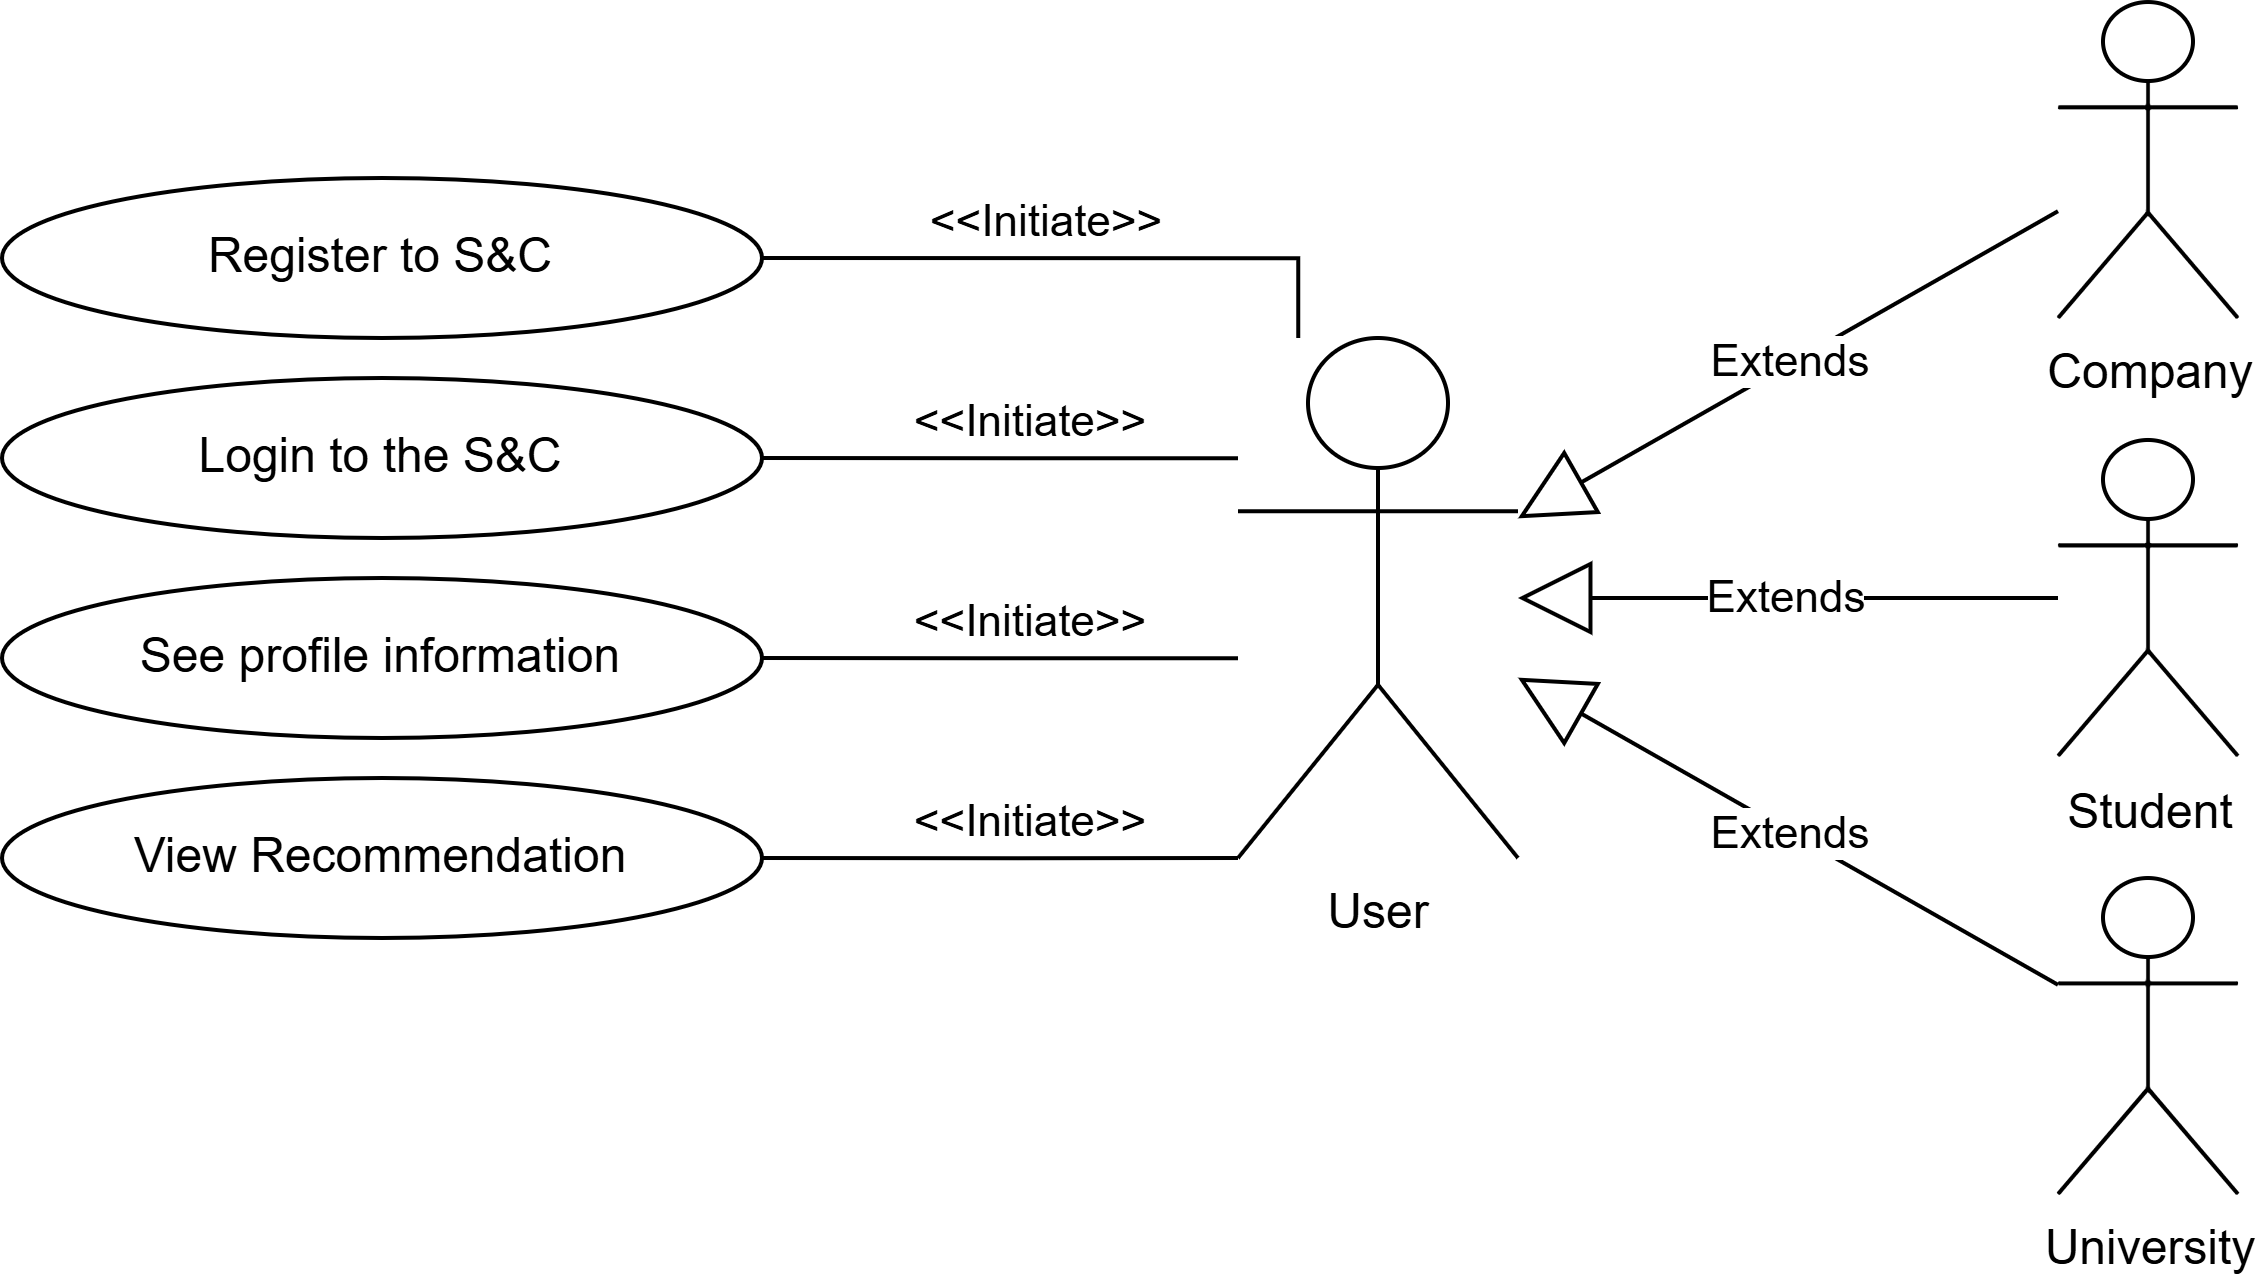
\includegraphics[width=0.8\textwidth]{Images/Use_Case_Diagrams/User_diagram.png}
    \caption{User's Use Case Diagram}
\end{figure}
\begin{figure}[H]
    \centering
    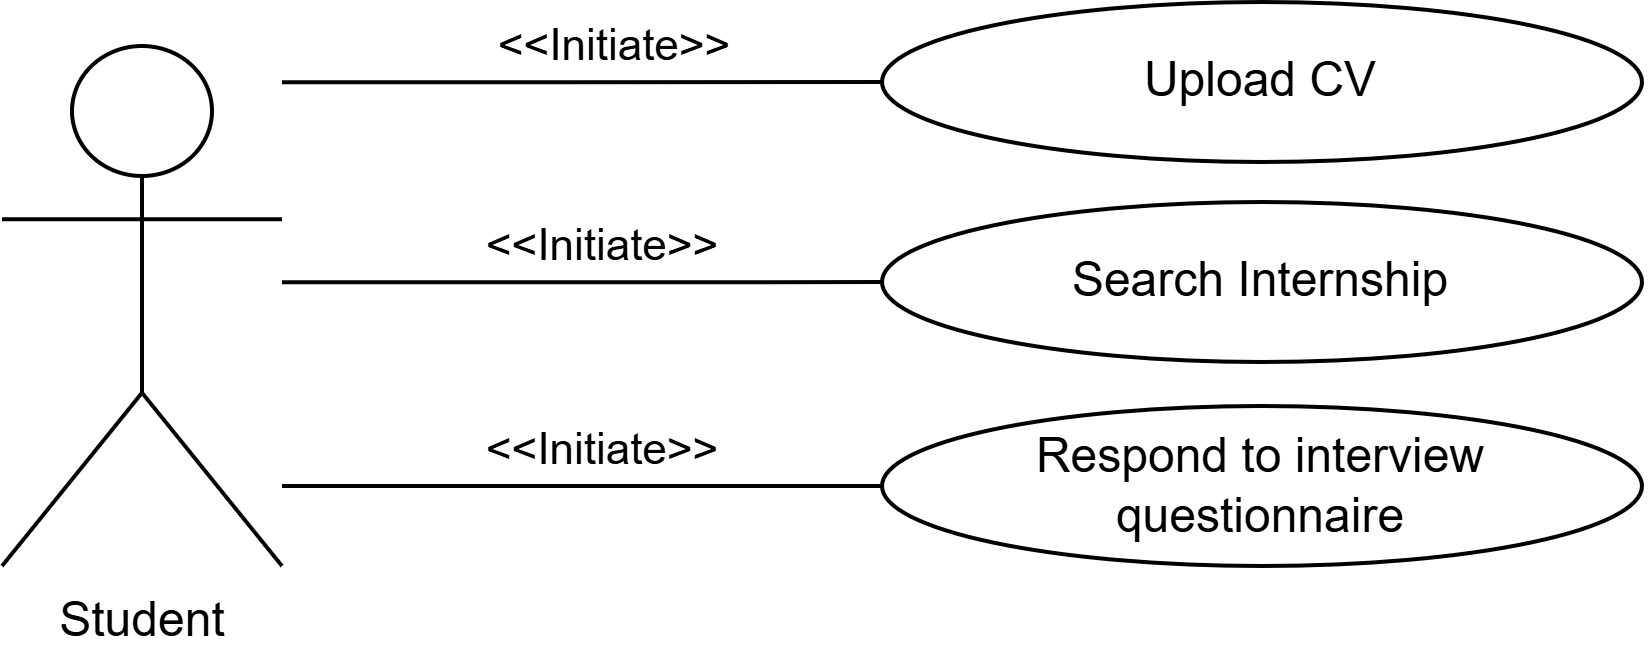
\includegraphics[width=0.7\textwidth]{Images/Use_Case_Diagrams/Student_diagram.png}
    \caption{Student's Use Case Diagram}
\end{figure}
\begin{figure}[H]
    \centering
    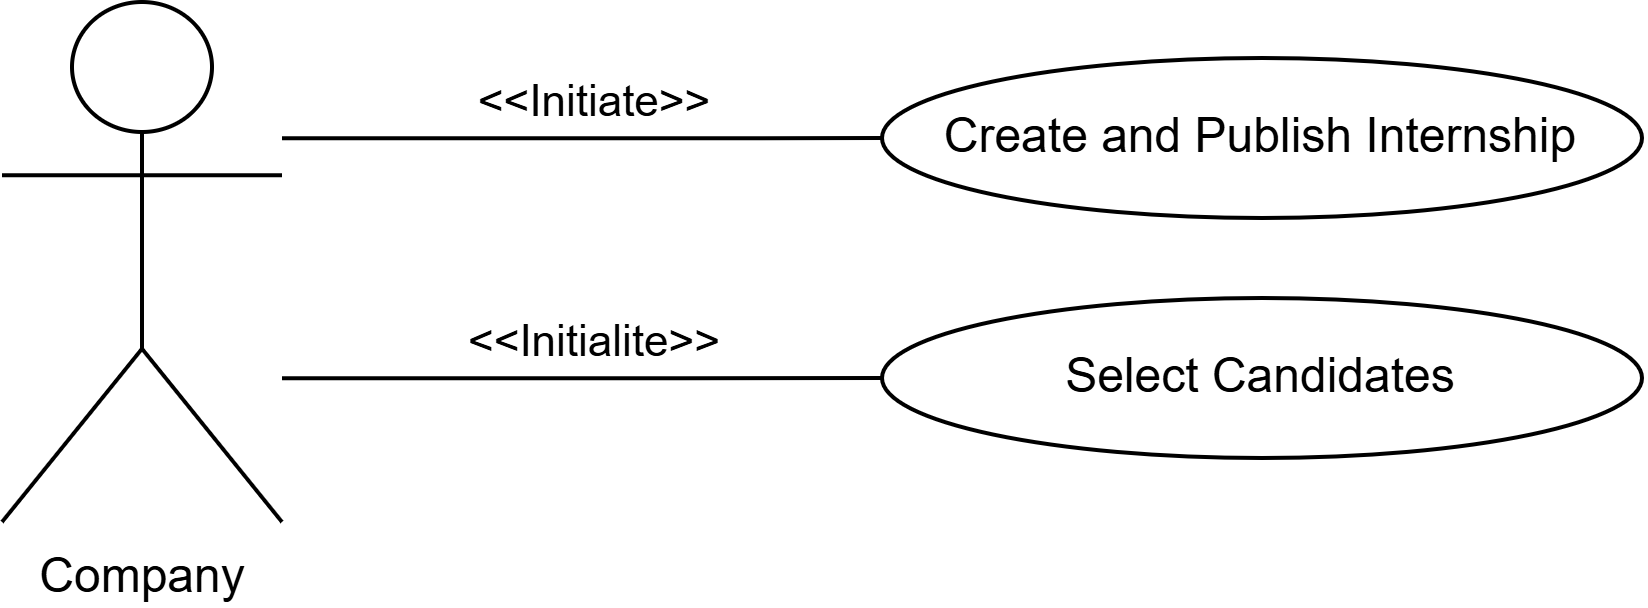
\includegraphics[width=0.7\textwidth]{Images/Use_Case_Diagrams/Company_diagram.png}
    \caption{Company's Use Case Diagram}
\end{figure}
\begin{figure}[H]
    \centering
    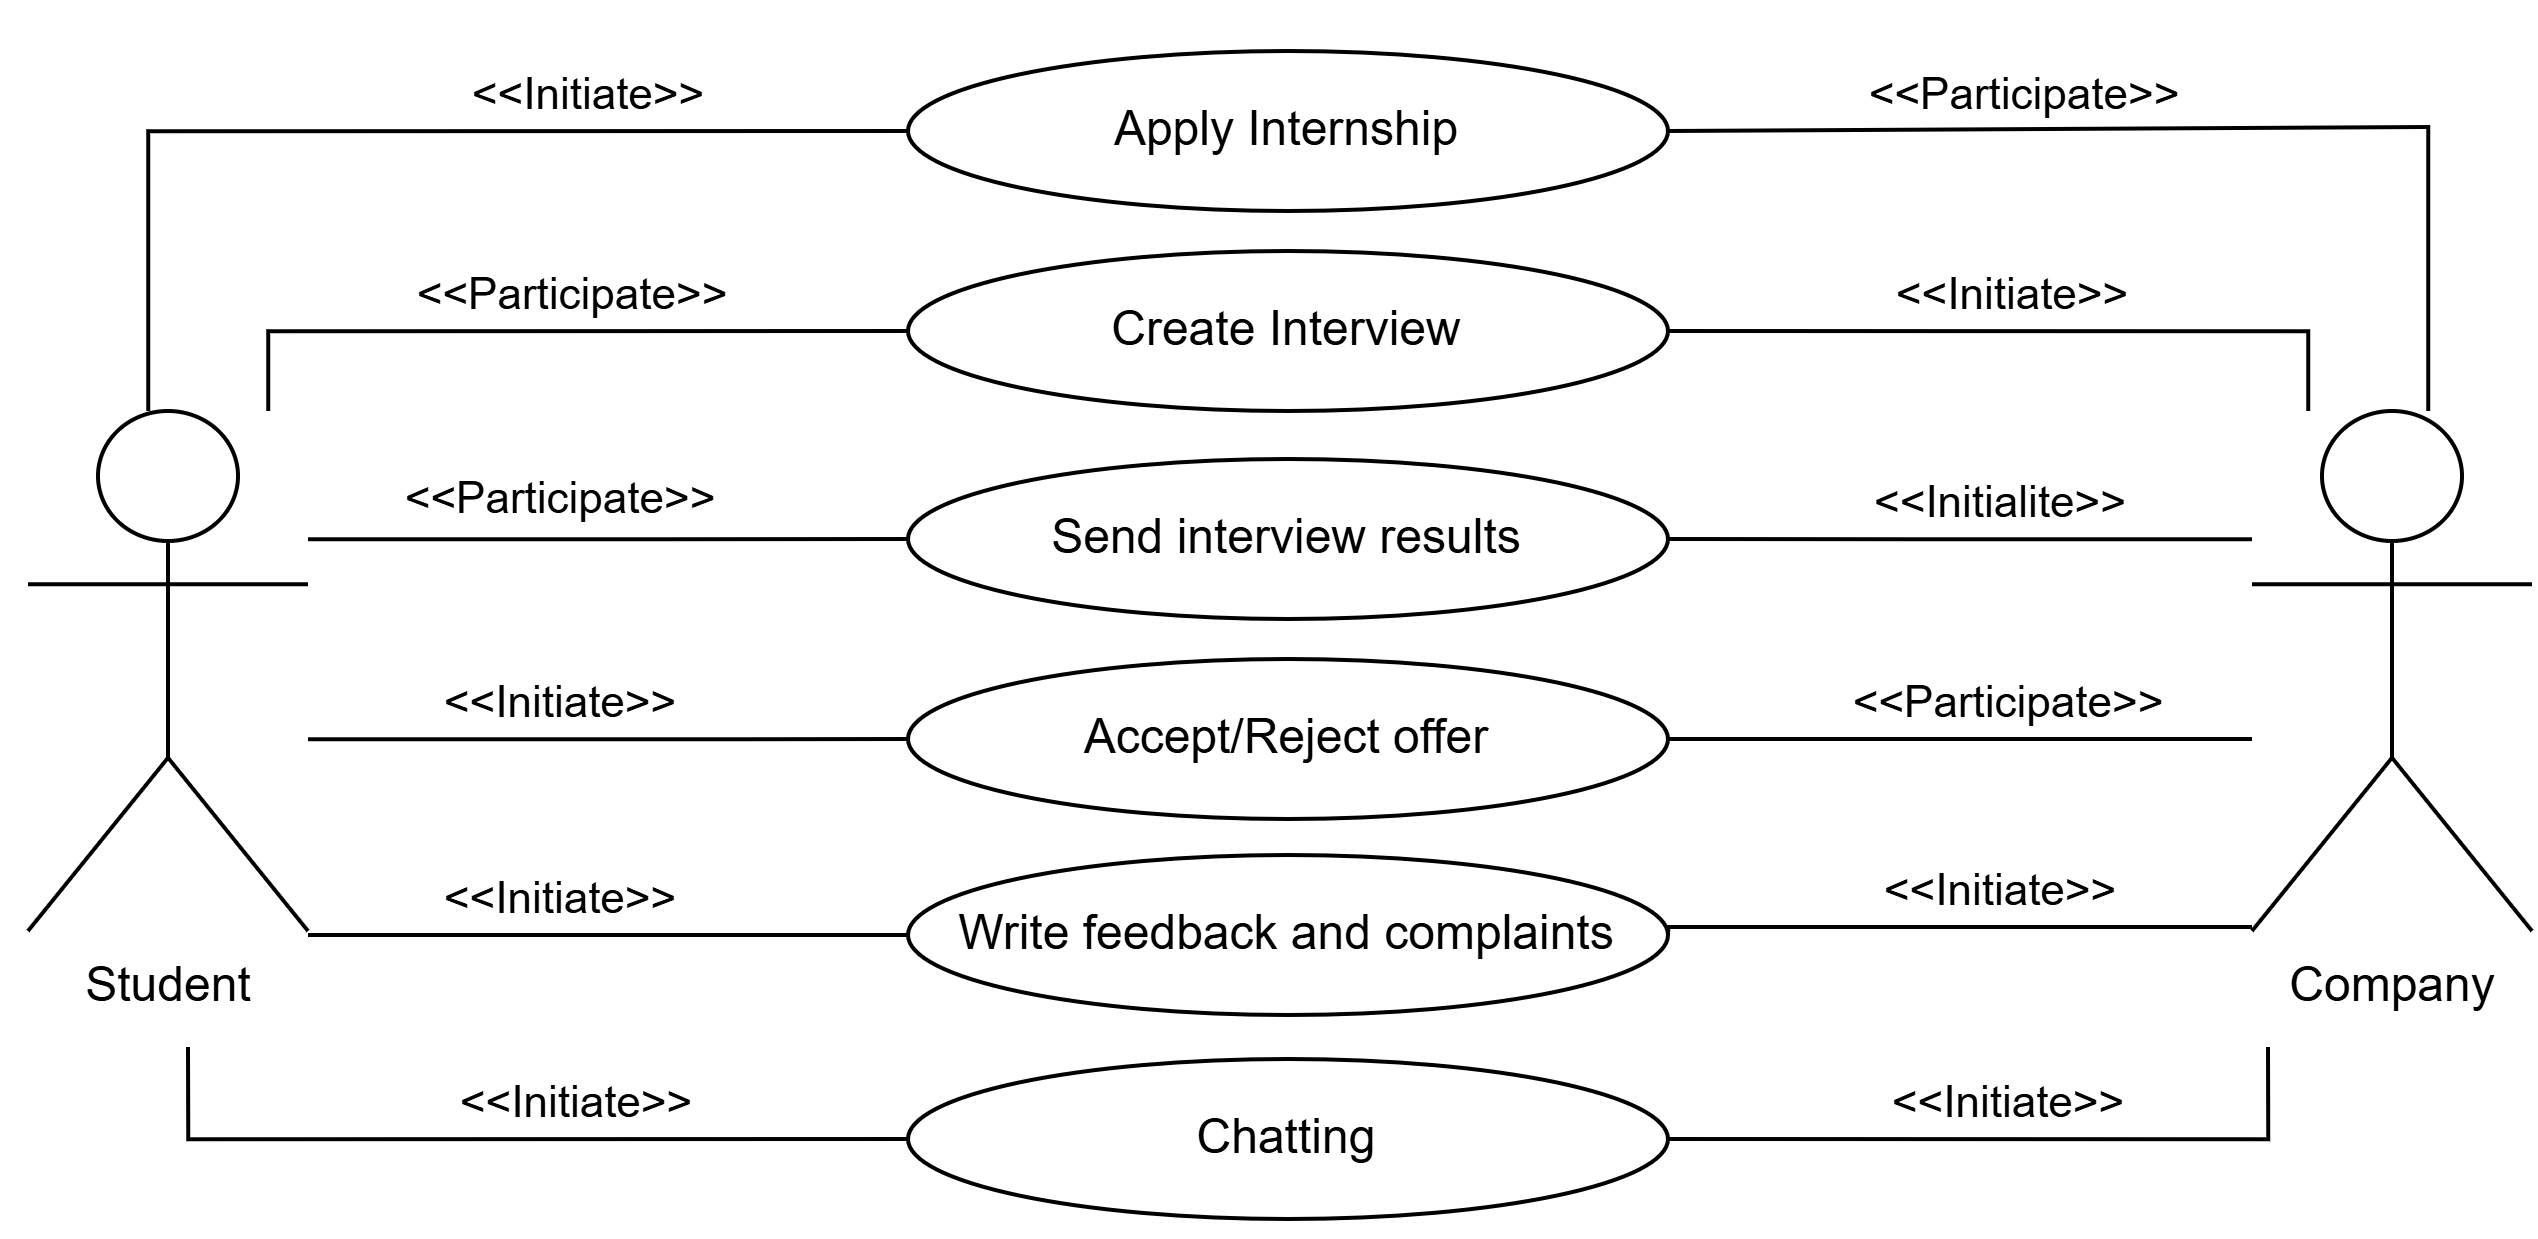
\includegraphics[width=0.9\textwidth]{Images/Use_Case_Diagrams/SandC_diagram.png}
    \caption{Student and Company Use Case Diagram}
\end{figure}
\begin{figure}[H]
    \centering
    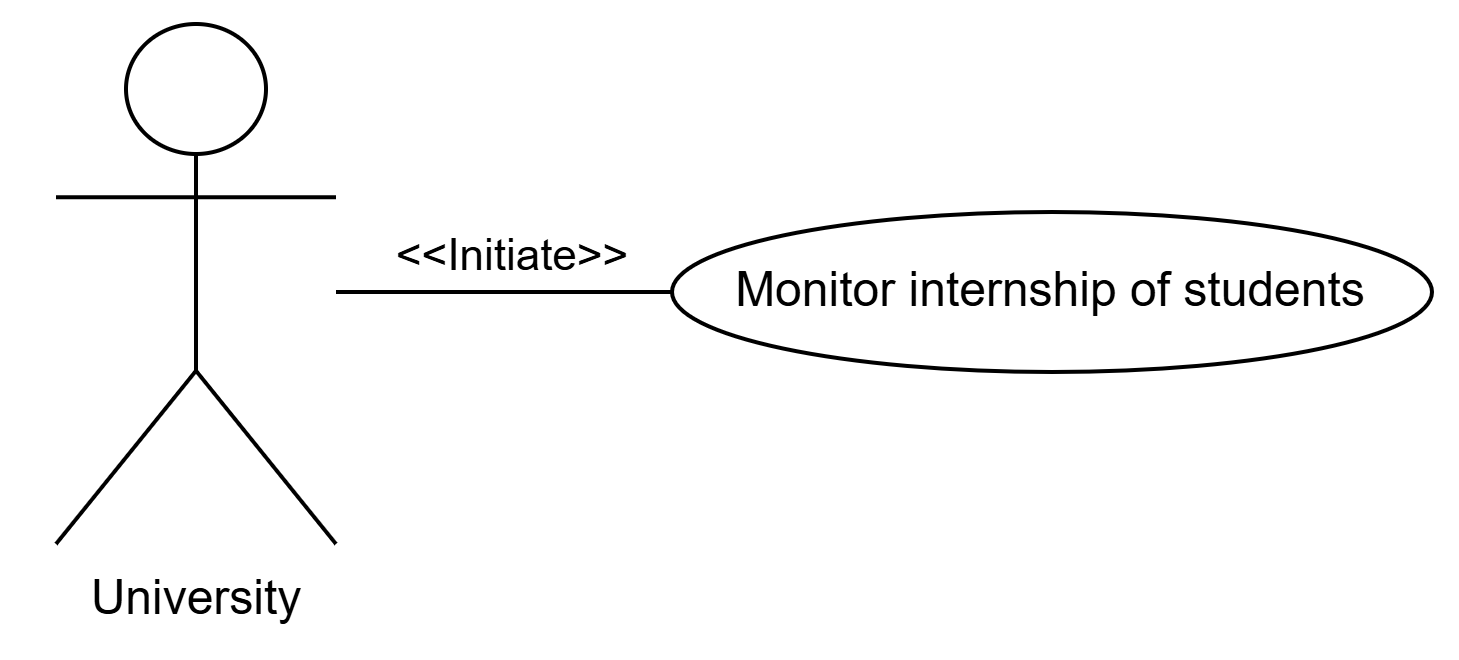
\includegraphics[width=0.6\textwidth]{Images/Use_Case_Diagrams/University_diagram.png}
    \caption{University's Use Case Diagram}
\end{figure}


\subsubsection{Use Case Description}
%Use Case 1
\begin{center}
    \begin{tabular}{|p{9em}|p{27em}|}
        \hline
        \rowcolor{bluepoli!40}
        \textbf{Name} & \textbf{[U1]Register to S\&C} \\
        \hline
        \textbf{Actors} & Unregistered User \\
        \hline
        \textbf{Entry Condition} & 
            \begin{itemize}
                \item A user who does not have an account opens the platform. 
            \end{itemize} \\
        \hline
        \textbf{Events Flow} & 
        \begin{enumerate}
            \item S\&C shows the welcome page.
            \item The user clicks on the ``Create account'' button. 
            \item S\&C shows the registration page.
            \item The user selects the type of account to create by clicking either on the Student or on the Company button.
            \item S\&C shows the respective registration form.
            \item The user fills in the form with the required information, like: email, password, name, surname, interests, university (for the student).
            \item The user clicks on the ``Create account'' button.
            \item S\&C checks the information provided by the user.
            \item S\&C updates the database in order to store all the provided information.
            \item S\&C sends a confirmation email to the user.
            \item The user clicks on the confirmation link in the email.
        \end{enumerate} \\
        \hline
        \textbf{Exit Condition} & The user is now registered and is granted access to the platform. \\
        \hline
        \textbf{Exceptions} & In case the information provided by the user is not valid (step 8 fails), for instance the email is already linked to 
        an account, the system will show an error message and ask to provide the correct information, effectively returning to step 5. \\
        \hline
    \end{tabular}
\end{center}

%Use Case 2
\begin{center}
    \begin{tabular}{|p{9em}|p{27em}|}
        \hline
        \rowcolor{bluepoli!40}
        \textbf{Name} & \textbf{[U2]Login to S\&C} \\
        \hline
        \textbf{Actors} & User \\
        \hline
        \textbf{Entry Condition} & 
        \begin{itemize}
            \item A user who does have an account opens the platform.
        \end{itemize} \\
        \hline
        \textbf{Events Flow} & 
        \begin{enumerate}
            \item S\&C shows the welcome page.
            \item The user fills in the form with the required information, like: email, password.
            \item The user clicks on the Login button.
            \item S\&C checks the information provided by the user.
            \item S\&C displays the Dashboard page. 
        \end{enumerate} \\
        \hline
        \textbf{Exit Condition} & The user is now logged in the platform. \\
        \hline
        \textbf{Exceptions} & In case the information provided by the user is invalid (step 4 fails), for instance the email isn't linked to
        any account or the password is wrong, an error message that asks to provide the correct information is shown, effectively 
        returning to step 2. \\
        \hline
    \end{tabular}
\end{center}

%Use Case 3
\begin{center}
    \begin{tabular}{|p{9em}|p{27em}|}
        \hline
        \rowcolor{bluepoli!40} % comment this line to remove the color
        \textbf{Name} & \textbf{[U3]See profile information} \\
        \hline
        \textbf{Actors} & User \\
        \hline
        \textbf{Entry Condition} & 
        \begin{itemize}
            \item User is logged in with the corresponding account.
            \item S\&C shows the Dashboard page.
        \end{itemize} \\
        \hline
        \textbf{Events Flow} & 
        \begin{enumerate}
            \item User clicks on the Search tab or on the search bar in the dashboard page. 
            \item User types the name of the user they want to search in the search bar.
            \item User click on the Search button.
            \item S\&C shows all the profiles that match the search.
            \item User clicks on the profile they want to see.
            \item S\&C shows the profile information.
        \end{enumerate} \\
        \hline
        \textbf{Exit Condition} & 
            S\&C displayed the profile information requested by the user.\\
        \hline
        \textbf{Exceptions} &
            If no profile is found, a message will be displayed saying that the profile does not exist.\\
        \hline
    \end{tabular}
\end{center}

%Use Case 4
\begin{center}
    \begin{tabular}{|p{9em}|p{27em}|}
        \hline
        \rowcolor{bluepoli!40} % comment this line to remove the color
        \textbf{Name} & \textbf{[U4]View recommendation} \\
        \hline
        \textbf{Actors} & Student, Company \\
        \hline
        \textbf{Entry Condition} & 
        \begin{itemize}
            \item Student is logged.
            \item Company is logged.
            \item S\&C shows the Dashboard page.
        \end{itemize} \\
        \hline
        \textbf{Events Flow} & 
        \begin{enumerate}
            \item S\&C displays the recommendation section in the Dashboard page.
            \item The student or company browses the recommendations.
            \item The student or company clicks on the recommendation they want to see.
            \item S\&C shows the recommendation details.
            \item The student or company can either accept the recommendation (by applying for the internship, or inviting the 
            student to take part in an internship) or ignore it.
        \end{enumerate} \\
        \hline
        \textbf{Exit Condition} & 
        S\&C displays the recommendation details to the student or company and allows them to do the desired action. \\
        \hline
        \textbf{Exceptions} & 
        If there are not enough data to provide a recommendation related to the student or company, S\&C will show a message
        that no recommendation is available. \\
        \hline
    \end{tabular}
\end{center}

%Use Case 5
\begin{center}
    \begin{tabular}{|p{9em}|p{27em}|}
        \hline
        \rowcolor{bluepoli!40} % comment this line to remove the color
        \textbf{Name} & \textbf{[U5]Upload CV} \\
        \hline
        \textbf{Actors} & Student \\
        \hline
        \textbf{Entry Condition} & 
        \begin{itemize}
            \item Student is logged.
            \item Student opens the profile modification page.
            \item Student has a CV file to upload.
        \end{itemize} \\
        \hline
        \textbf{Events Flow} & 
        \begin{enumerate}
            \item The student clicks on the Edit profile button.
            \item S\&C shows the profile modification page.
            \item The student clicks on the Upload CV button.
            \item S\&C shows the file explorer.
            \item The student selects the CV file and uploads it.
            \item S\&C checks the file format and size.
            \item The students clicks on the Save button.
            \item S\&C stores the file in the database.
            \item S\&C displays the updated profile page.
        \end{enumerate} \\
        \hline
        \textbf{Exit Condition} & The student's CV is uploaded and displayed in the profile page. \\
        \hline
        \textbf{Exceptions} & In case the file format or size is not valid (step 6 fails), the system will show an error message and ask 
        to upload only files in \.pdf format, effectively returning to step 2. \\
        \hline
    \end{tabular}
\end{center}

%Use Case 6
\begin{center}
    \begin{tabular}{|p{9em}|p{27em}|}
        \hline
        \rowcolor{bluepoli!40} % comment this line to remove the color
        \textbf{Name} & \textbf{[U6]Search internship} \\
        \hline
        \textbf{Actors} & Student \\
        \hline
        \textbf{Entry Condition} &  
        \begin{itemize}
            \item Student is logged.
            \item S\&C shows the Dashboard page.
            \item The student wants to search for an internship.
        \end{itemize} \\
        \hline
        \textbf{Events Flow} & 
        \begin{enumerate}
            \item The student clicks on the Search tab or on the search bar in the Dashboard page.
            \item The student types the keyword in the search bar.
            \item The student clicks on the Search button.
            \item S\&C shows the internships that match the keyword.
            \item The student either clicks on an internship to see more details or scrolls down to see more internships.
        \end{enumerate} \\
        \hline
        \textbf{Exit Condition} & The student has found the internship they were looking for. The student does not find what they were looking for,
        so they close the search page or retry a new search. \\
        \hline
        \textbf{Exceptions} & In case the keyword doesn't match any internship (step 4 fails), S\&C shows the message: "No internship was found,
        please try with a different keyword", effectively returning to step 2. \\
        \hline
    \end{tabular}
\end{center}

%Use Case 7
\begin{center}
    \begin{tabular}{|p{9em}|p{27em}|}
        \hline
        \rowcolor{bluepoli!40}
        \textbf{Name} & \textbf{[U7]Apply internship} \\
        \hline
        \textbf{Actors} & Student \\
        \hline
        \textbf{Entry Condition} & 
        \begin{itemize}
            \item Student is logged.
            \item S\&C shows the Internship details page.
            \item The student wants to apply to the internship.
        \end{itemize} \\
        \hline
        \textbf{Events Flow} & 
        \begin{enumerate}
            \item The student clicks on the Apply button.
            \item S\&C gets the student's information from the database.
            \item S\&C checks that the student has not already applied for that internship or is starting an internship in the same period.
            \item S\&C creates and stores the application in the database.
            \item S\&C shows the details of the application in the My applications page.
        \end{enumerate} \\
        \hline
        \textbf{Exit Condition} & The student has applied for the internship. \\
        \hline
        \textbf{Exceptions} & The student has already applied for that internship (step 3 fails), S\&C will show an error message and ask to
        check the My applications page to see the status of the application. 
        
        The student has already accepted an offer for another internship which start in the same period (step 3 fails), S\&C will show an 
        error message and ask to check the My Internship page to see the current internship.\\
        \hline
    \end{tabular}
\end{center}

%Use Case 8
\begin{center}
    \begin{tabular}{|p{9em}|p{27em}|}
        \hline
        \rowcolor{bluepoli!40} % comment this line to remove the color
        \textbf{Name} & \textbf{[U8]Create interview} \\
        \hline
        \textbf{Actors} & Company, Student \\
        \hline
        \textbf{Entry Condition} & 
        \begin{itemize}
            \item Company is logged in with the corresponding account.
            \item Company has a list of students selected to create the interview for.
            \item Student is selected by the company for the interview process.
        \end{itemize} \\
        \hline
        \textbf{Events Flow} & 
        \begin{enumerate}
            \item Company sets up the questions that will be asked to the student in the questionnaire and other information about the interview.
            \item Company clicks on the ``Submit'' button.
            \item S\&C checks the list of students and the information filled by the company.
            \item S\&C stores the data in the database.
            \item S\&C sends a notification to Student about the interview.
        \end{enumerate} \\
        \hline
        \textbf{Exit Condition} & 
        Information related to the interview is received and stored by S\&C, the interview information is updated and the notification is 
        sent to the student who is waiting for the interview process to start.\\
        \hline
        \textbf{Exceptions} &
        The student selected by the company has already been accepted by another company and has started the internship at the same time.
        Then the system will notify the company that to select another student from the list of the candidates.\\
        \hline
    \end{tabular}
\end{center}

%Use Case 9
\begin{center}
    \begin{tabular}{|p{9em}|p{27em}|}
        \hline
        \rowcolor{bluepoli!40} % comment this line to remove the color
        \textbf{Name} & \textbf{[U9]Respond to interview questionnaire} \\
        \hline
        \textbf{Actors} & Student\\
        \hline
        \textbf{Entry Condition} & 
        \begin{itemize}
            \item Student is logged.
            \item Student was selected by the company for the interview process.
        \end{itemize} \\
        \hline
        \textbf{Events Flow} & 
        \begin{enumerate}
            \item Student clicks on the notification informing them about the interview or opens the interview page from the application page.
            \item S\&C shows the interview questionnaire.
            \item Student fills in the questionnaire.
            \item Student clicks on the ``Submit'' button.
            \item S\&C checks the answers provided by the student.
            \item S\&C stores the student's answers in the database.
            \item S\&C updates the status of the student's application.
        \end{enumerate} \\
        \hline
        \textbf{Exit Condition} & S\&C shows the student that the questionnaire has been submitted successfully.\\
        \hline
        \textbf{Exceptions} & The student does not correctly fill in the questionnaire (step 5 fails), S\&C will ask the student to correctly
        fill the questionnaire, effectively returning to step 2.\\
        \hline
    \end{tabular}
\end{center}

%Use Case 10
\begin{center}
    \begin{tabular}{|p{9em}|p{27em}|}
        \hline
        \rowcolor{bluepoli!40} % comment this line to remove the color
        \textbf{Name} & \textbf{[U10]Send interview results} \\
        \hline
        \textbf{Actors} & Company, Student\\
        \hline
        \textbf{Entry Condition} & 
        \begin{itemize}
            \item Student is logged.
            \item Company is logged.
            \item Company has to decide who to accept for the internship.
        \end{itemize} \\
        \hline
        \textbf{Events Flow} & 
        \begin{enumerate}
            \item The Company opens the Internship Management page.
            \item The Company clicks on Interview Management page.
            \item S\&C shows the list of students who have completed the questionnaire.
            \item The Company selects the students to accept for the internship.
            \item The Company clicks on the Send results button.
            \item S\&C checks the list of students selected by the company.
            \item S\&C stores the data in the database.
            \item S\&C sends a notification to the students who have been accepted, asking them to confirm or reject the offer.
        \end{enumerate} \\
        \hline
        \textbf{Exit Condition} & The company has sent the results of the interview to the students.\\
        \hline
        \textbf{Exceptions} & There is a problem with the company selection (step 6 fails), S\&C will notify the company that the selection
        has not been saved and ask to try again, effectively returning to step 3.\\
        \hline
    \end{tabular}
\end{center}

%Use Case 11
\begin{center}
    \begin{tabular}{|p{9em}|p{27em}|}
        \hline
        \rowcolor{bluepoli!40} % comment this line to remove the color
        \textbf{Name} & \textbf{[U11]Accept/reject offer} \\
        \hline
        \textbf{Actors} & Company, Student\\
        \hline
        \textbf{Entry Condition} & 
        \begin{itemize}
            \item Student is logged in with the corresponding account.
            \item Student has received an offer from the company.
            \item Company is waiting for the student response.
        \end{itemize} \\
        \hline
        \textbf{Events Flow} & 
        \begin{enumerate}
            \item Student click on the notification regarding the offer.
            \item S\&C displays the details to the student and asks to accept or reject the offer.
            \item Student clicks on the ``accept'' or ``reject'' button.
            \item S\&C checks the student's choice and sends a notification to the related company.
            \item S\&C registers the student's decision and updates the status of the student's application.
        \end{enumerate} \\
        \hline
        \textbf{Exit Condition} & 
         The student's decision is saved in the system, the status of the application of the student is updated, and the company
         who has sent the offer is notified about the student's decision.\\
        \hline
        \textbf{Exceptions} &
        The student has already accepted another internship. S\&C will notify the student that they cannot accept more than one offer if 
        the two internships start in the same period.

        The deadline for accepting the offer has passed. The system will notify the student that it is too late to accept the offer.\\
        \hline
    \end{tabular}
\end{center}

%Use Case 12
\begin{center}
    \begin{tabular}{|p{9em}|p{27em}|}
        \hline
        \rowcolor{bluepoli!40} % comment this line to remove the color
        \textbf{Name} & \textbf{[U12]Write feedback and complaints} \\
        \hline
        \textbf{Actors} & Company, Student\\
        \hline
        \textbf{Entry Condition} & 
        \begin{itemize}
            \item Student and Company are logged in.
            \item Student and company have taken part in an active internship.
        \end{itemize} \\
        \hline
        \textbf{Events Flow} & 
        \begin{enumerate}
            \item Student or company clicks on the active internship which they want to leave comments on.
            \item S\&C displays the feedback and complaints page related to that internship.
            \item Student or company writes in the box dedicated to the comments.
            \item Student or company clicks on the ``Submit'' button.
            \item S\&C stores the comments and displays them on the evaluation page.
            \item S\&C notifies the Student and company that there is a new feedback or complaint regarding specific internship.
        \end{enumerate} \\
        \hline
        \textbf{Exit Condition} & 
         The comments are stored in the database and displayed on the internship evaluation page. 
         The student and company are notified about the new feedback.\\
        \hline
        \textbf{Exceptions} &
        The student or company send an empty comment, the system will notify them that the comment can not be empty.\\
        \hline
    \end{tabular}
\end{center}

%Use Case 13
\begin{center}
    \begin{tabular}{|p{9em}|p{27em}|}
        \hline
        \rowcolor{bluepoli!40} % comment this line to remove the color
        \textbf{Name} & \textbf{[U13]Chatting} \\
        \hline
        \textbf{Actors} & Company, Student\\
        \hline
        \textbf{Entry Condition} & 
        \begin{itemize}
            \item Student and Company are logged in.
        \end{itemize} \\
        \hline
        \textbf{Events Flow} & 
        \begin{enumerate}
            \item Student or company clicks on the chat icon.
            \item S\&C displays the list of the available chats.
            \item Student or company selects the chat where they want write.
            \item Student or company write the message in the message box and click on the ``Send'' button.
            \item S\&C receives the message and stores it in the chat history database.
            \item S\&C sends it to the recipient and displays it in the chat.
            \item S\&C notifies the recipient that there is a new message.
        \end{enumerate} \\
        \hline
        \textbf{Exit Condition} & 
         The message is correctly sent and stored by S\&C. The recipient and the sender's chat history are updated and the recipient is
         notified about the new message incoming, the message details are displayed successfully in the chat.\\
        \hline
        \textbf{Exceptions} &
         If the content of the message is empty, S\&C will notify the sender that the message can not be empty.

         If there is no chat available in the chat list, S\&C will display a message saying the chats will be available when the student or 
         company will have taken part in an internship at least once.\\
        \hline
    \end{tabular}
\end{center}

%Use Case 14
\begin{center}
    \begin{tabular}{|p{9em}|p{27em}|}
        \hline
        \rowcolor{bluepoli!40} % comment this line to remove the color
        \textbf{Name} & \textbf{[U14]Create and Publish Internship} \\
        \hline
        \textbf{Actors} & Company \\
        \hline
        \textbf{Entry Condition} & 
        \begin{itemize}
            \item Company is logged in with the corresponding account.
            \item Company has all necessary information to create an internship announcement.
        \end{itemize} \\
        \hline
        \textbf{Events Flow} & 
        \begin{enumerate}
            \item Company opens the ``Publish internship'' page.
            \item S\&C displays the page with the form to fill in the internship announcement details.
            \item Company inserts the data needed to complete the form and clicks on the ``Submit'' button.
            \item S\&C checksthe data inserted by the company and stores it in the database.
            \item S\&C displays updated list of the internship available related to this company.
            \item S\&C displays the internship announcement on the platform.
        \end{enumerate} \\
        \hline
        \textbf{Exit Condition} & 
        S\&C successfully displays the internship announcement on the platform.\\
        \hline
        \textbf{Exceptions} &
        If there is a missing field in the form, S\&C will notify the company that all fields are required to be filled.

        If the company has already published the announcement with the same content and it is still active, S\&C will notify the company
        that the announcement already exist.\\
        \hline
    \end{tabular}
\end{center}

%Use Case 15
\begin{center}
    \begin{tabular}{|p{9em}|p{27em}|}
        \hline
        \rowcolor{bluepoli!40} % comment this line to remove the color
        \textbf{Name} & \textbf{[U15]Select Candidates} \\
        \hline
        \textbf{Actors} & Company, Student\\
        \hline
        \textbf{Entry Condition} & 
        \begin{itemize}
            \item Student and Company are logged in.
            \item Company has published an internship and the application deadline has passed.
            \item Student has applied for this internship.
        \end{itemize} \\
        \hline
        \textbf{Events Flow} & 
        \begin{enumerate}
            \item Company clicks on the internship announcement which they wants to select the candidates.
            \item S\&C displays the Internship management page.
            \item Company clicks on the ``Select candidates'' button.
            \item S\&C displays the list of the students who have submitted the application.
            \item Company clicks on the student's profile to see the details, in particular the CV.
            \item S\&C displays the student's profile and CV to the company.
            \item Company selects the students who will be invited for the interview.
            \item Company click on the ``Submit'' button.
            \item S\&C stores the list of the selected students and notifies them about the application result in this phase.
            \item S\&C updates the status of the applications of the students who have applied for this internship.
        \end{enumerate} \\
        \hline
        \textbf{Exit Condition} & 
        S\&C stores the decision of the company and updates the status of the application of the students and notifies them about the result.\\
        \hline
        \textbf{Exceptions} &
         If the company has selected a student who has already accepted an offer from another company, S\&C will notify the company 
         that the student has already accepted an offer from another company, and ask to select another student from the list of the candidates.

         If the number of selected students is less or more than the number of the students specified in announcement, S\&C will notify the company to 
         select more or fewer students.\\
        \hline
    \end{tabular}
\end{center}

%Use Case 16
\begin{center}
    \begin{tabular}{|p{9em}|p{27em}|}
        \hline
        \rowcolor{bluepoli!40} % comment this line to remove the color
        \textbf{Name} & \textbf{[U16]Monitor internship of students} \\
        \hline
        \textbf{Actors} & University \\
        \hline
        \textbf{Entry Condition} & 
        \begin{itemize}
            \item A university is logged in with the corresponding account.
            \item The university has students who have taken part in internships.
            \item The university representative wants to monitor the internship process of the students.
        \end{itemize} \\
        \hline
        \textbf{Events Flow} & 
        \begin{enumerate}
            \item S\&C shows the Dashboard page with the list of all registered students of the university.
            \item The University representative clicks on a student's profile.
            \item S\&C shows the student's profile page.
            \item The University representative clicks on one of the student's internships (current or past).
            \item S\&C shows the internship details page.
            \item The University representative can see the feedback and complaints from both parties involved related to that internship.
        \end{enumerate} \\
        \hline
        \textbf{Exit Condition} & The university representative has monitored all the internship processes of the students that they were
        interested in. \\
        \hline
        \textbf{Exceptions} & If the student has not taken part in any internship, S\&C will communicate this to the representative with a 
        message that says "This student has not taken part in any internship yet". \\
        \hline
    \end{tabular}
\end{center}


\subsubsection{Sequence Diagrams}
% Use Case 1
\begin{figure}[H]
    \centering
    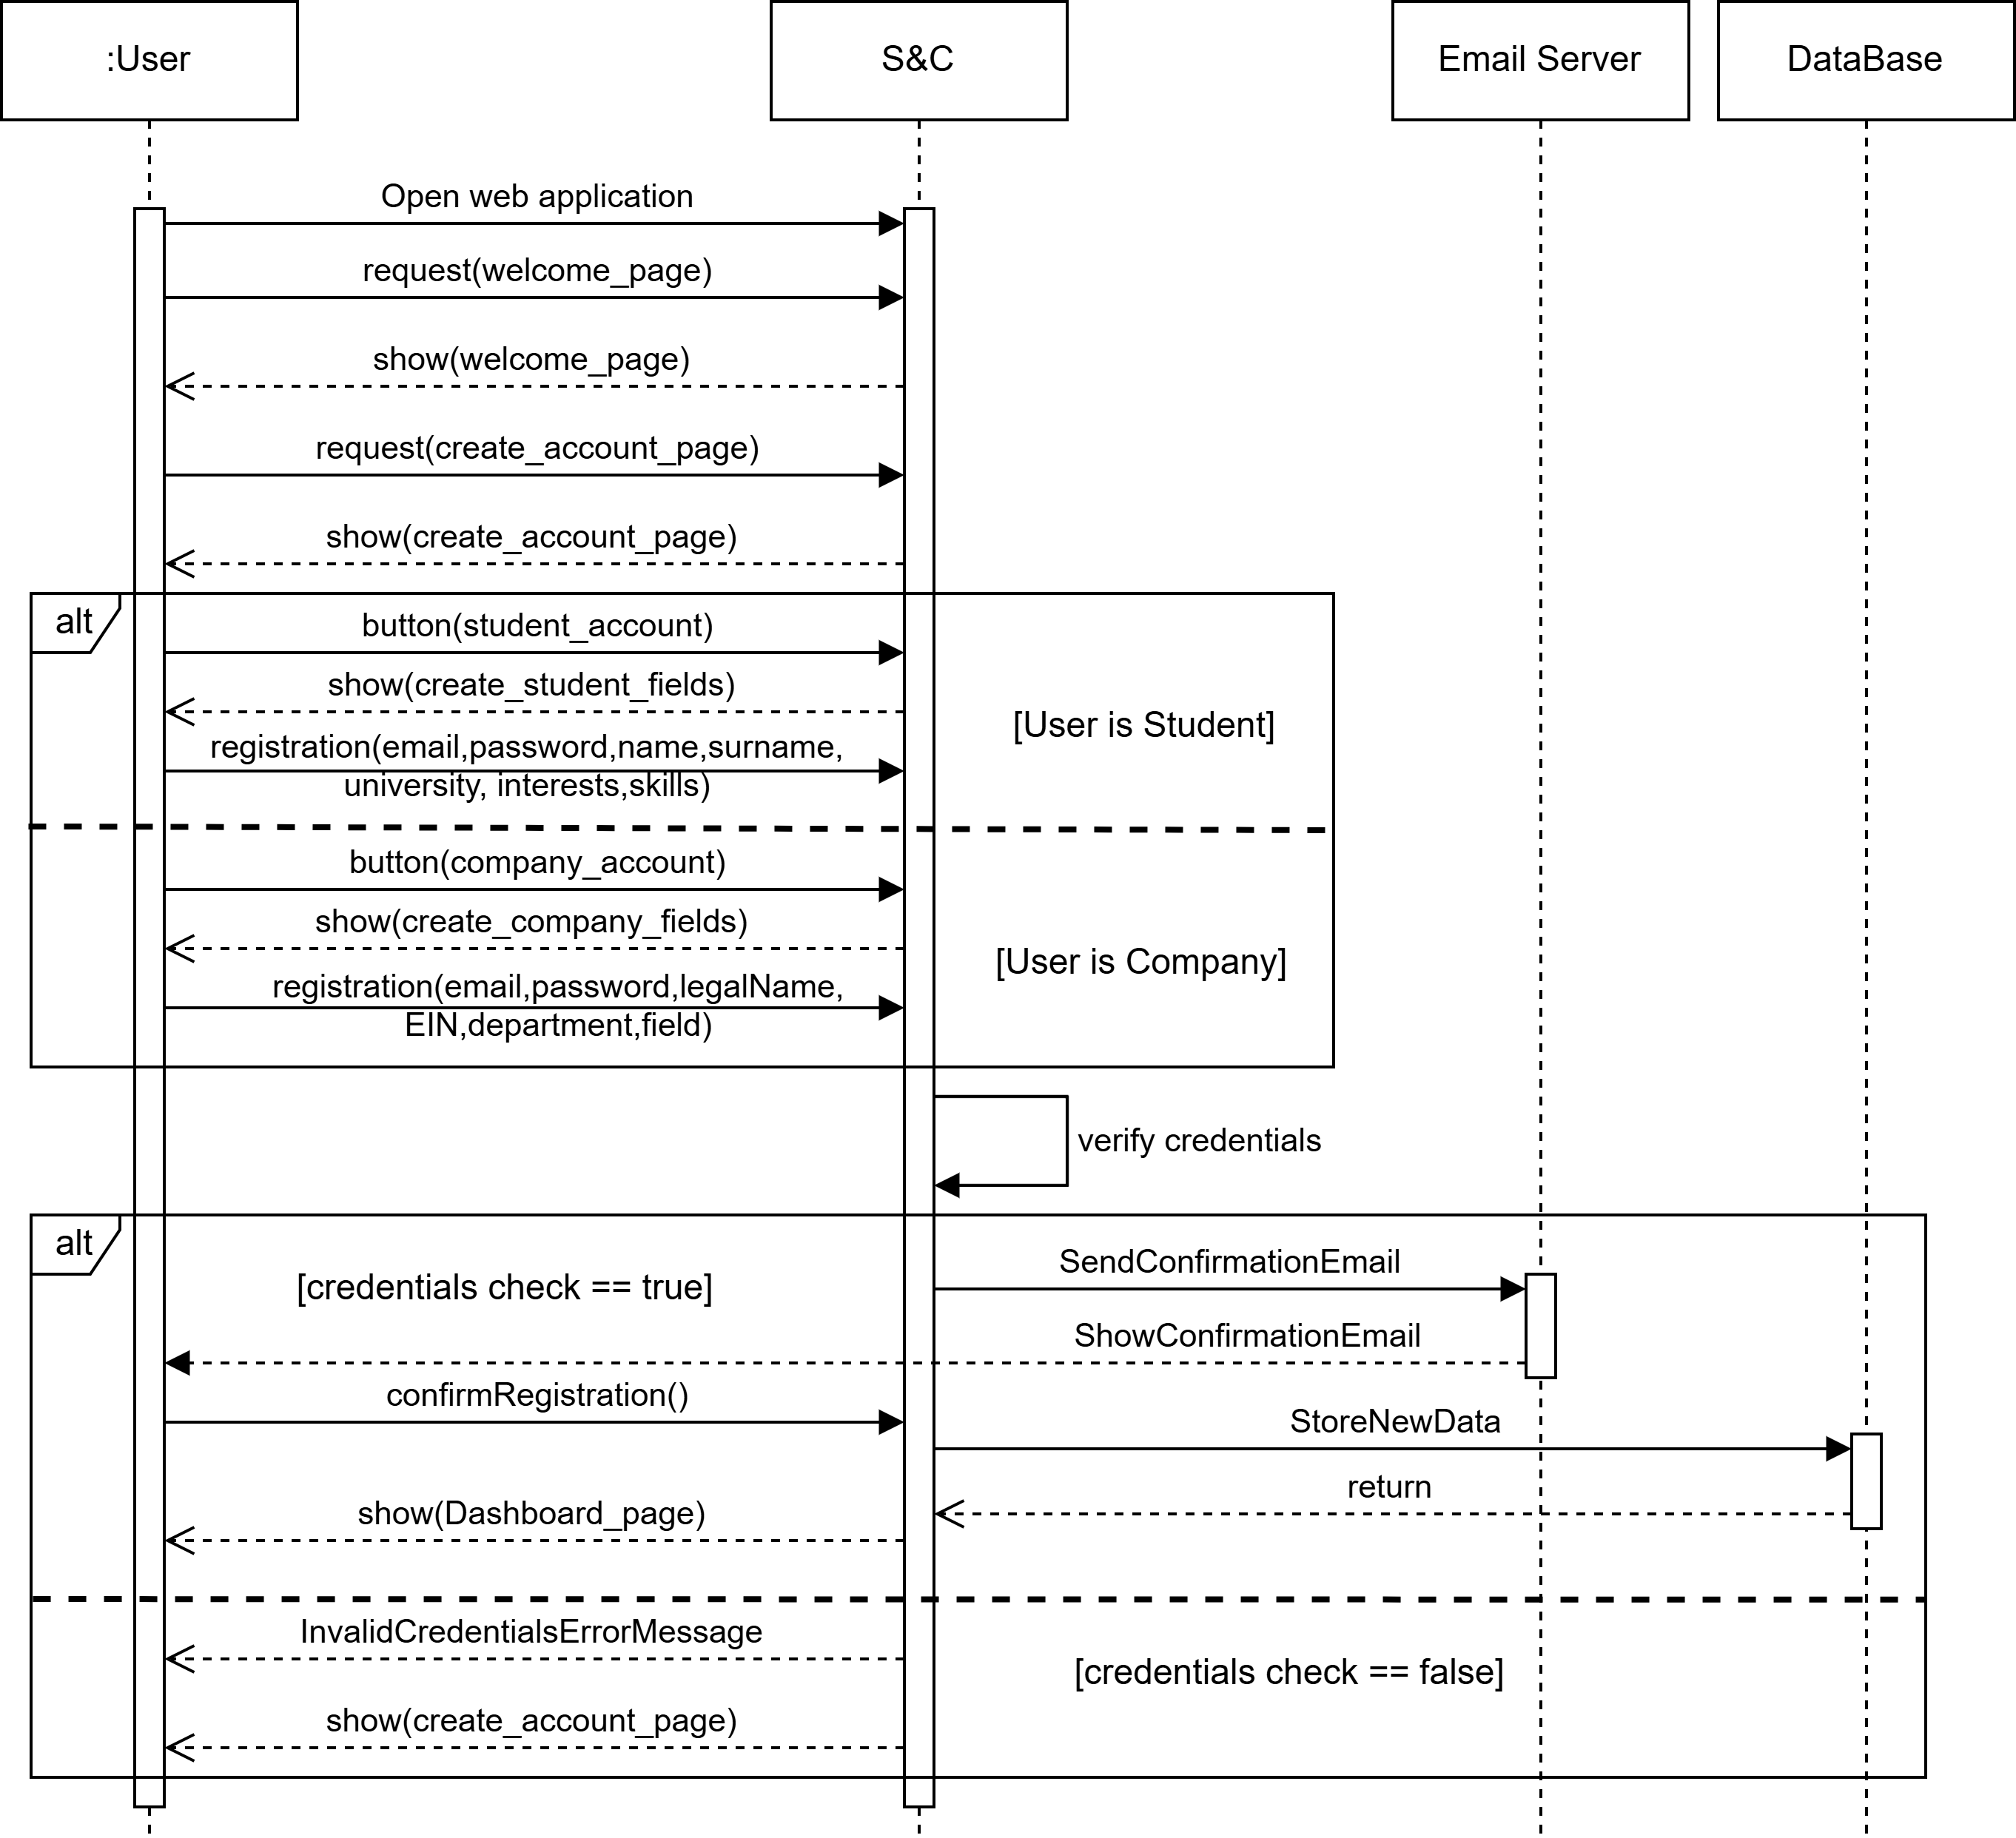
\includegraphics[width=1\textwidth]{Images/Sequence_Diagrams/registration_SD.png}
    \caption{Registration to S\&C Sequence Diagram}
\end{figure}
% Use Case 2
\begin{figure}[H]
    \centering
    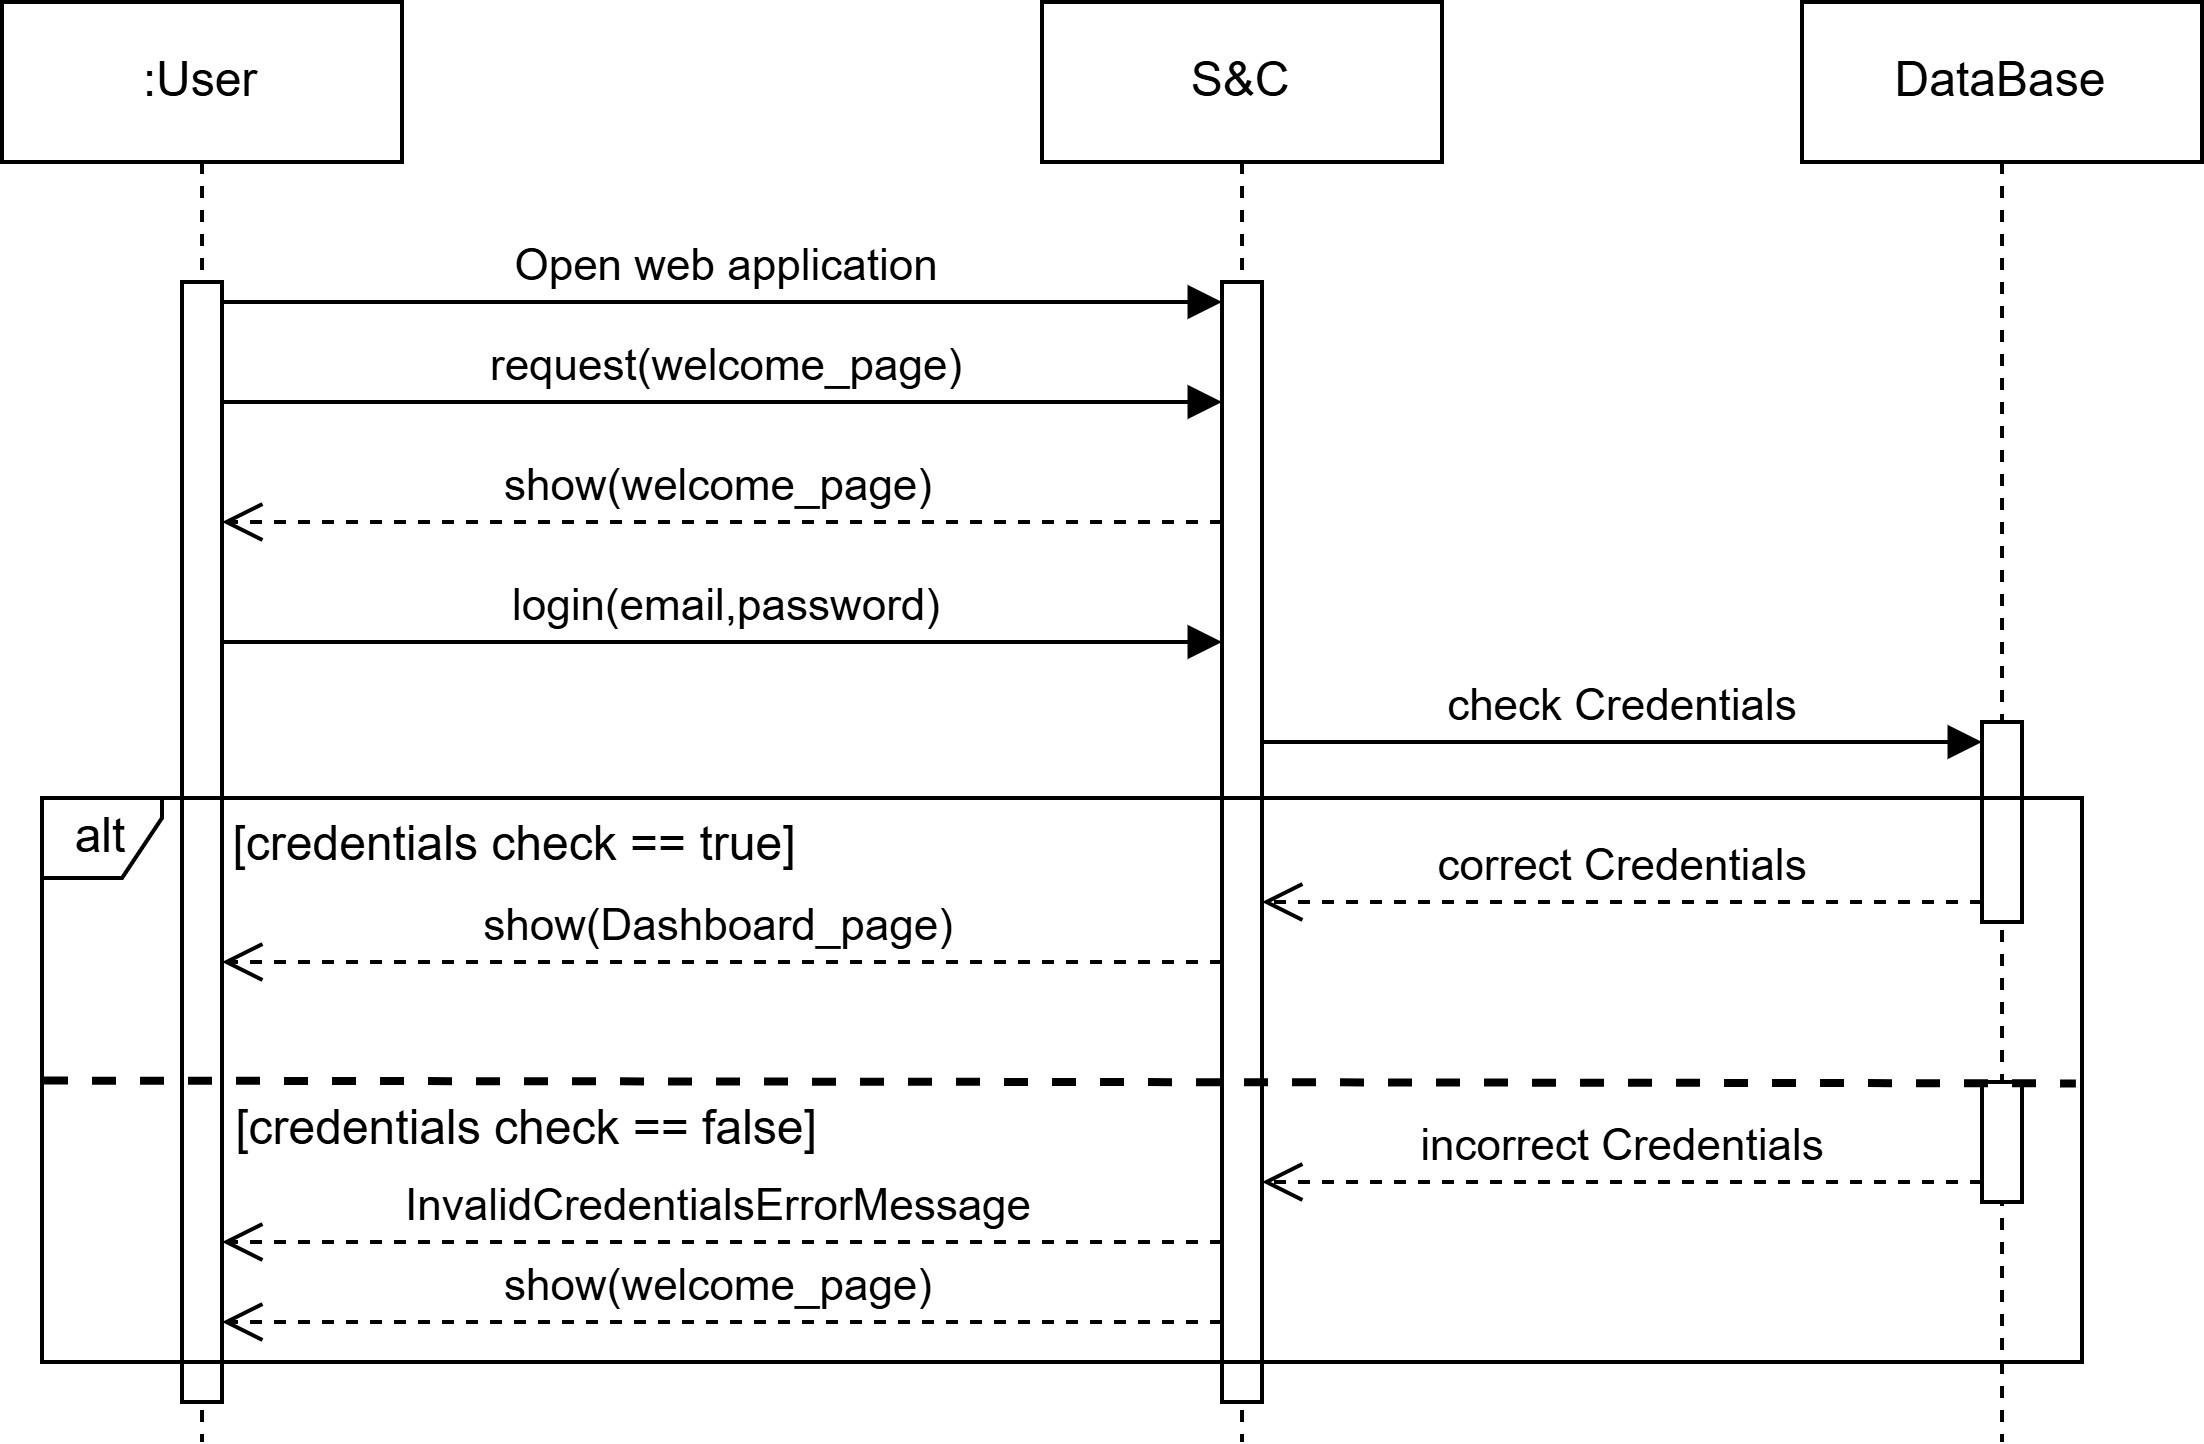
\includegraphics[width=0.75\textwidth]{Images/Sequence_Diagrams/login_SD.png}
    \caption{Login to S\&C Sequence Diagram}
\end{figure}
% Use Case 3
\begin{figure}[H]
    \centering
    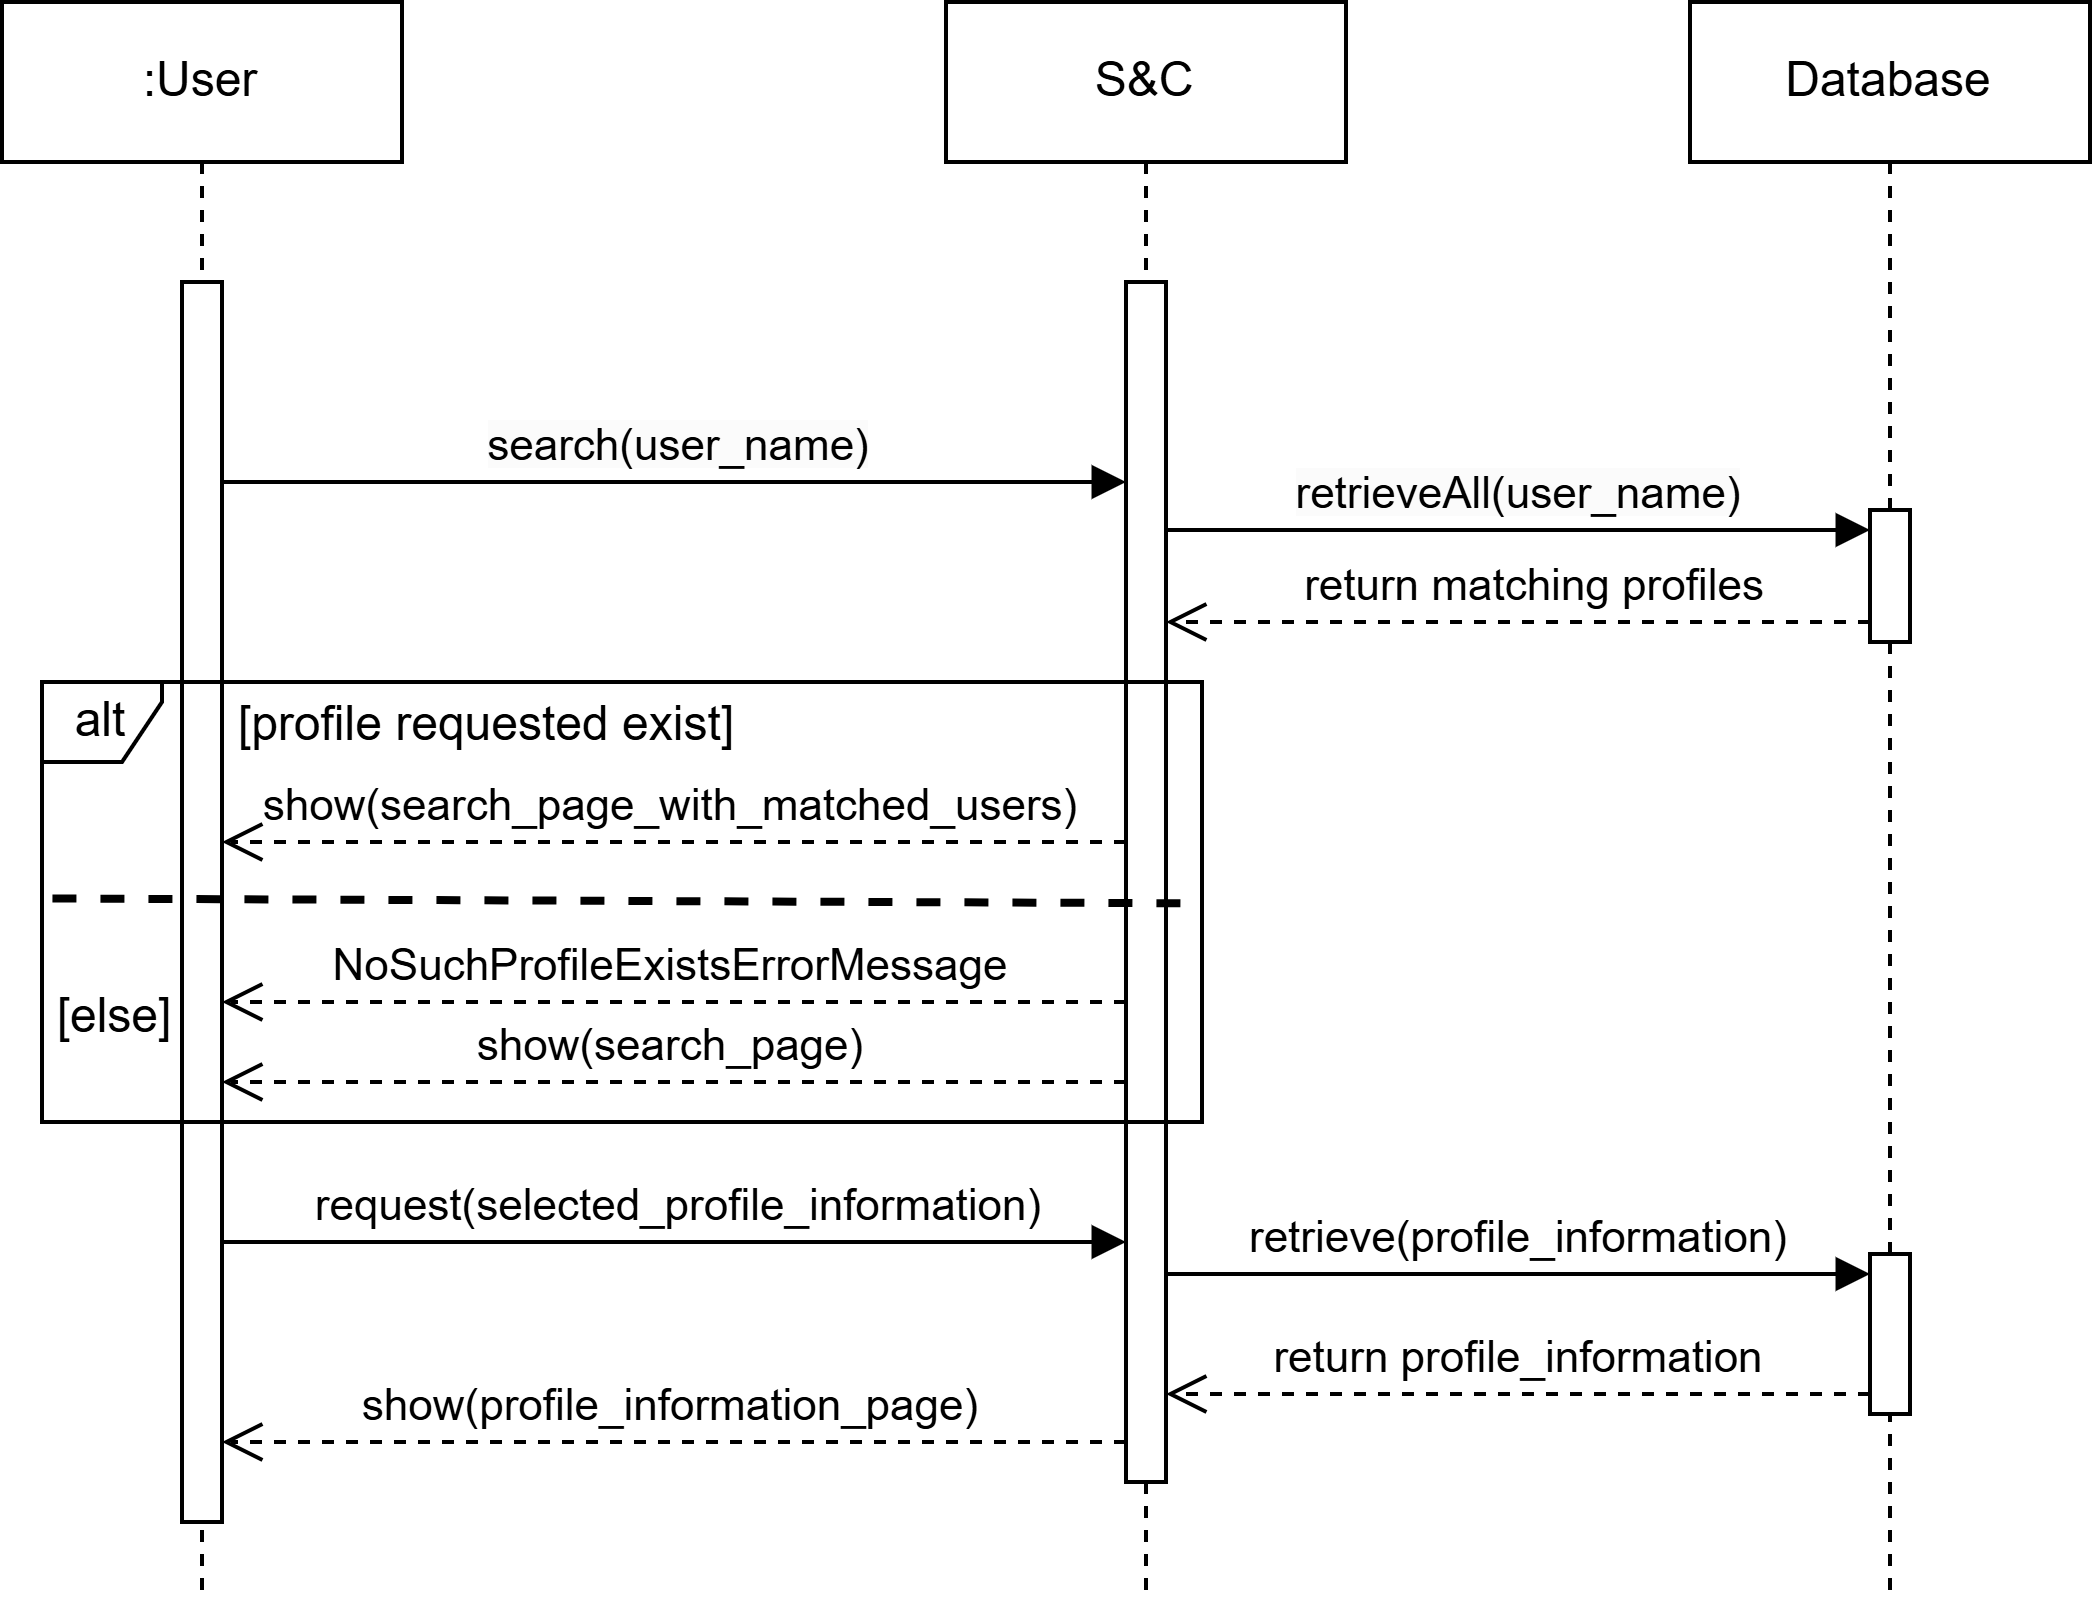
\includegraphics[width=0.75\textwidth]{Images/Sequence_Diagrams/seeProfile_SD.png}
    \caption{User sees profile information Sequence Diagram}
\end{figure}
% Use Case 4
\begin{figure}[H]
    \centering
    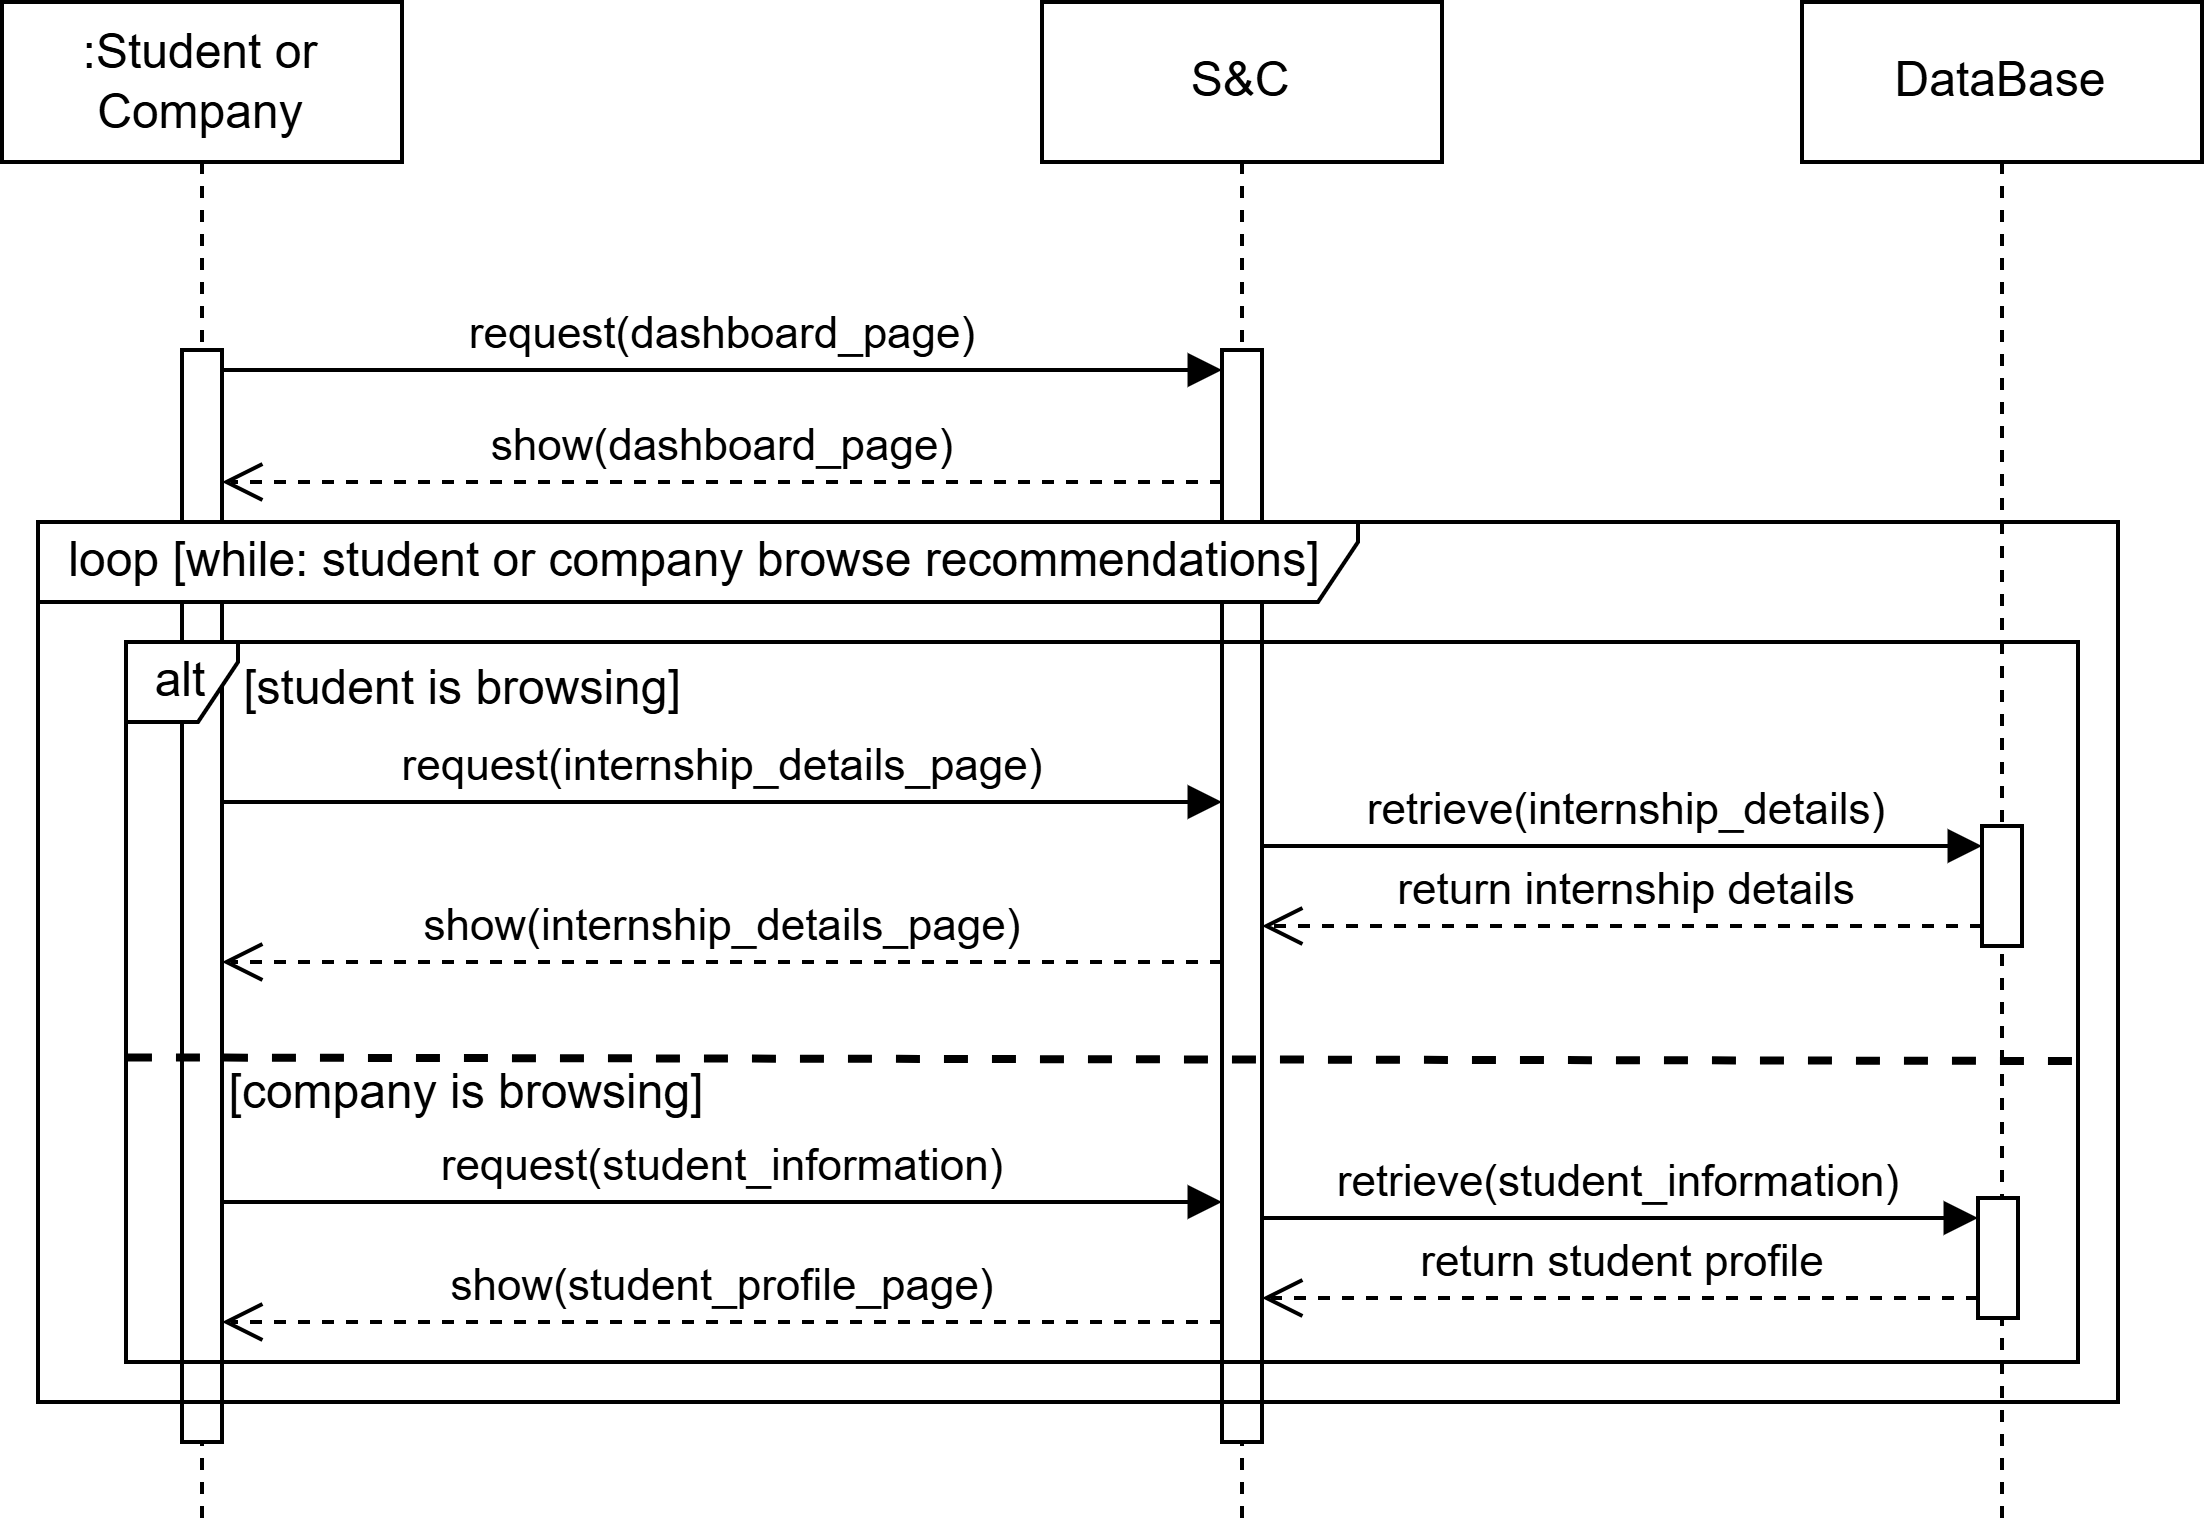
\includegraphics[width=0.8\textwidth]{Images/Sequence_Diagrams/recommendation_SD.png}
    \caption{Student or Company views recommendation Sequence Diagram}
\end{figure}
% Use Case 5
\begin{figure}[H]
    \centering
    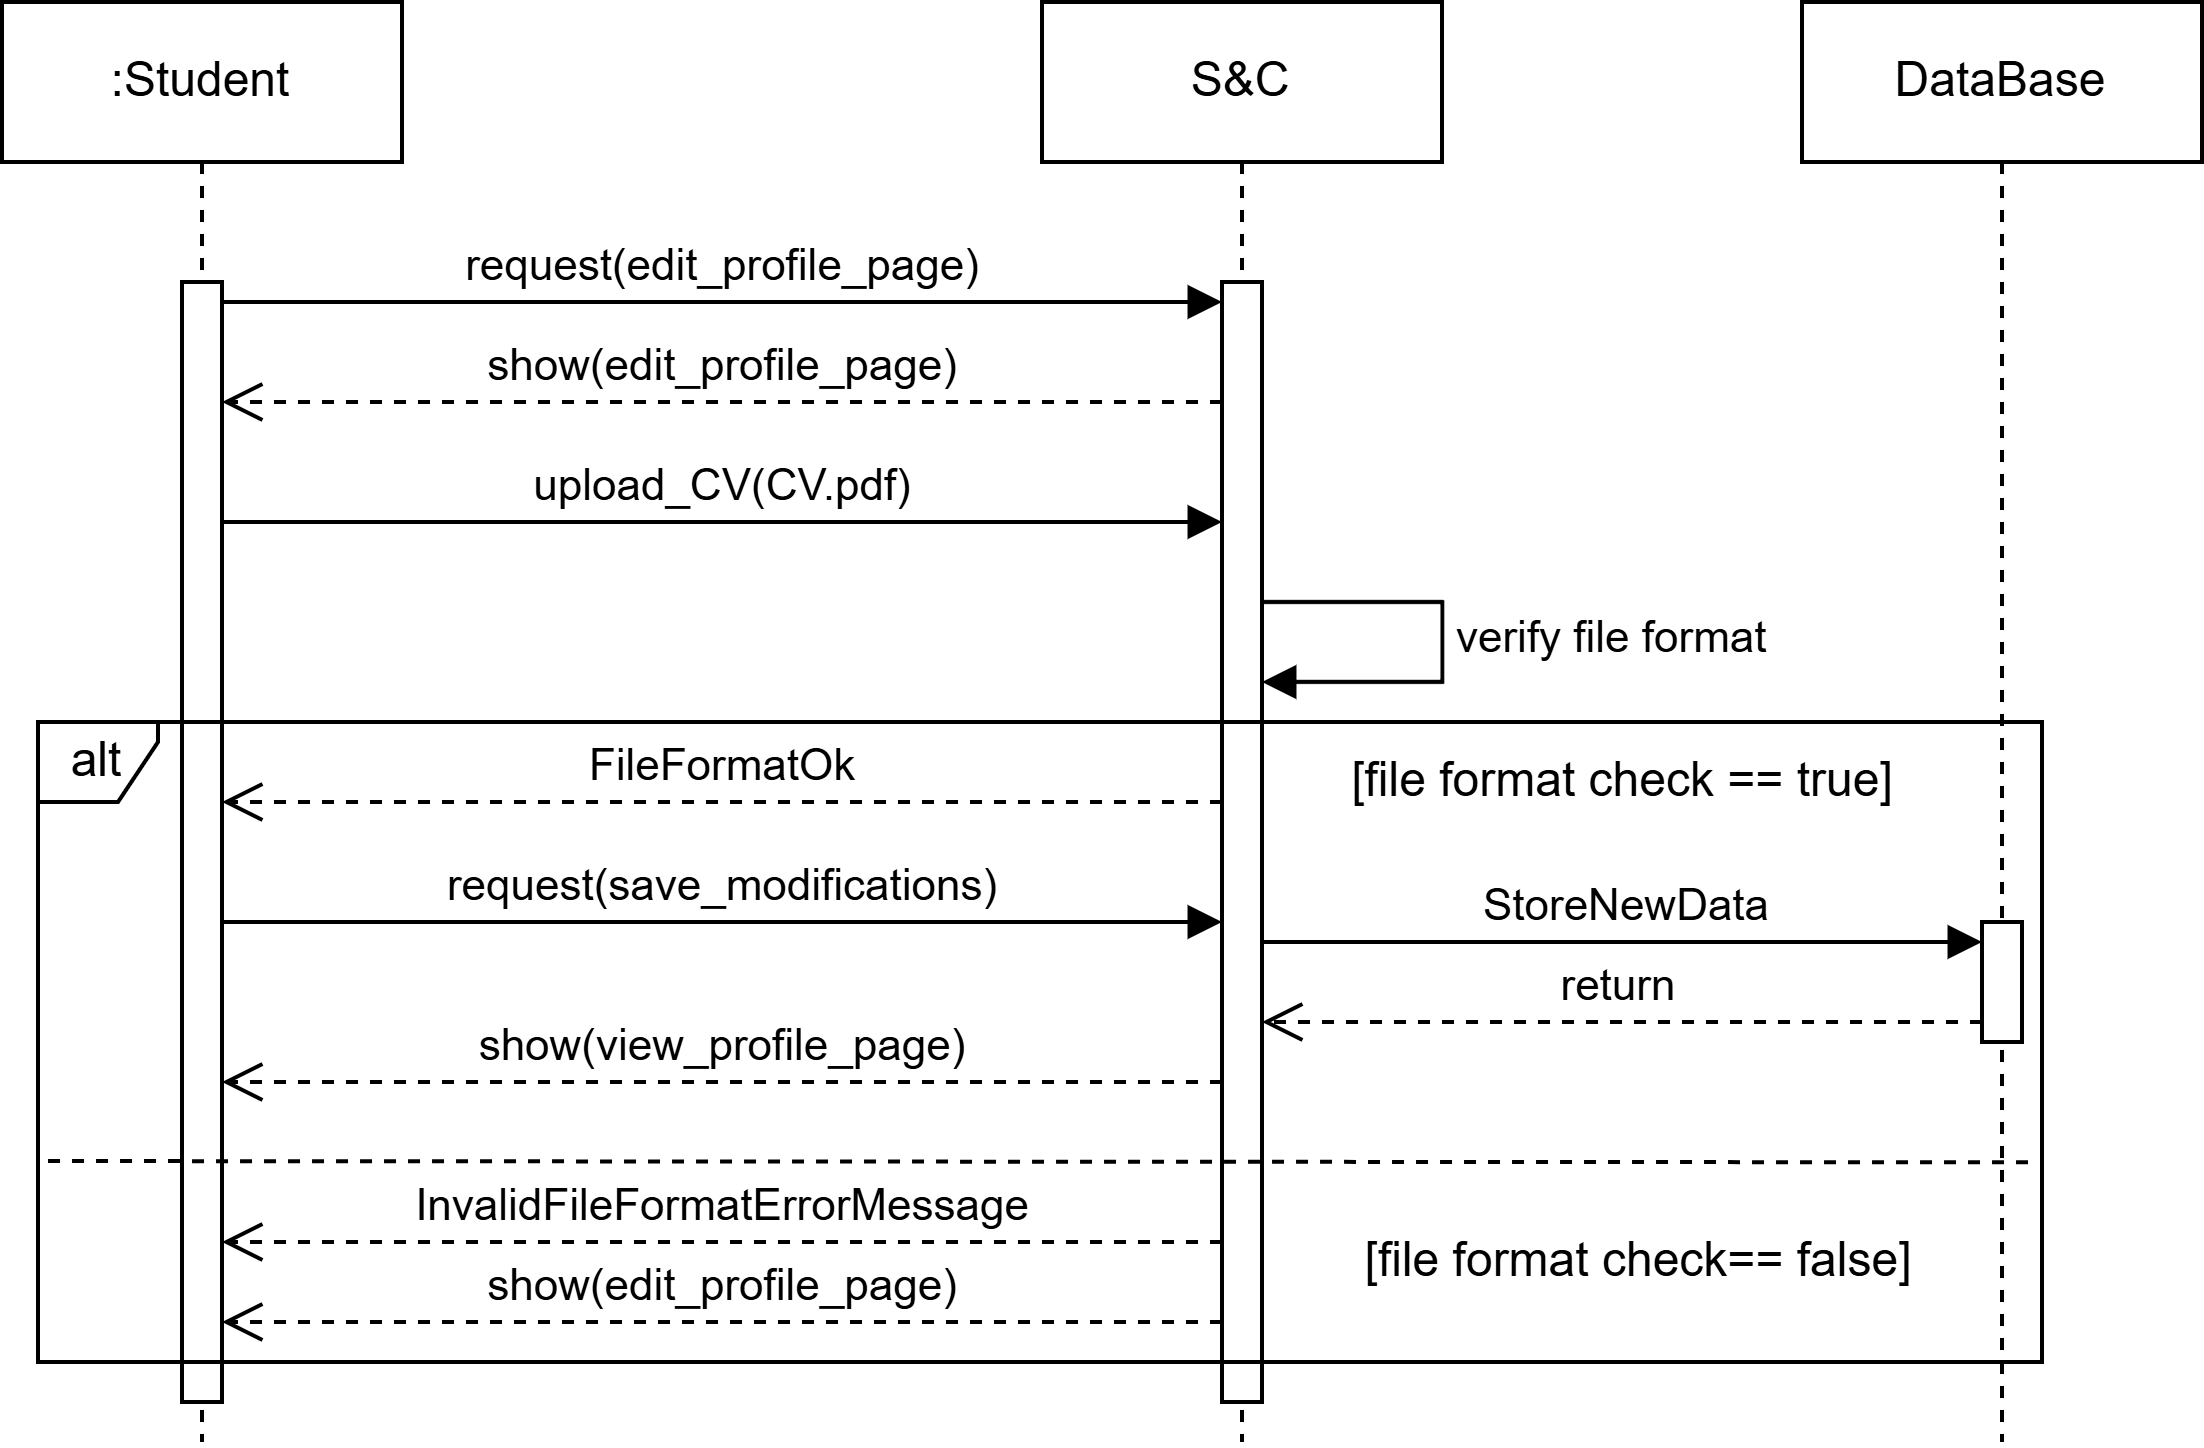
\includegraphics[width=0.8\textwidth]{Images/Sequence_Diagrams/uploadCV_SD.png}
    \caption{Student uploads CV to his profile Sequence Diagram}
\end{figure}
% Use Case 6
\begin{figure}[H]
    \centering
    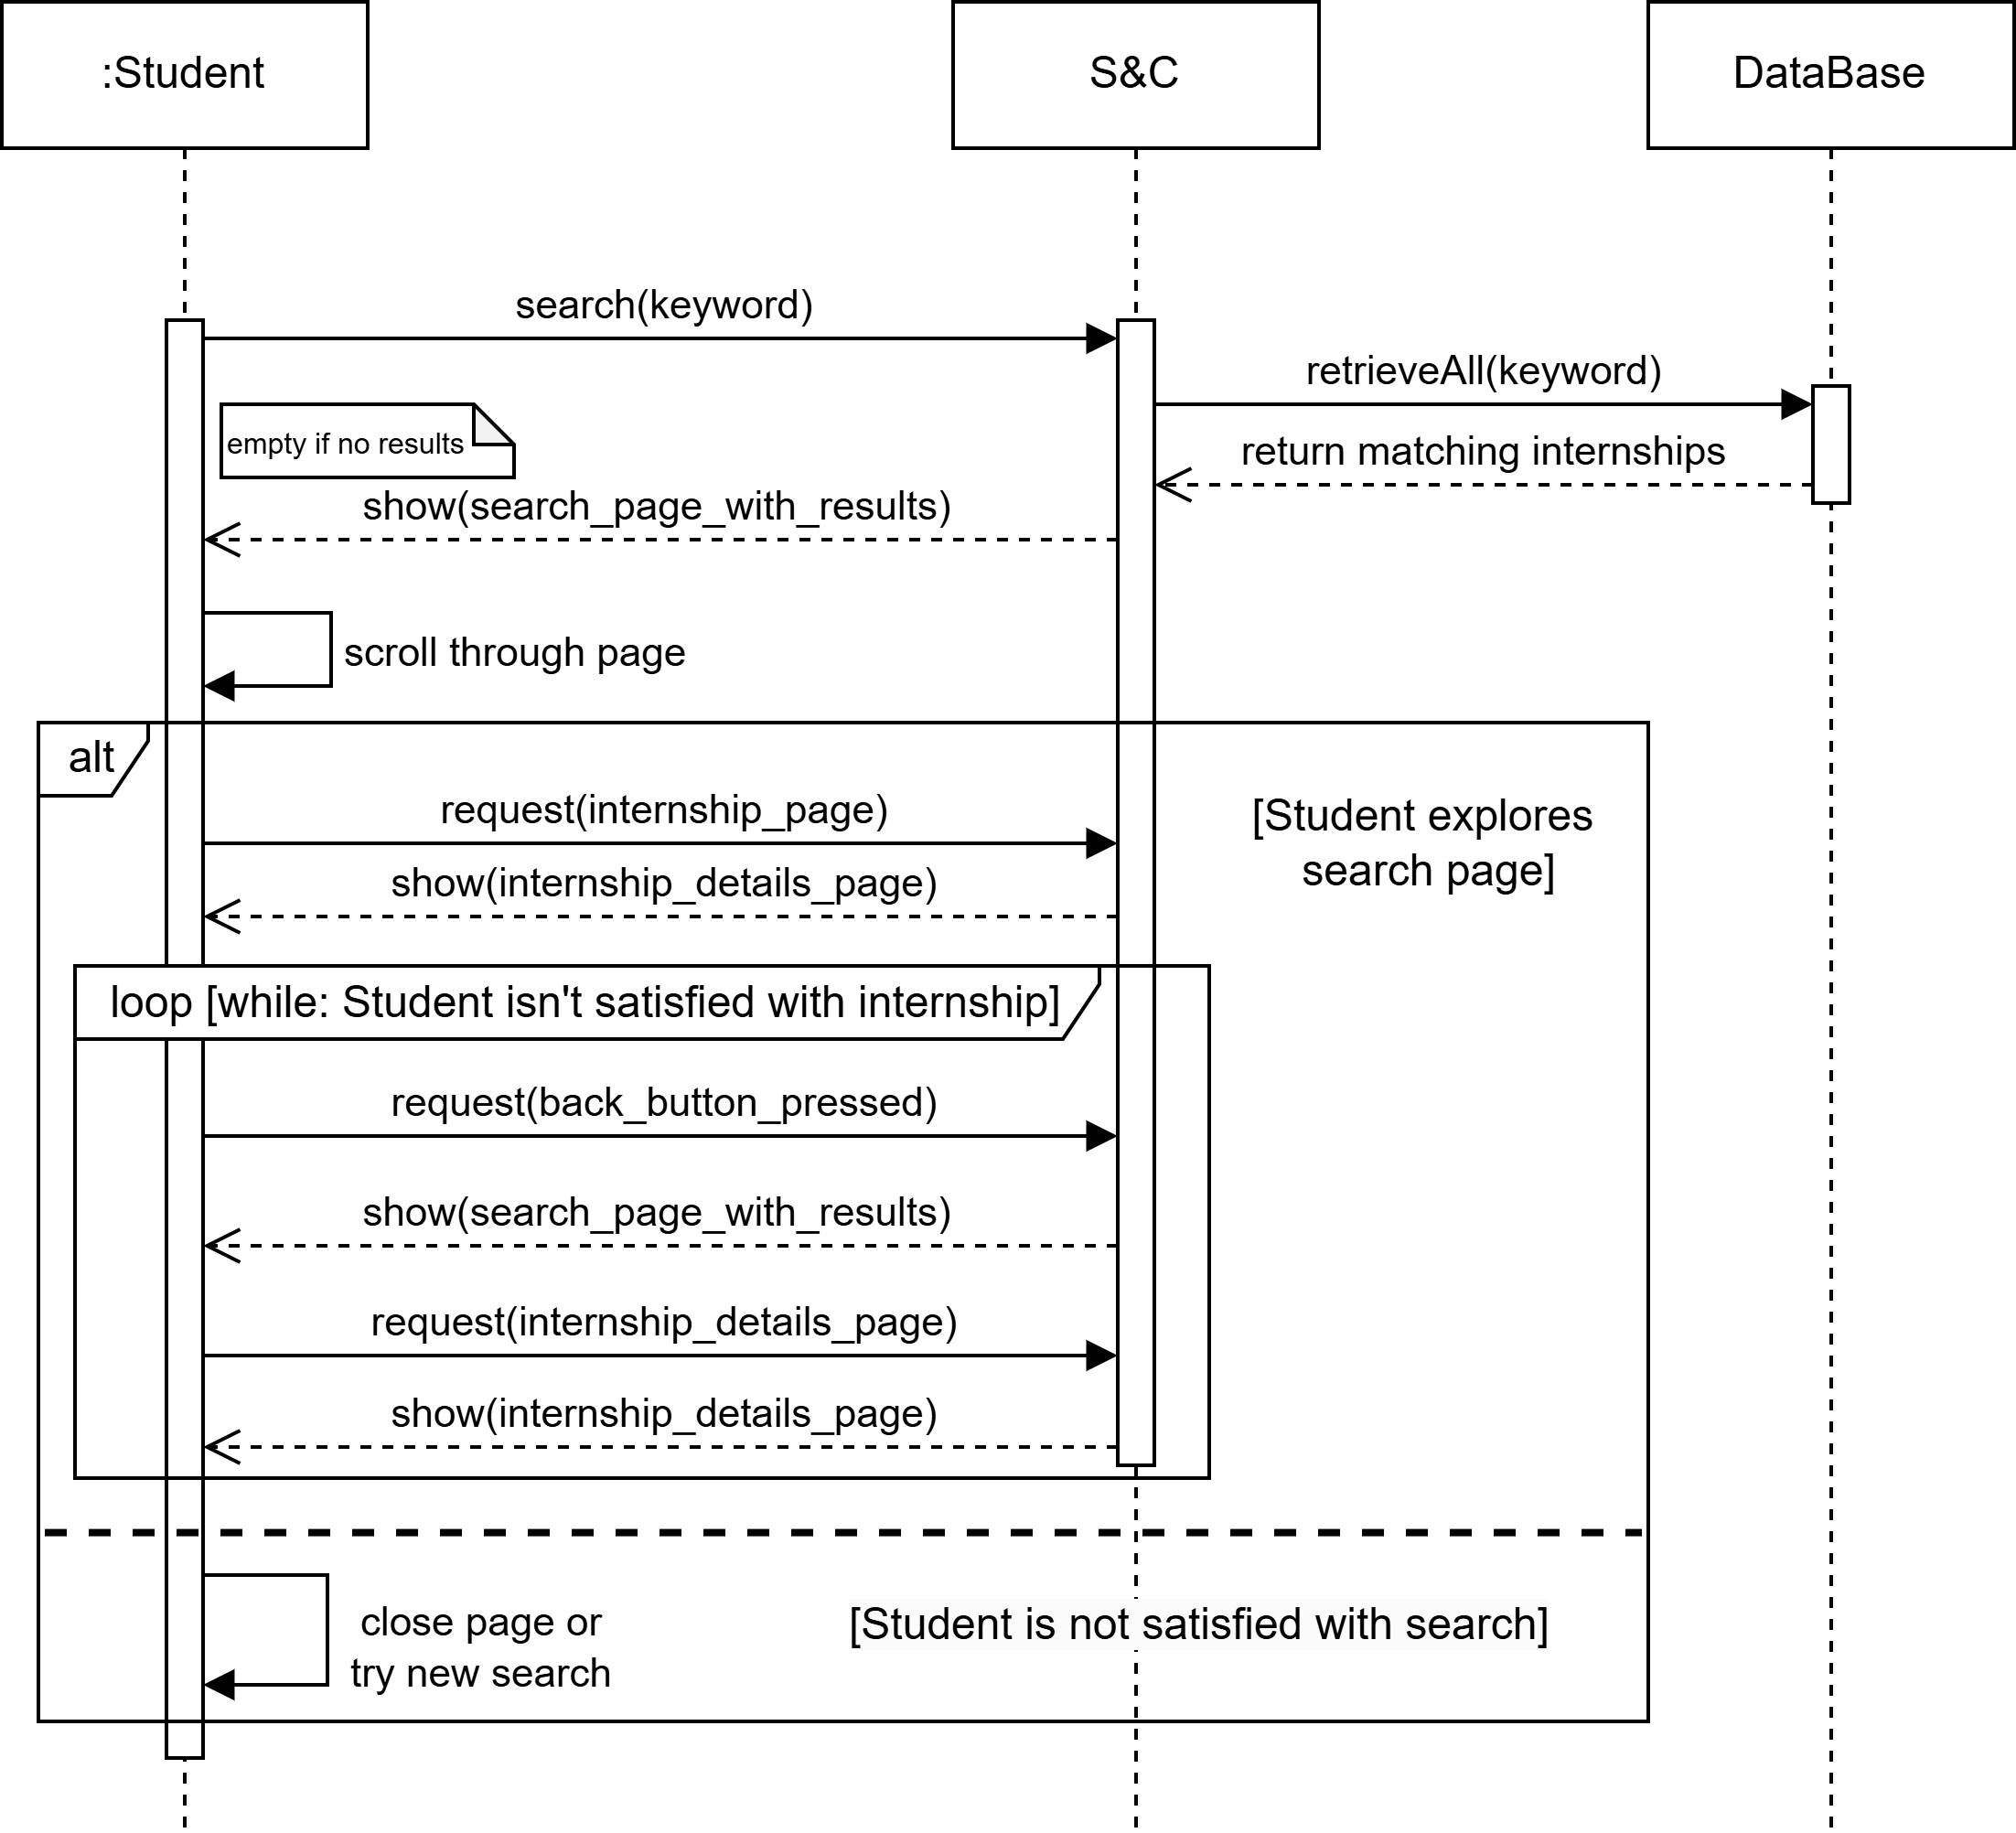
\includegraphics[width=0.75\textwidth]{Images/Sequence_Diagrams/searchInt_SD.png}
    \caption{Student searches for an internship Sequence Diagram}
\end{figure}
% Use Case 7
\begin{figure}[H]
    \centering
    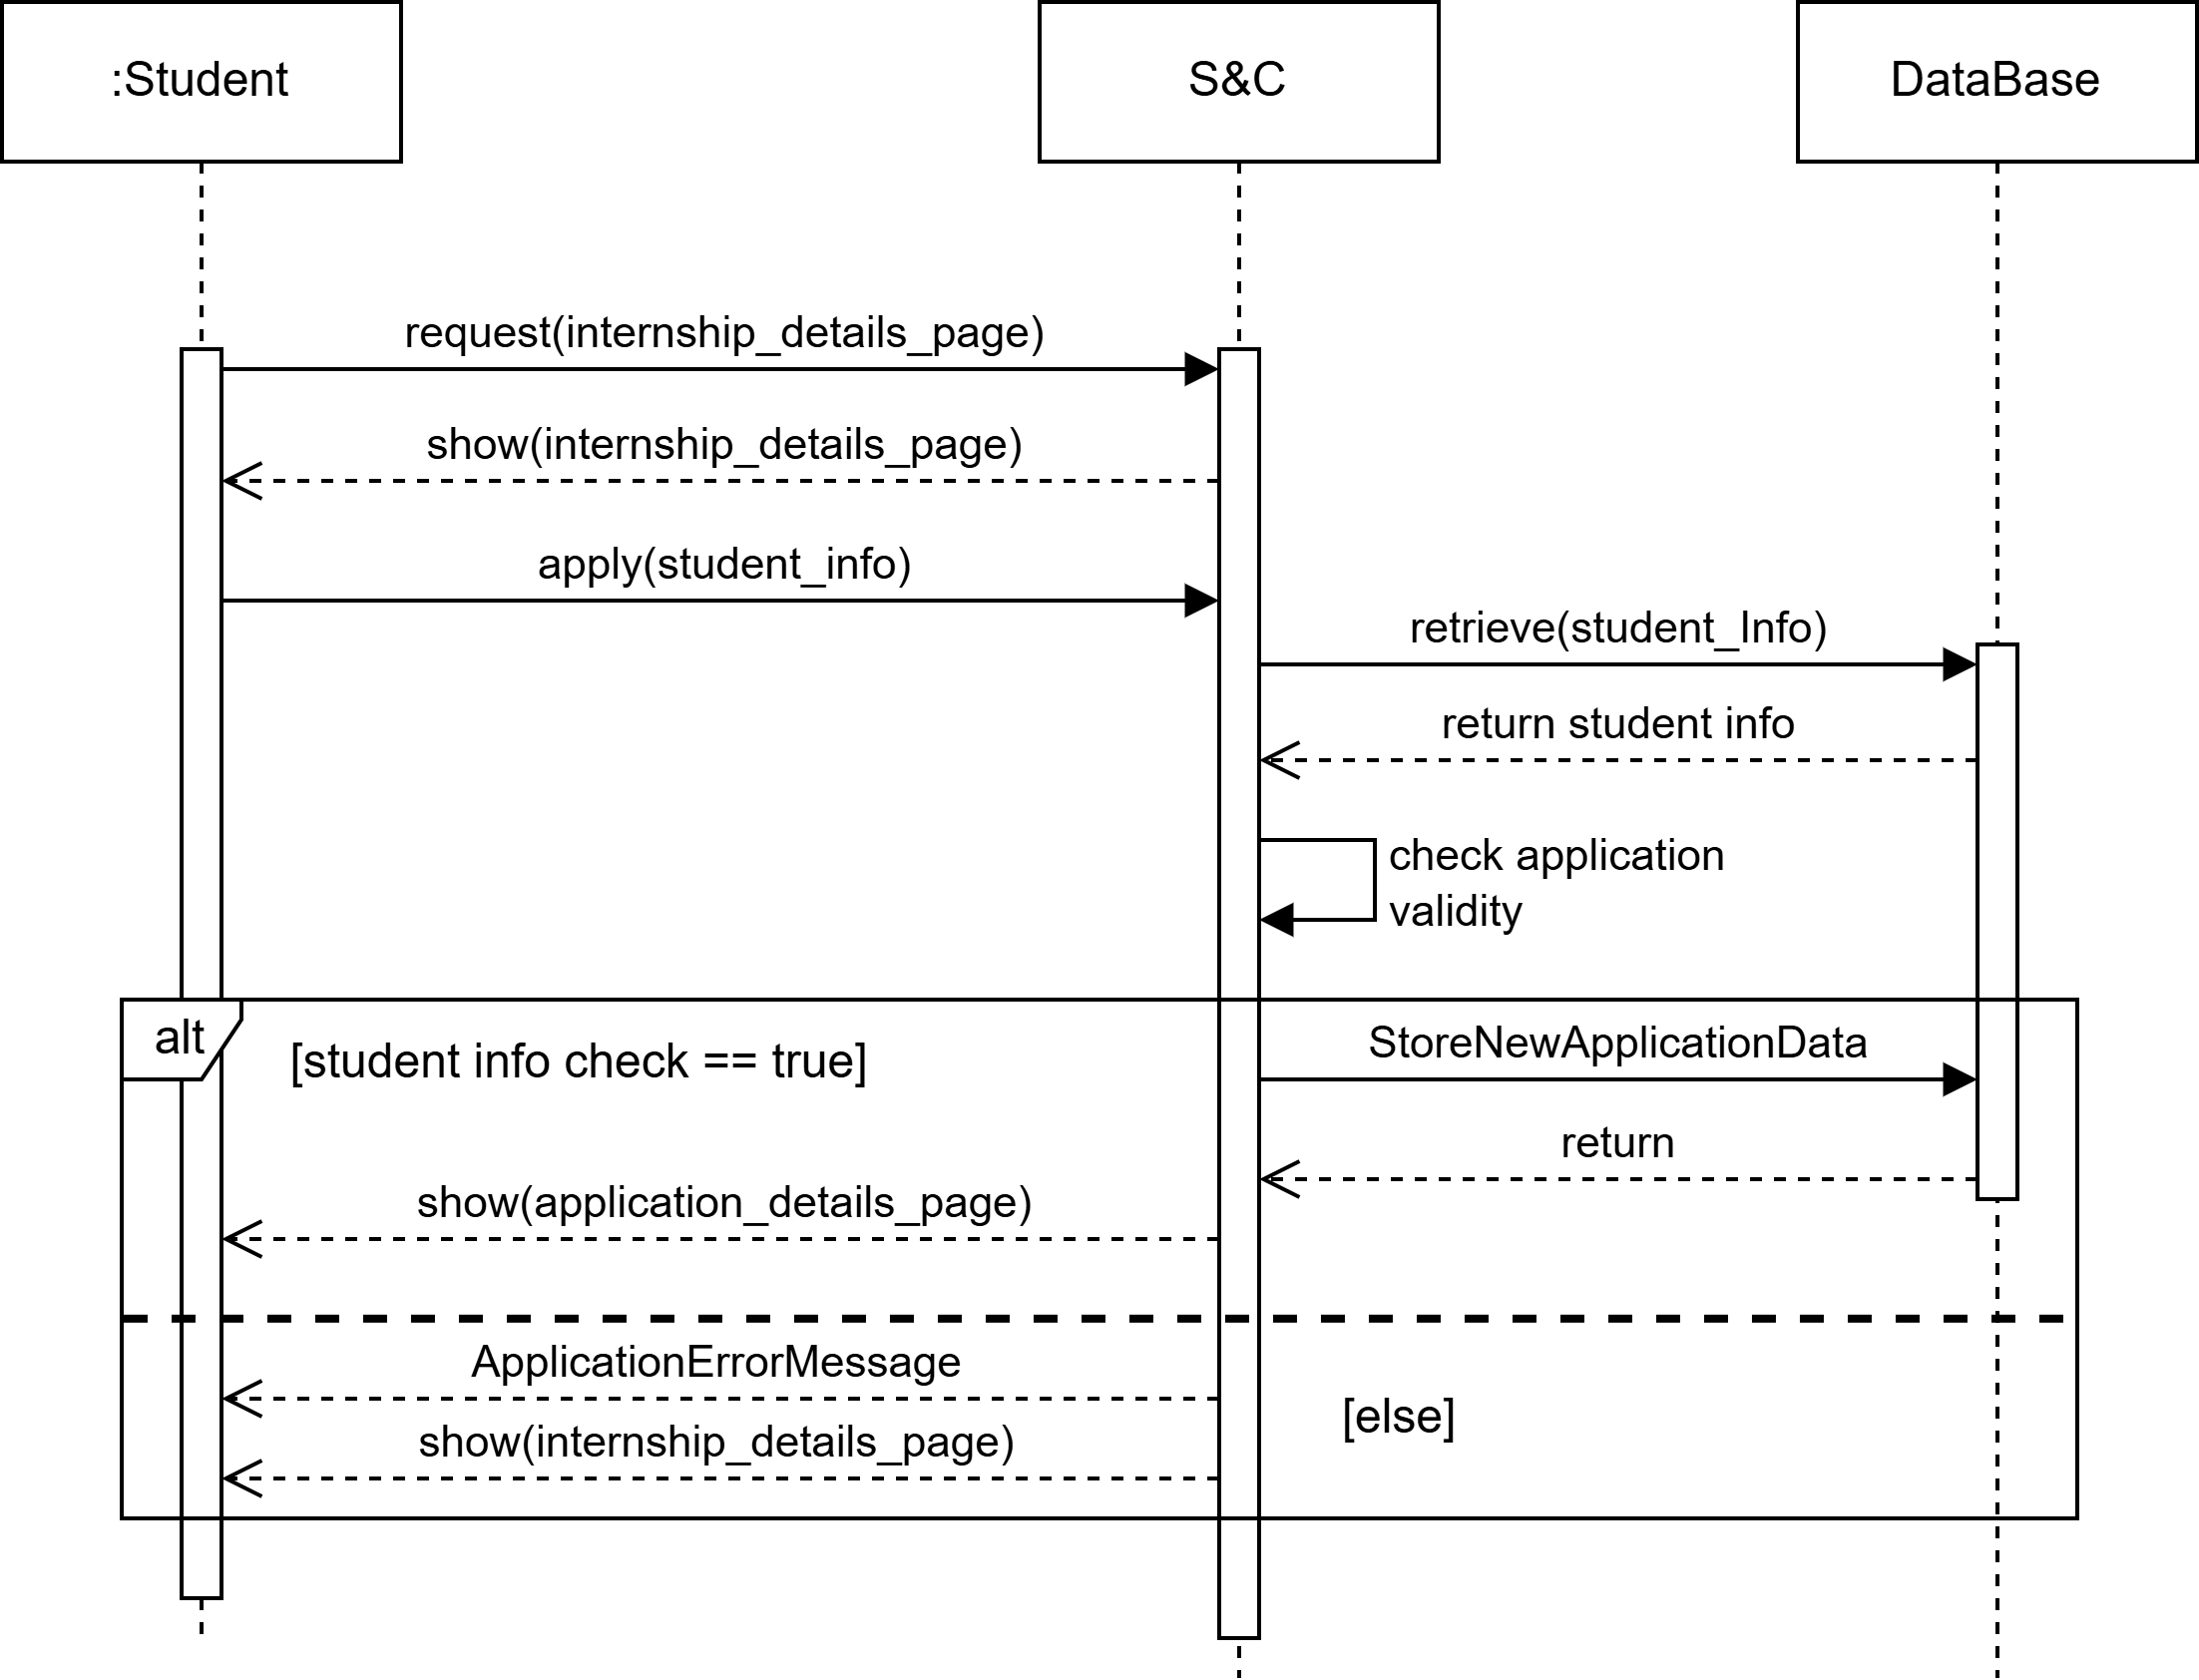
\includegraphics[width=0.75\textwidth]{Images/Sequence_Diagrams/applyInt_SD.png}
    \caption{Student applies for an internship Sequence Diagram}
\end{figure}
% Use Case 8
\begin{figure}[H]
    \centering
    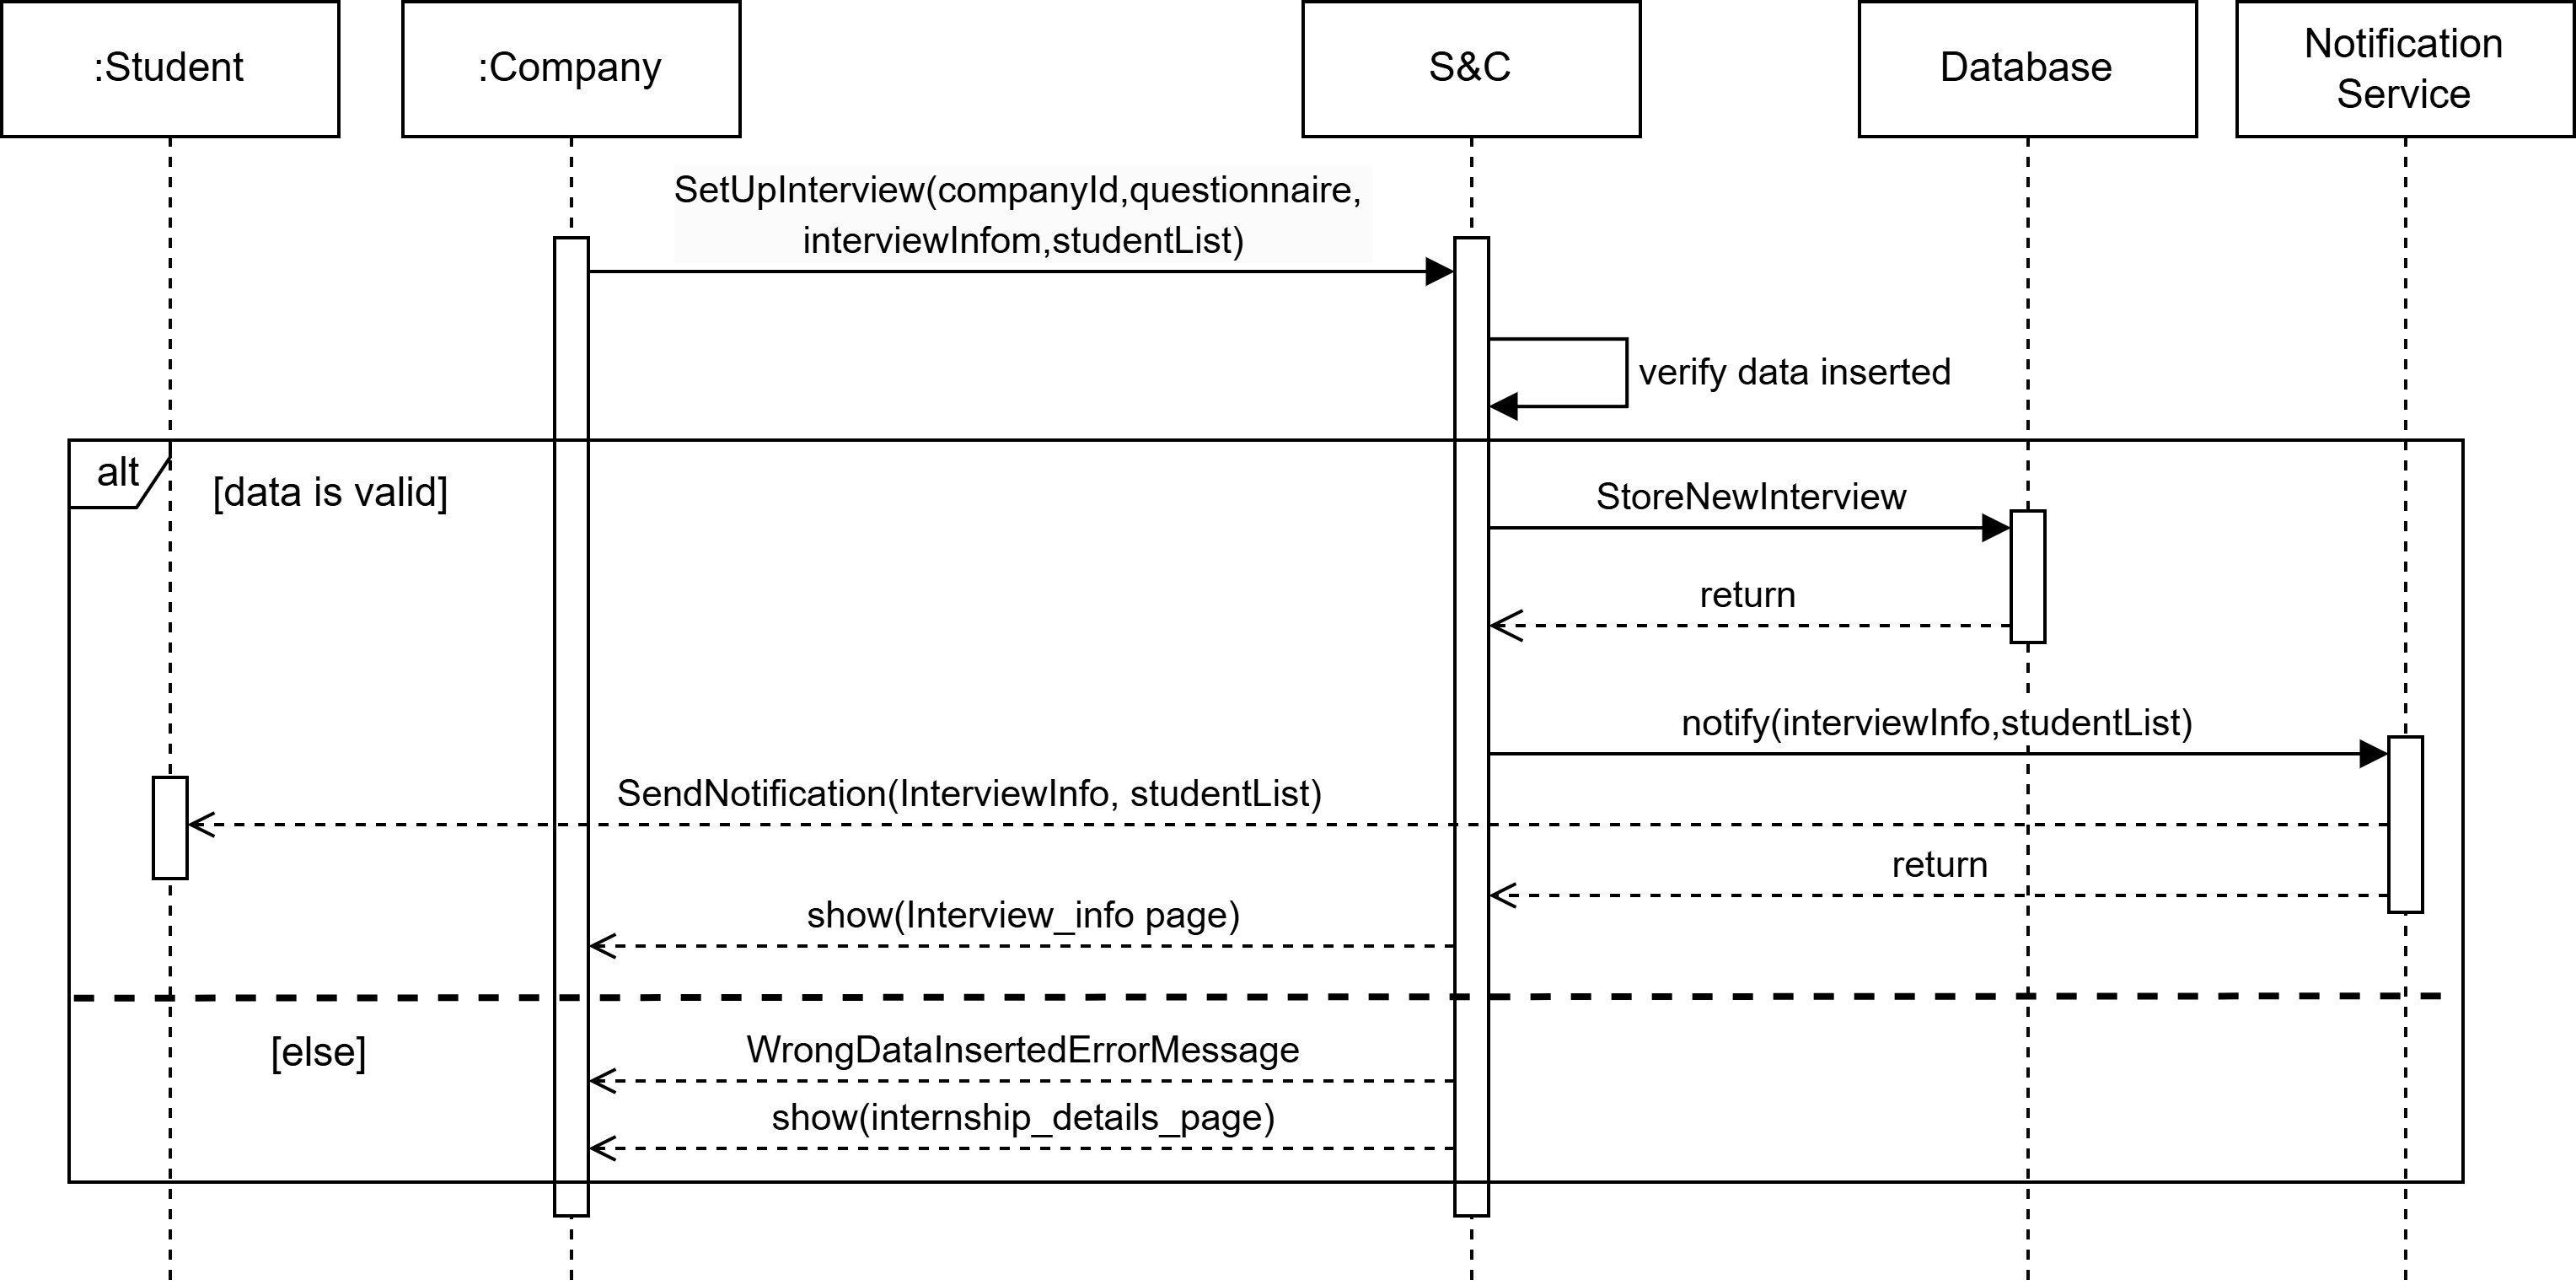
\includegraphics[width=0.9\textwidth]{Images/Sequence_Diagrams/createIntvw_SD.png}
    \caption{Company creates an interview Sequence Diagram}
\end{figure}
% Use Case 9
\begin{figure}[H]
    \centering
    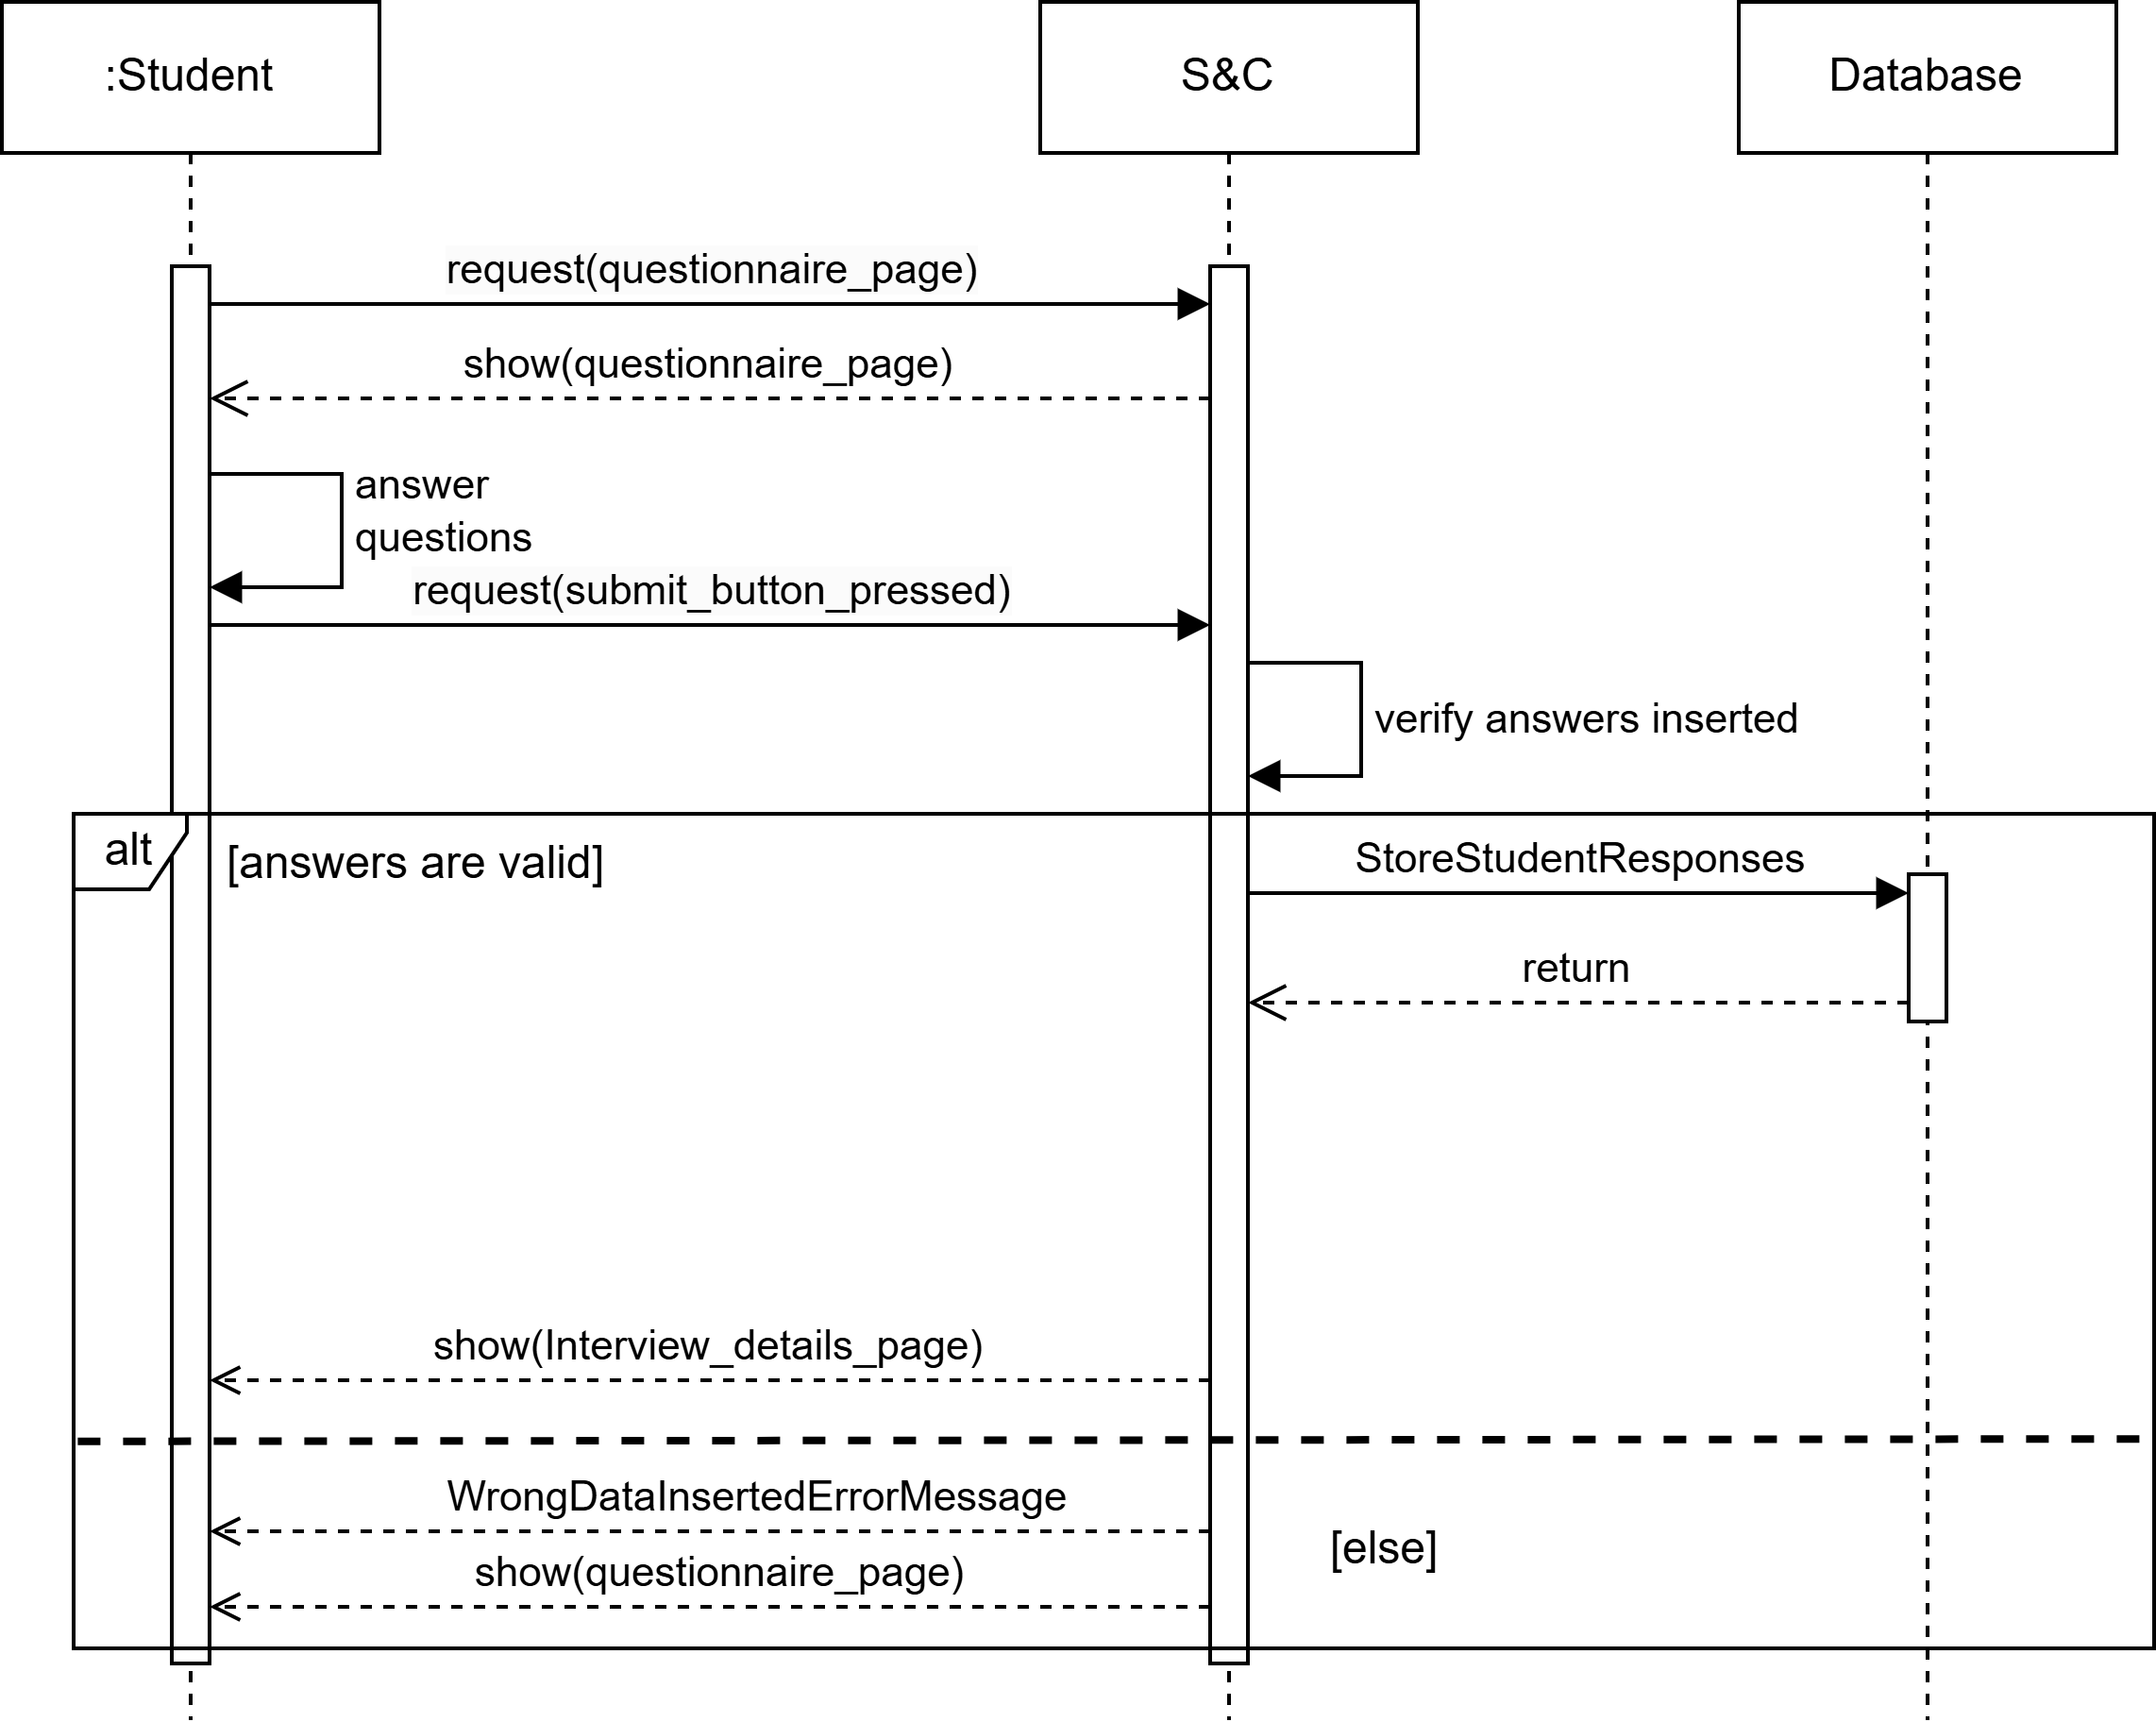
\includegraphics[width=0.9\textwidth]{Images/Sequence_Diagrams/respondQuest_SD.png}
    \caption{Student responds to an interview questionnaire Sequence Diagram}
\end{figure}
% Use Case 10
\begin{figure}[H]
    \centering
    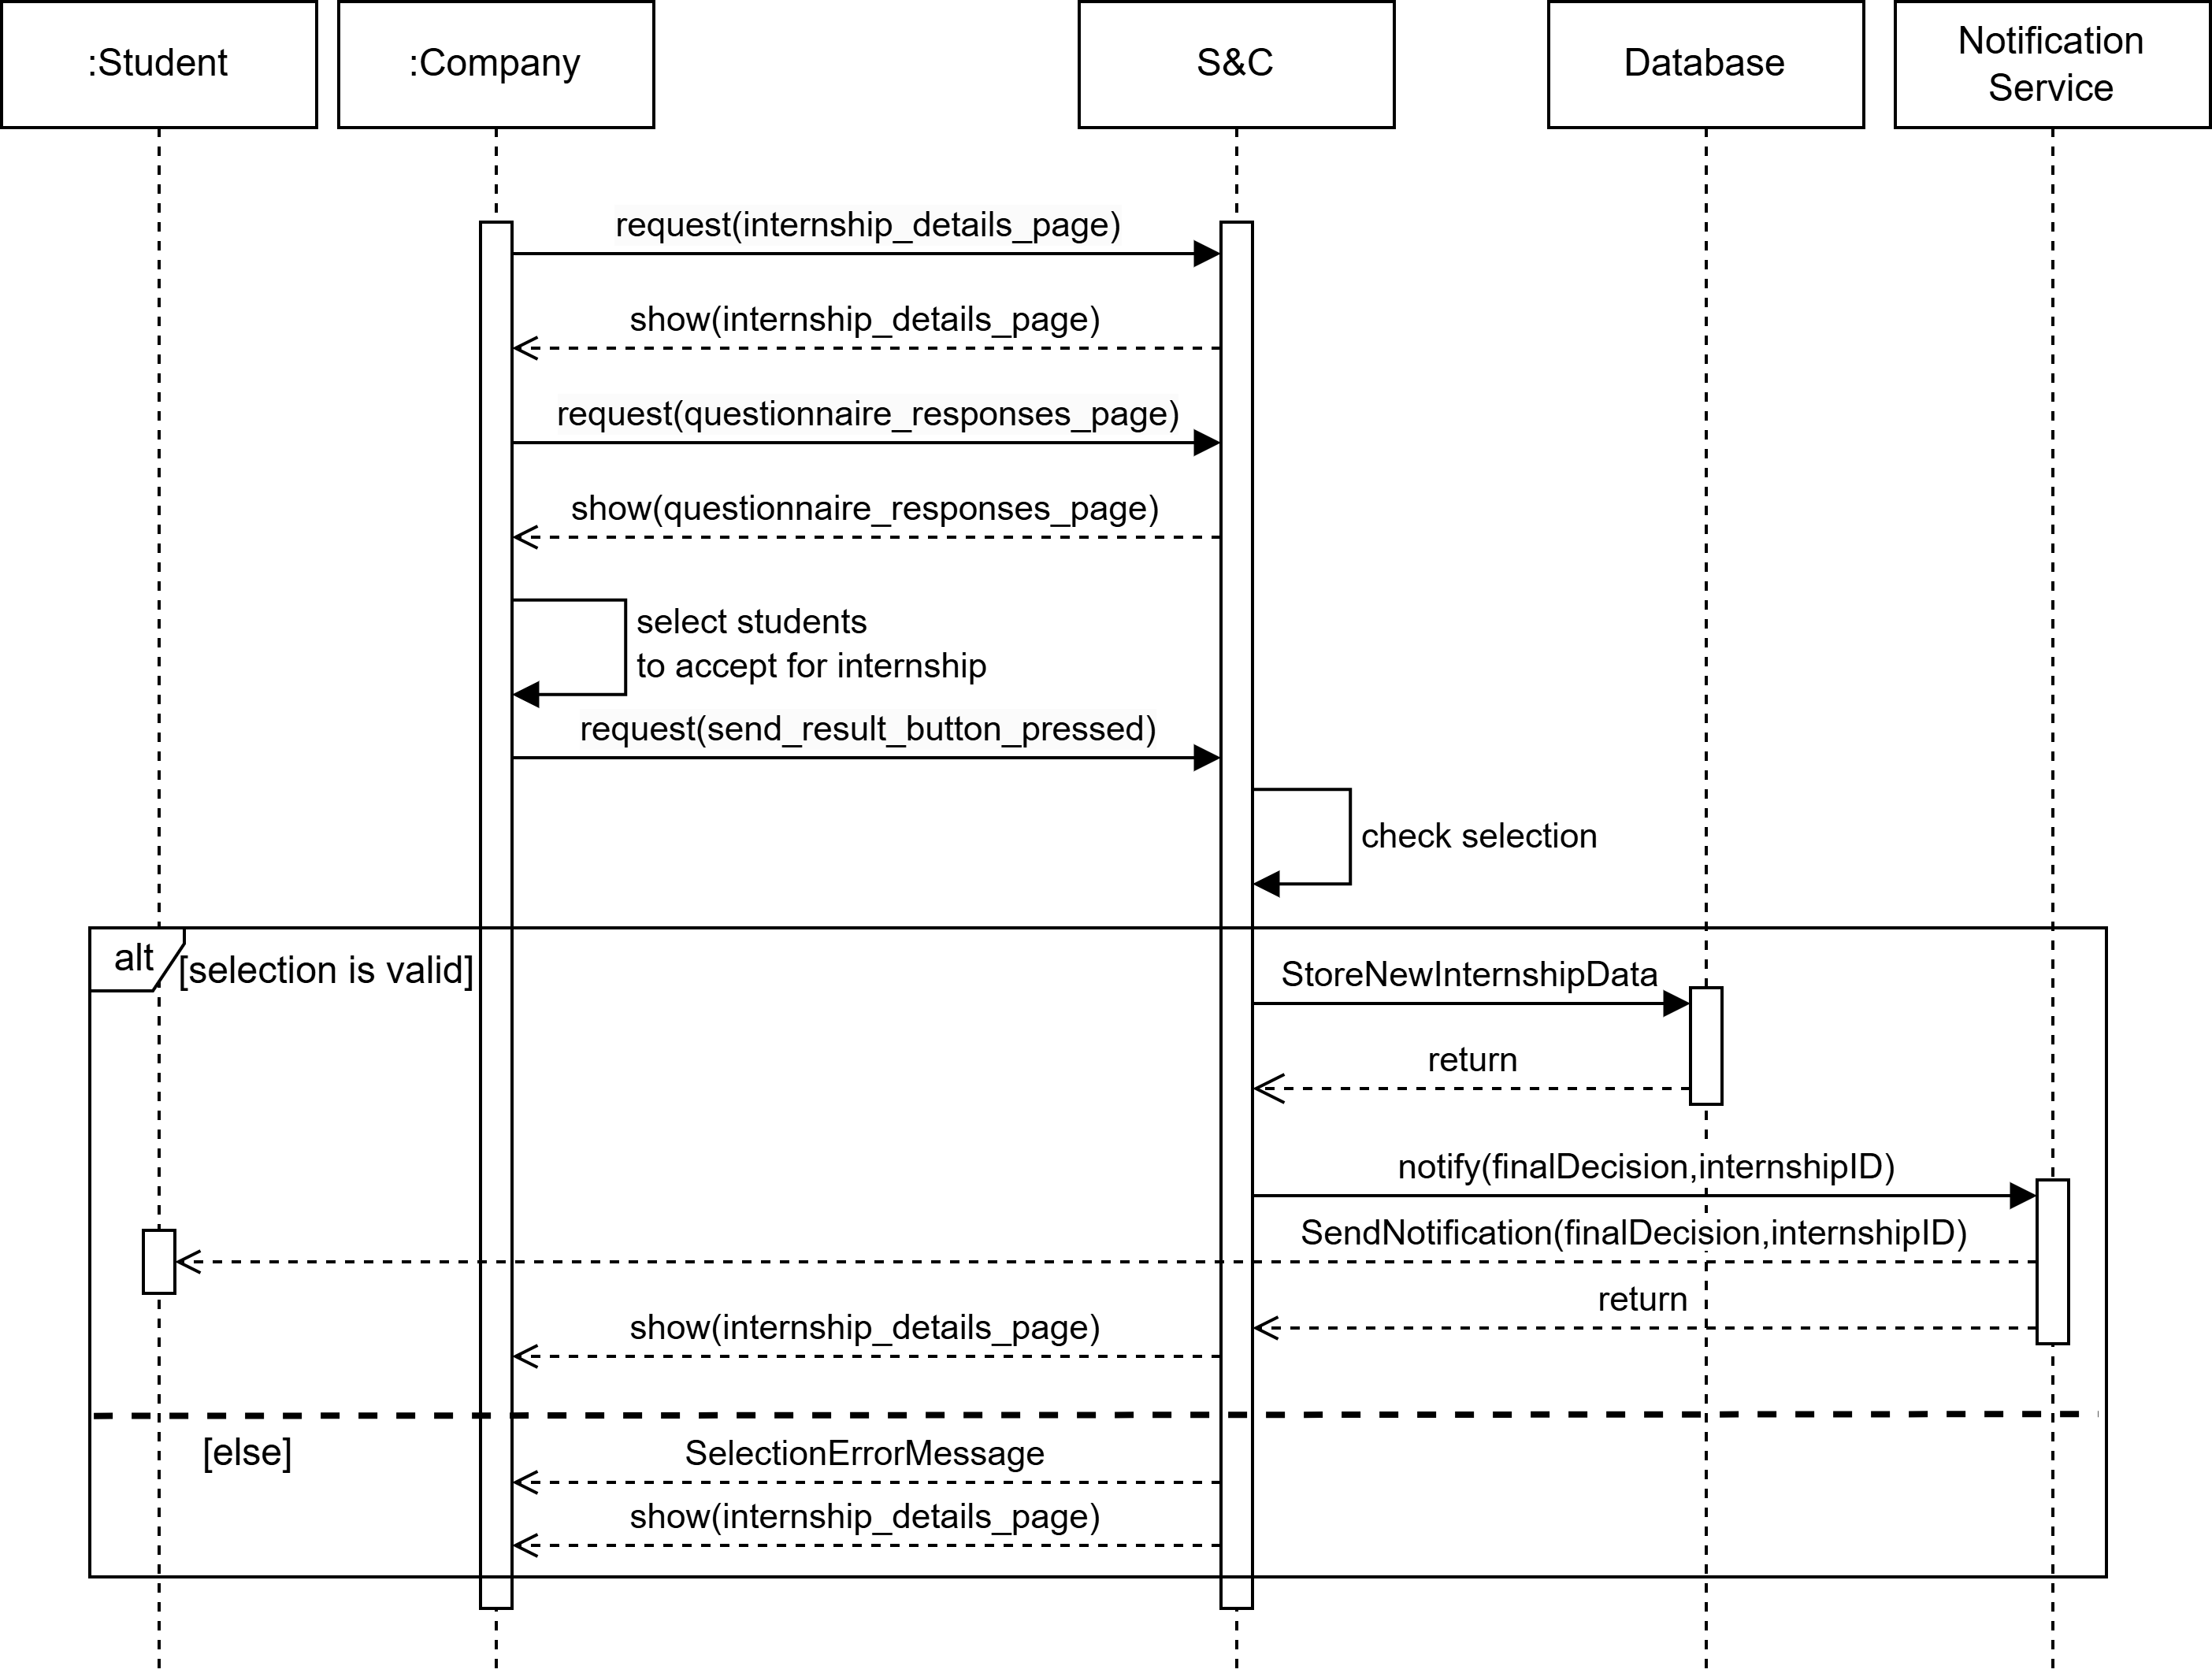
\includegraphics[width=0.9\textwidth]{Images/Sequence_Diagrams/intResults_SD.png}
    \caption{Company sends interview results Sequence Diagram}
\end{figure}
% Use Case 11
\begin{figure}[H]
    \centering
    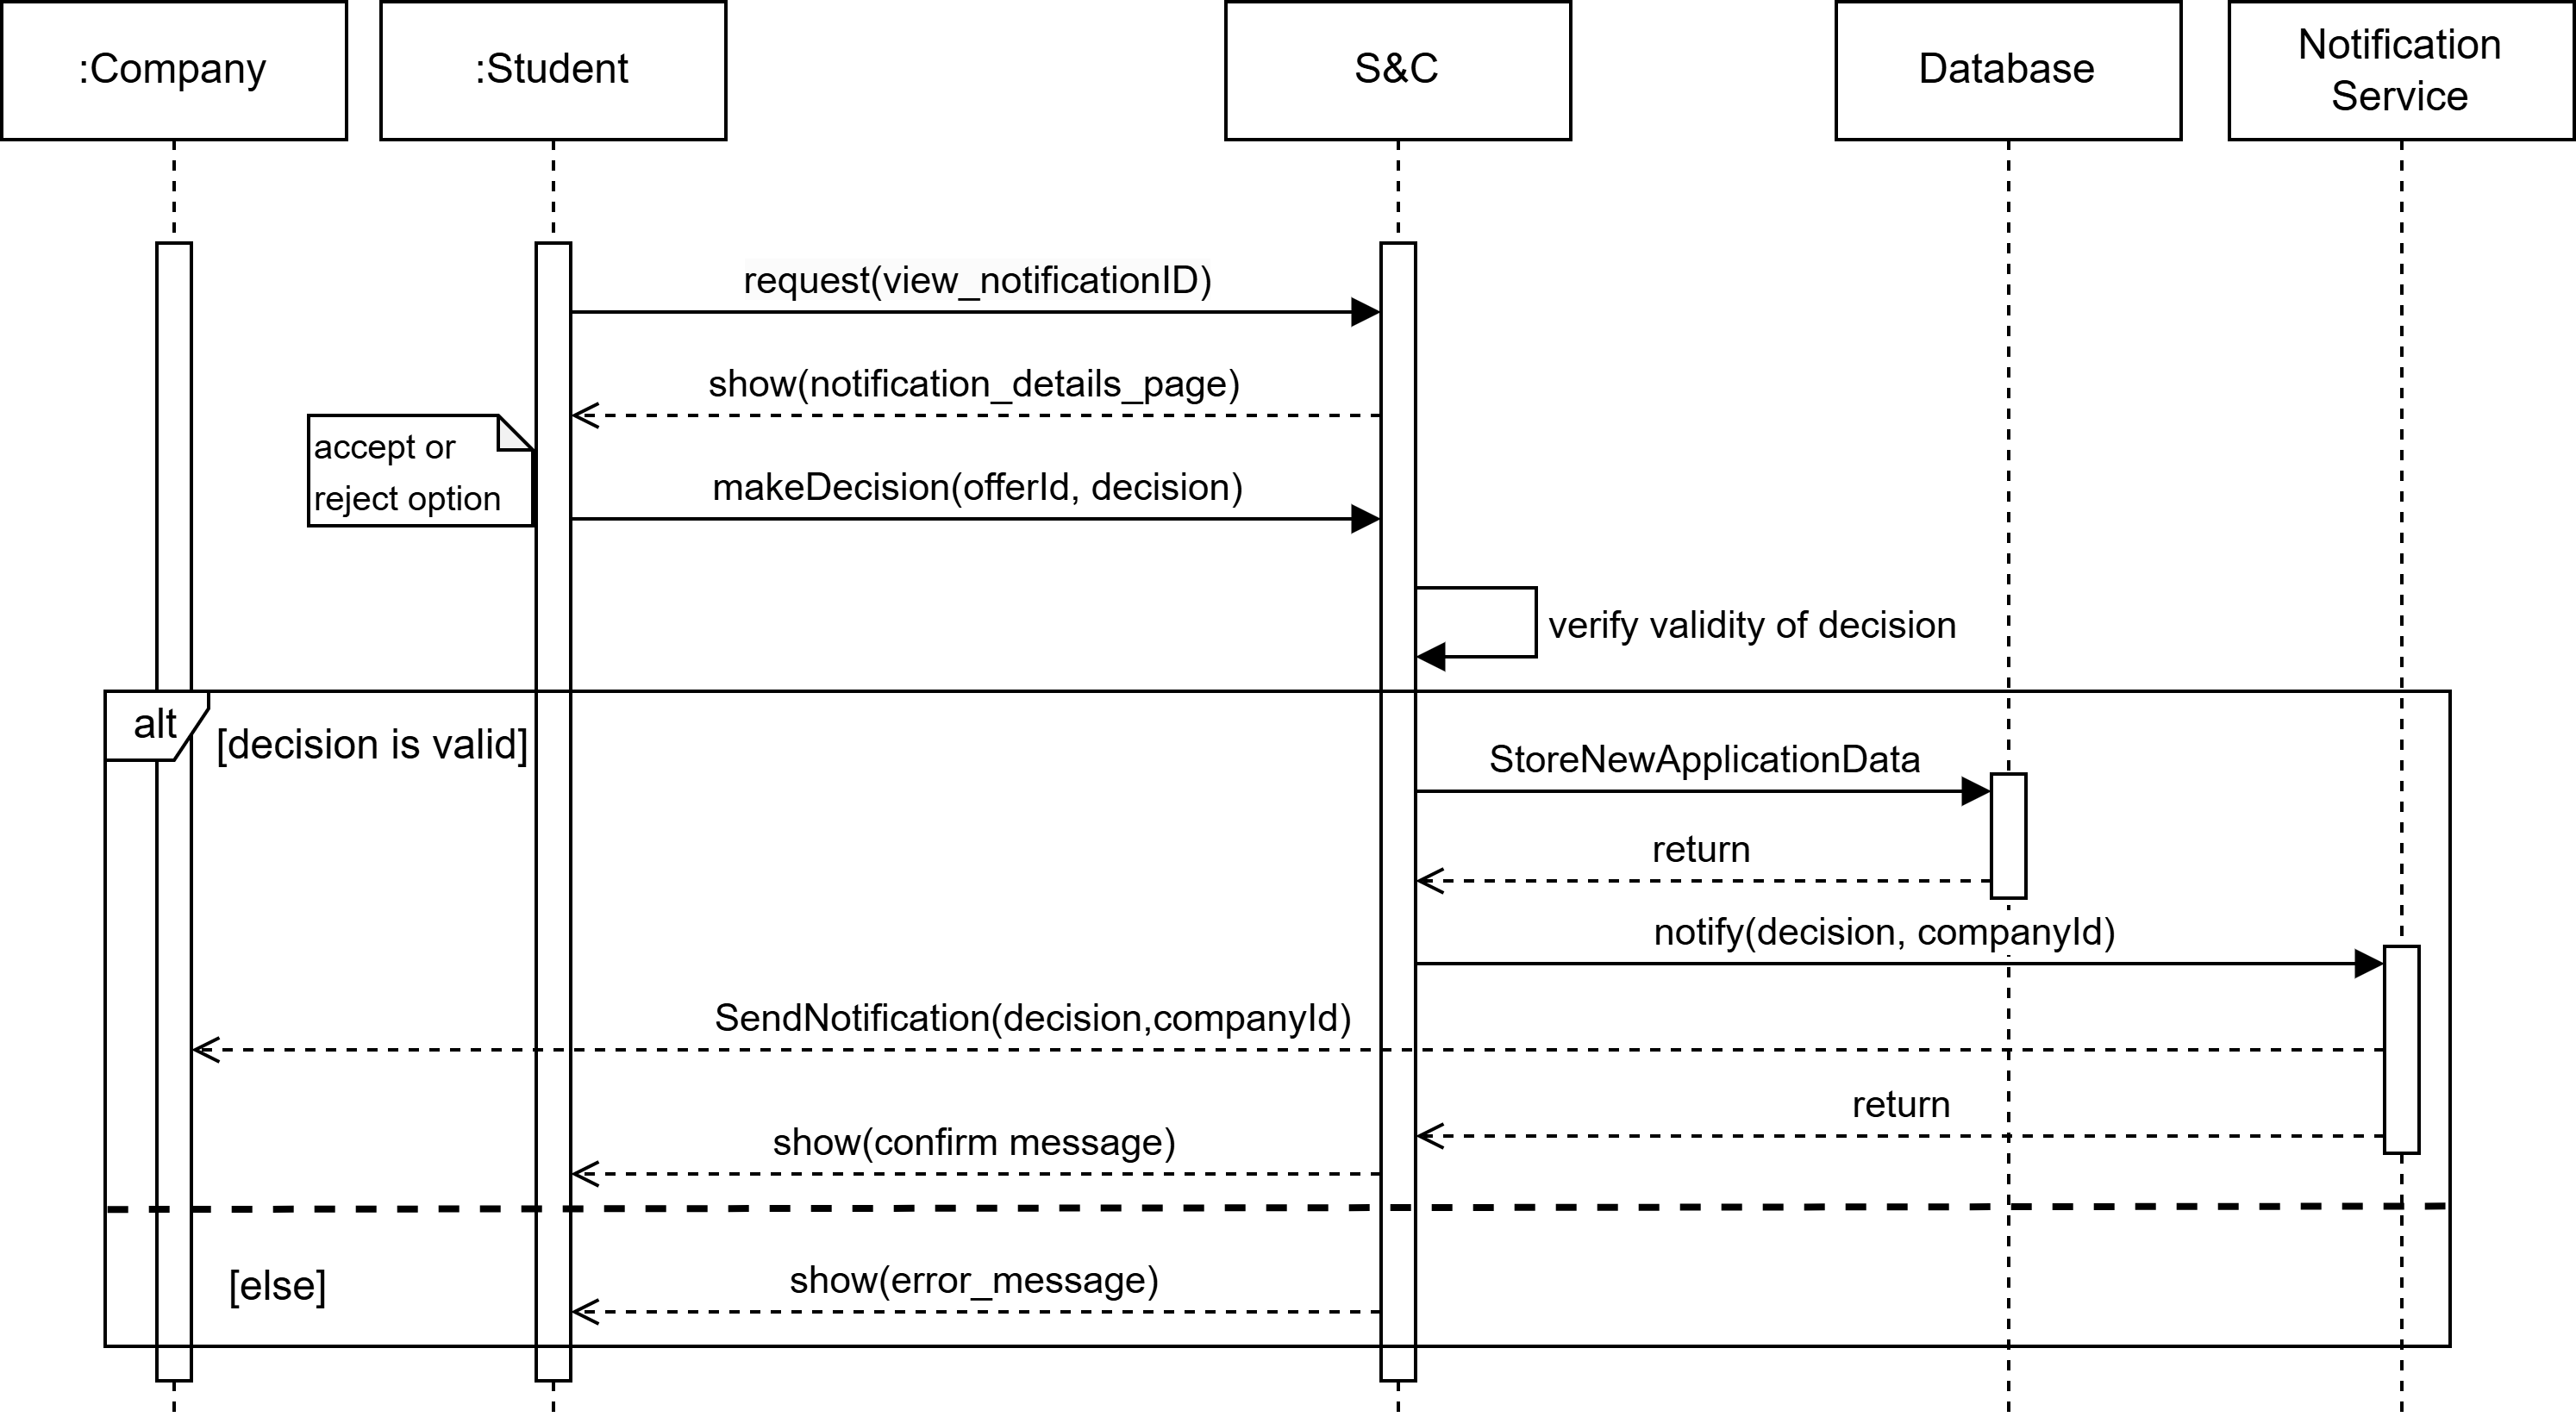
\includegraphics[width=1\textwidth]{Images/Sequence_Diagrams/acceptRej_SD.png}
    \caption{Student accepts/rejects an offer Sequence Diagram}
\end{figure}
% Use Case 12
\begin{figure}[H]
    \centering
    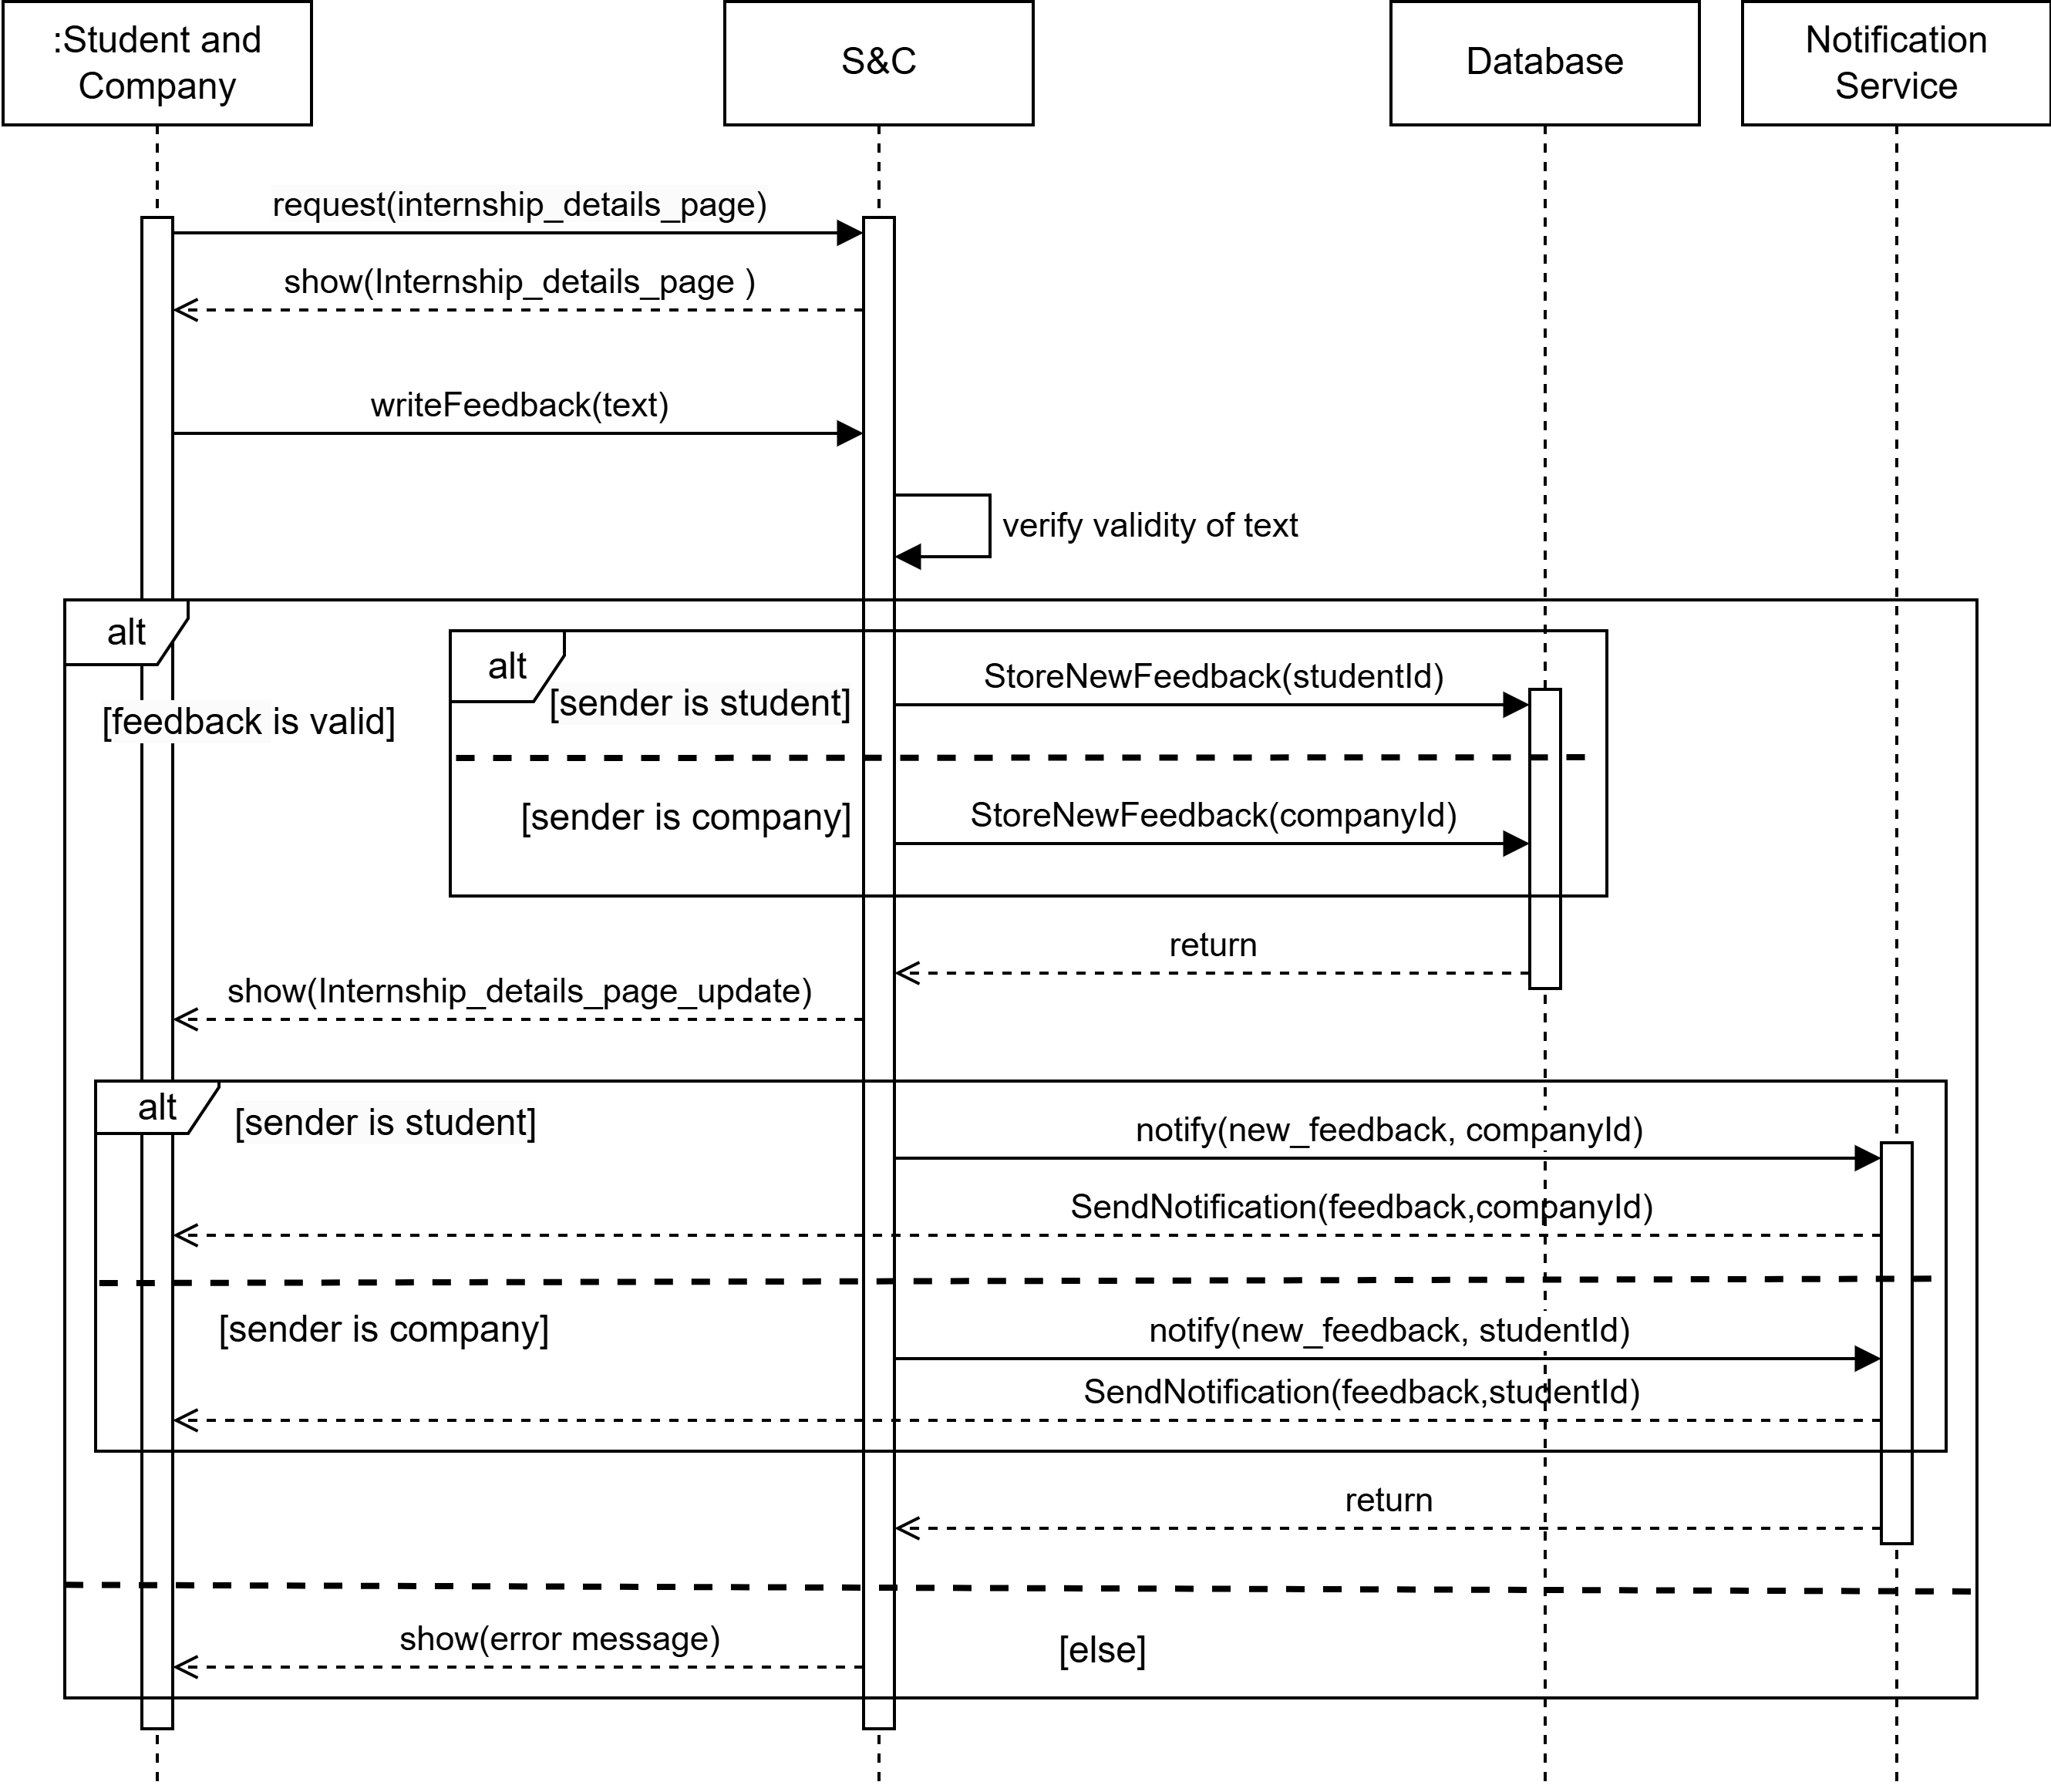
\includegraphics[width=1\textwidth]{Images/Sequence_Diagrams/feedback_SD.png}
    \caption{Student or Company writes feedback Sequence Diagram}
\end{figure}
% Use Case 13
\begin{figure}[H]
    \centering
    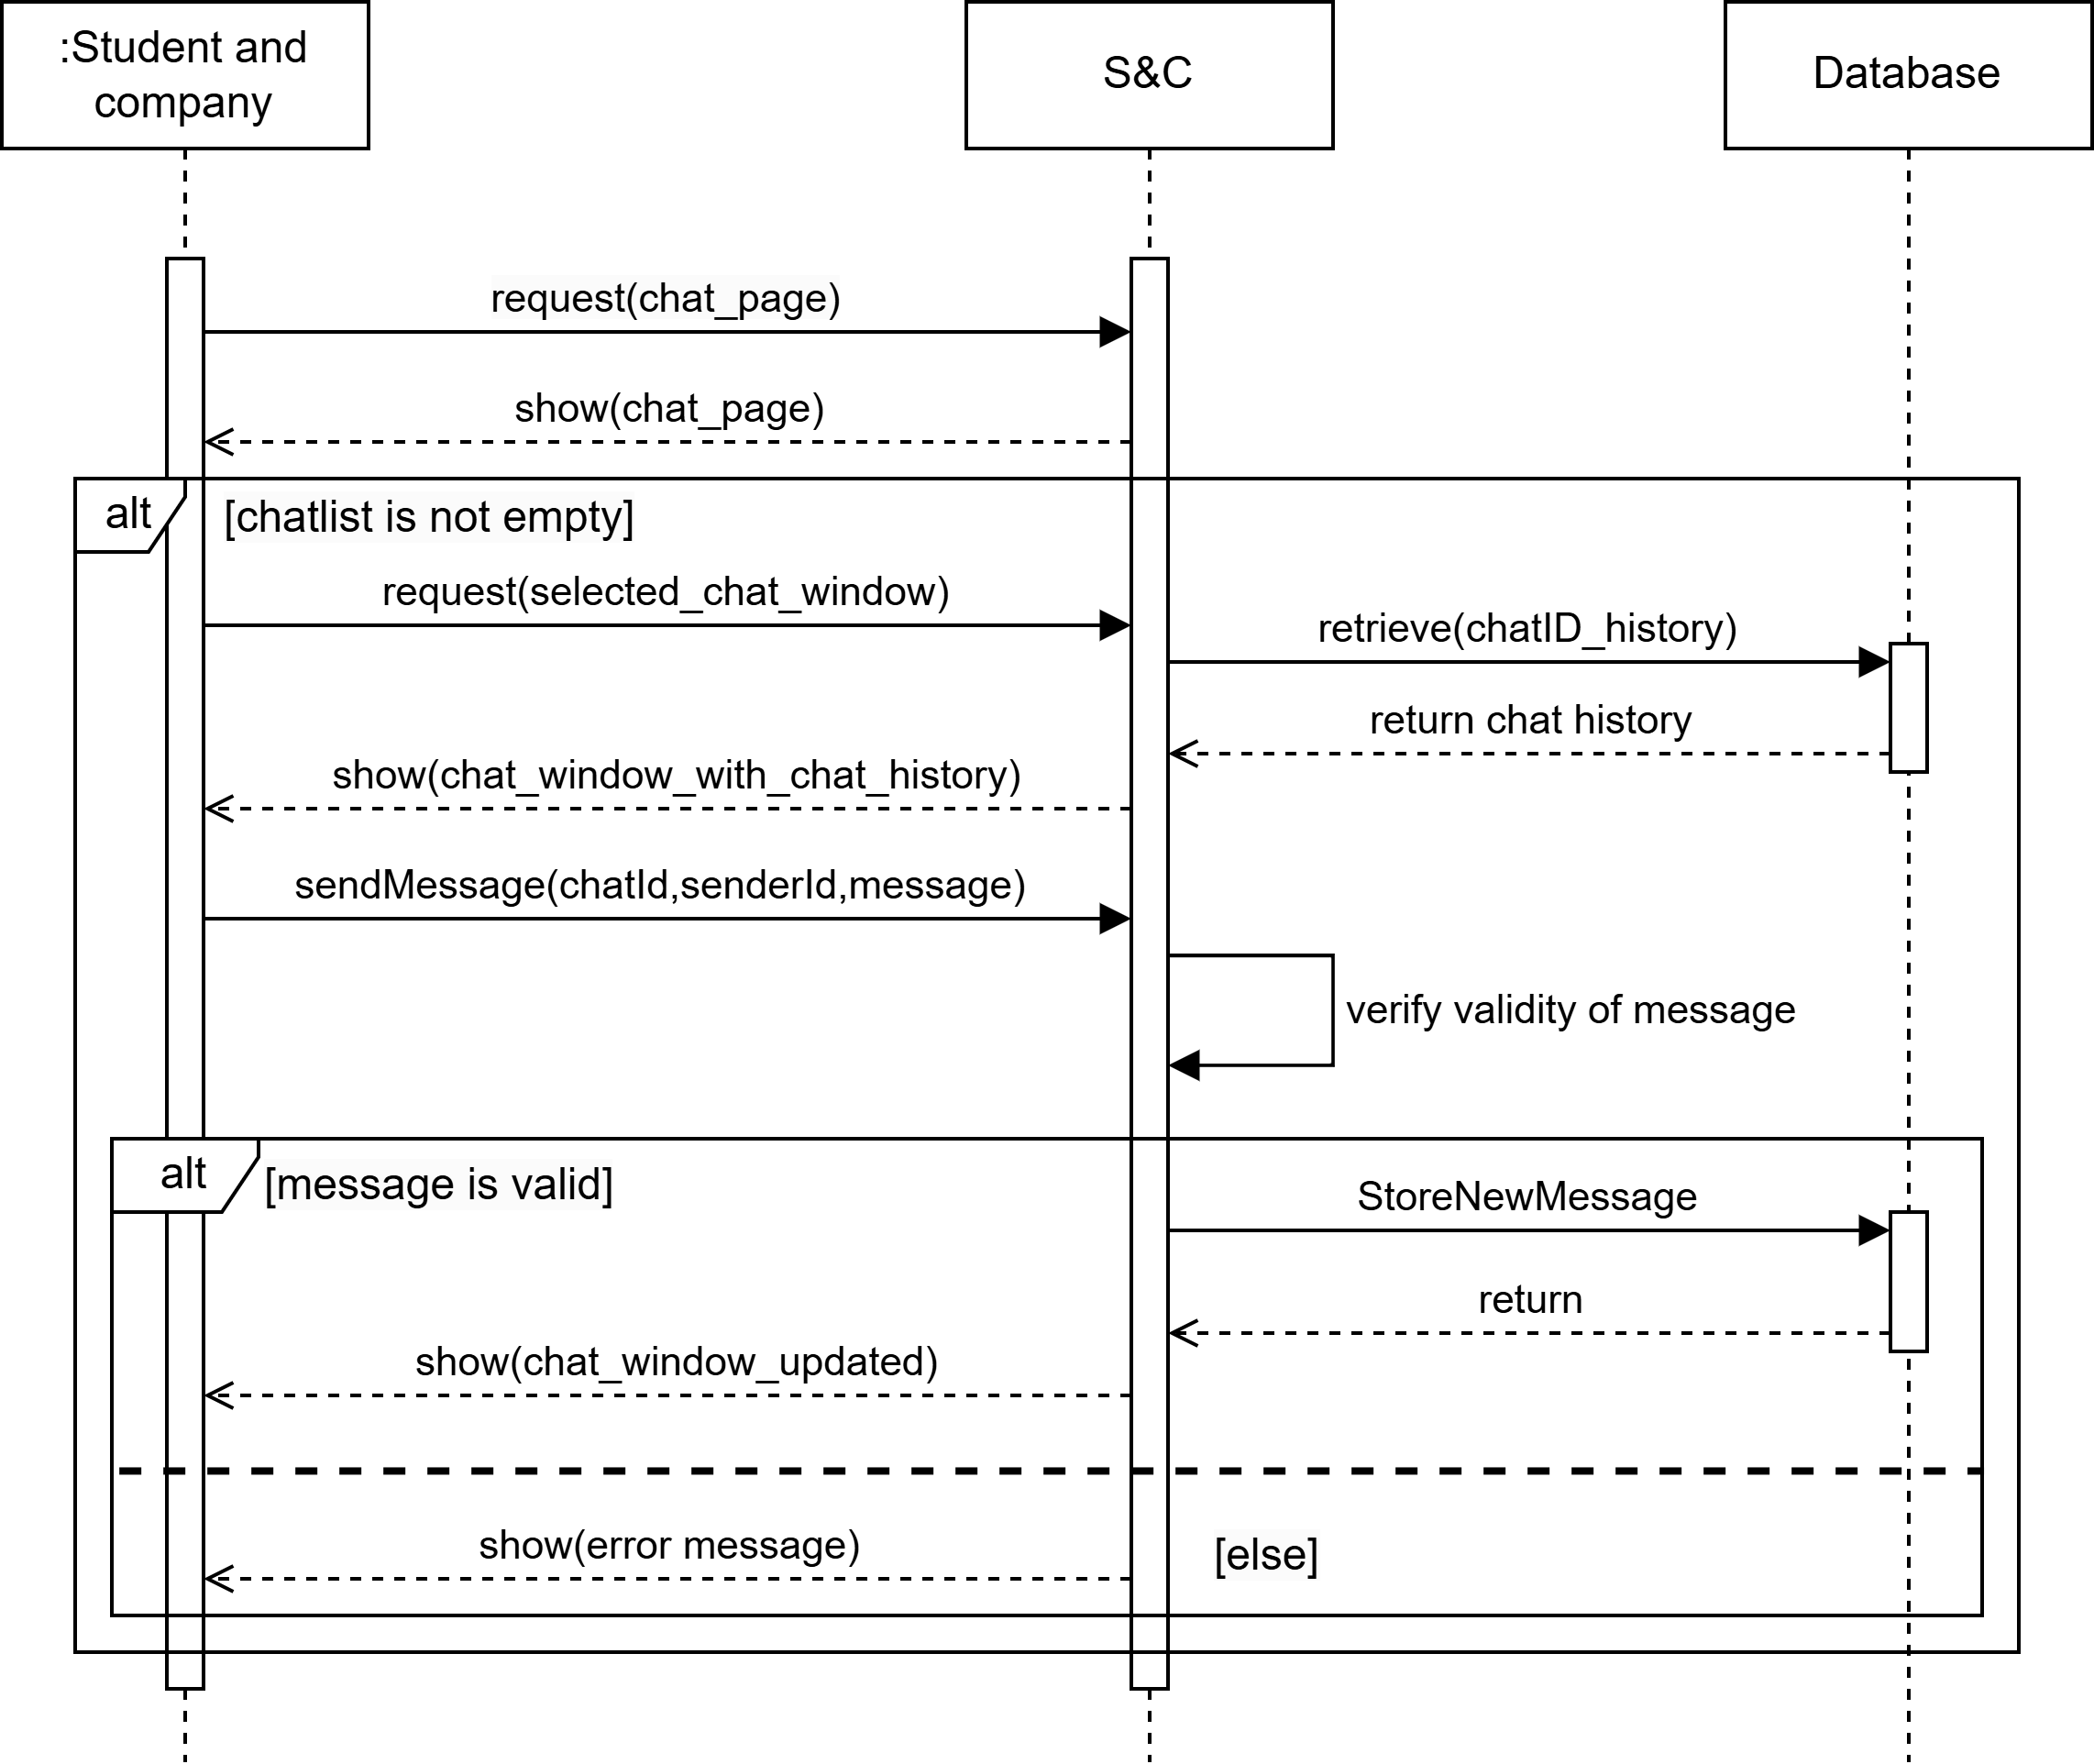
\includegraphics[width=0.75\textwidth]{Images/Sequence_Diagrams/chatting_SD.png}
    \caption{Student or Company chats with each other Sequence Diagram}
\end{figure}
% Use Case 14
\begin{figure}[H]
    \centering
    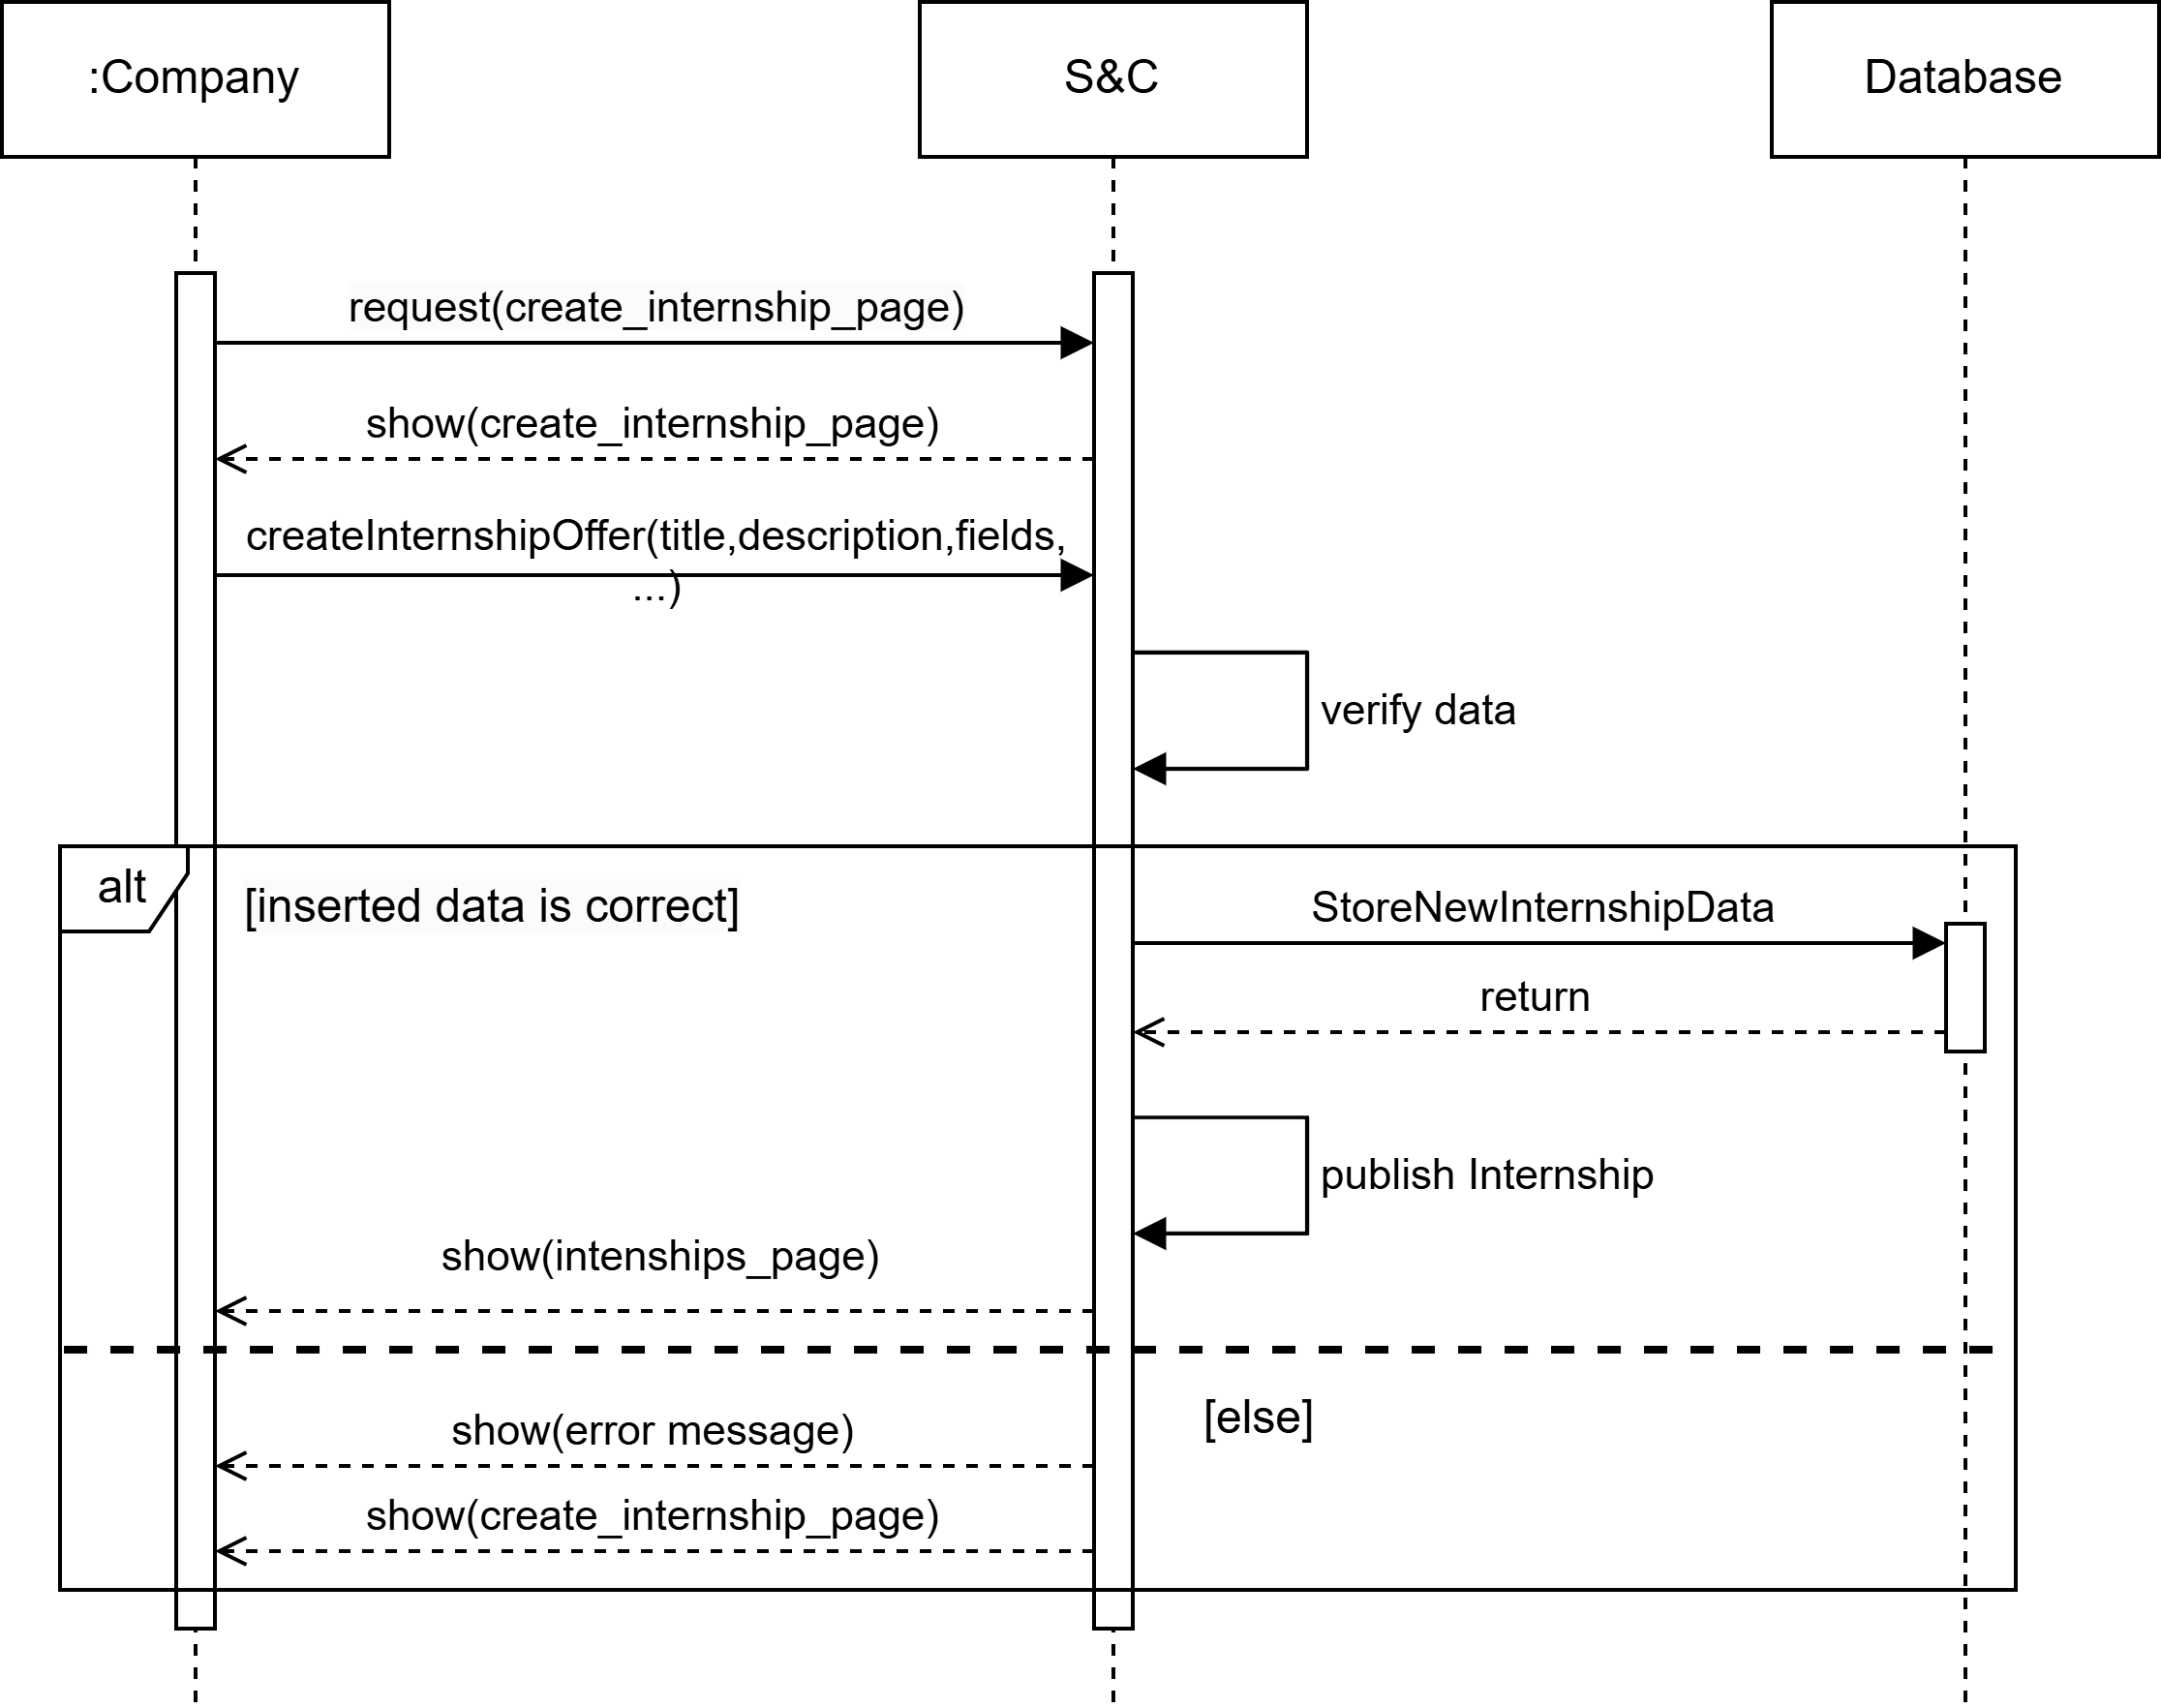
\includegraphics[width=0.75\textwidth]{Images/Sequence_Diagrams/createInt_SD.png}
    \caption{Company creates and publishes an internship Sequence Diagram}
\end{figure}
% Use Case 15
\begin{figure}[H]
    \centering
    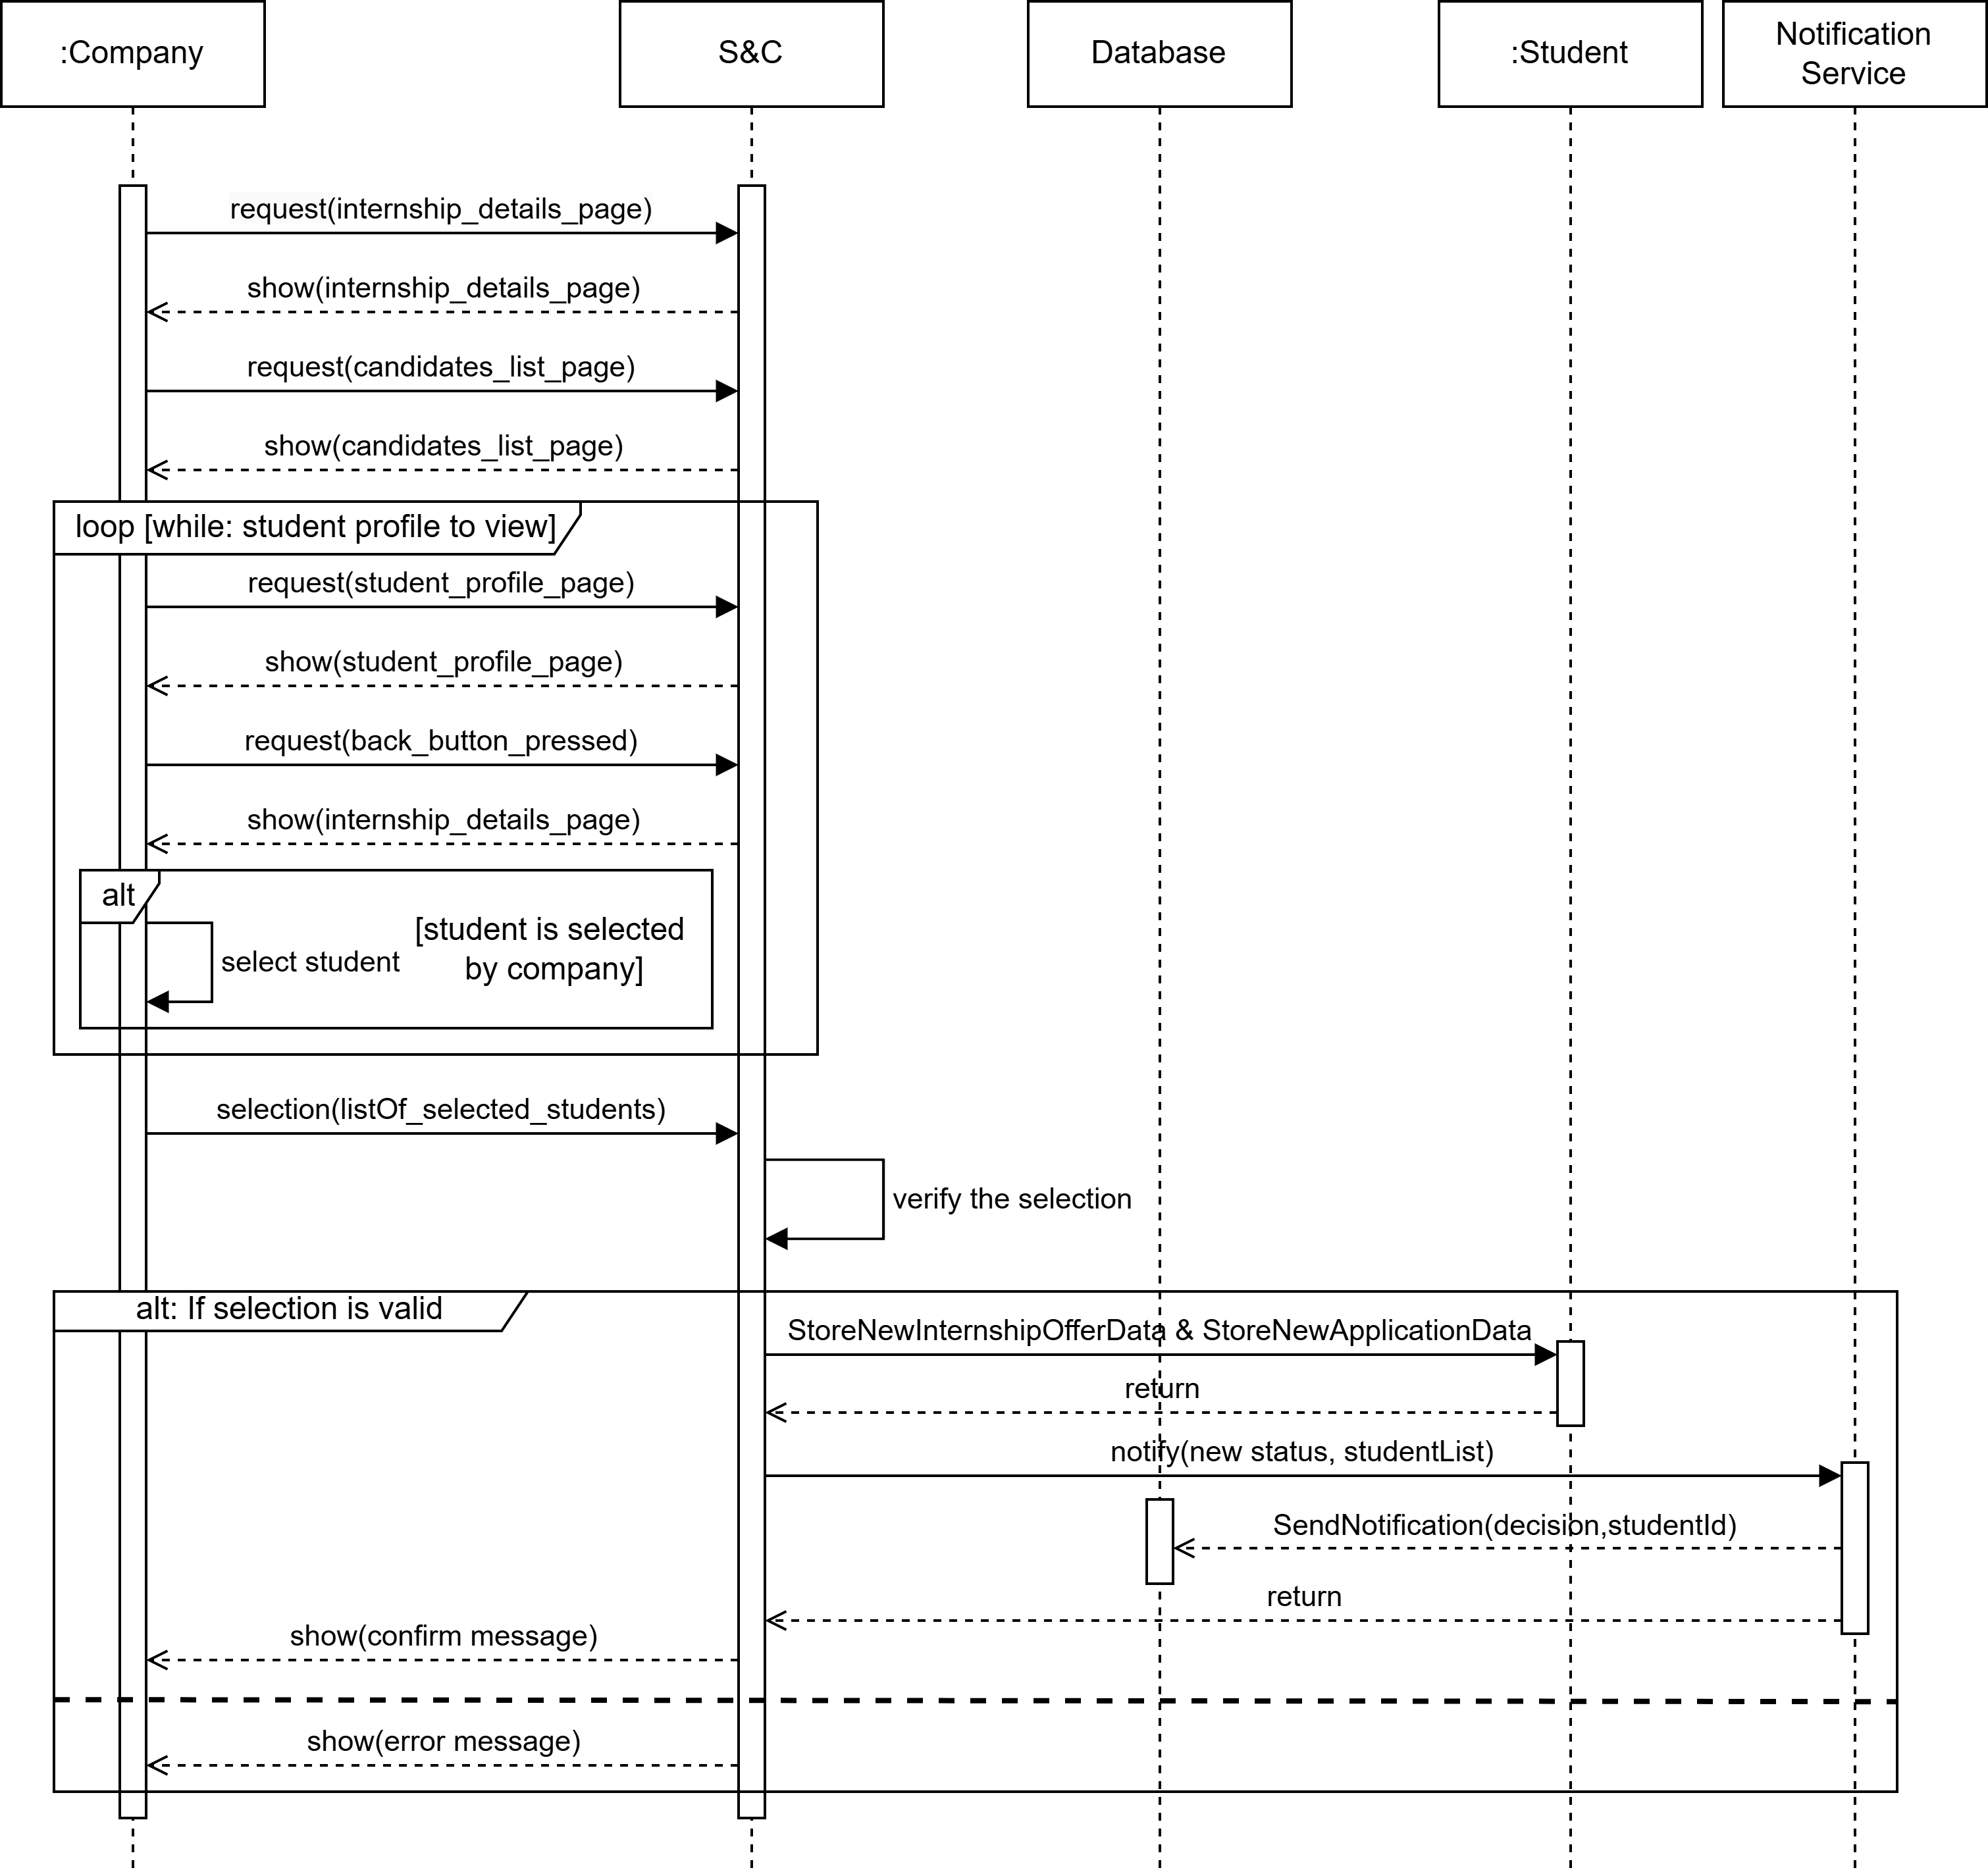
\includegraphics[width=1\textwidth]{Images/Sequence_Diagrams/select_SD.png}
    \caption{Company selects candidates Sequence Diagram}
\end{figure}
% Use Case 16
\begin{figure}[H]
    \centering
    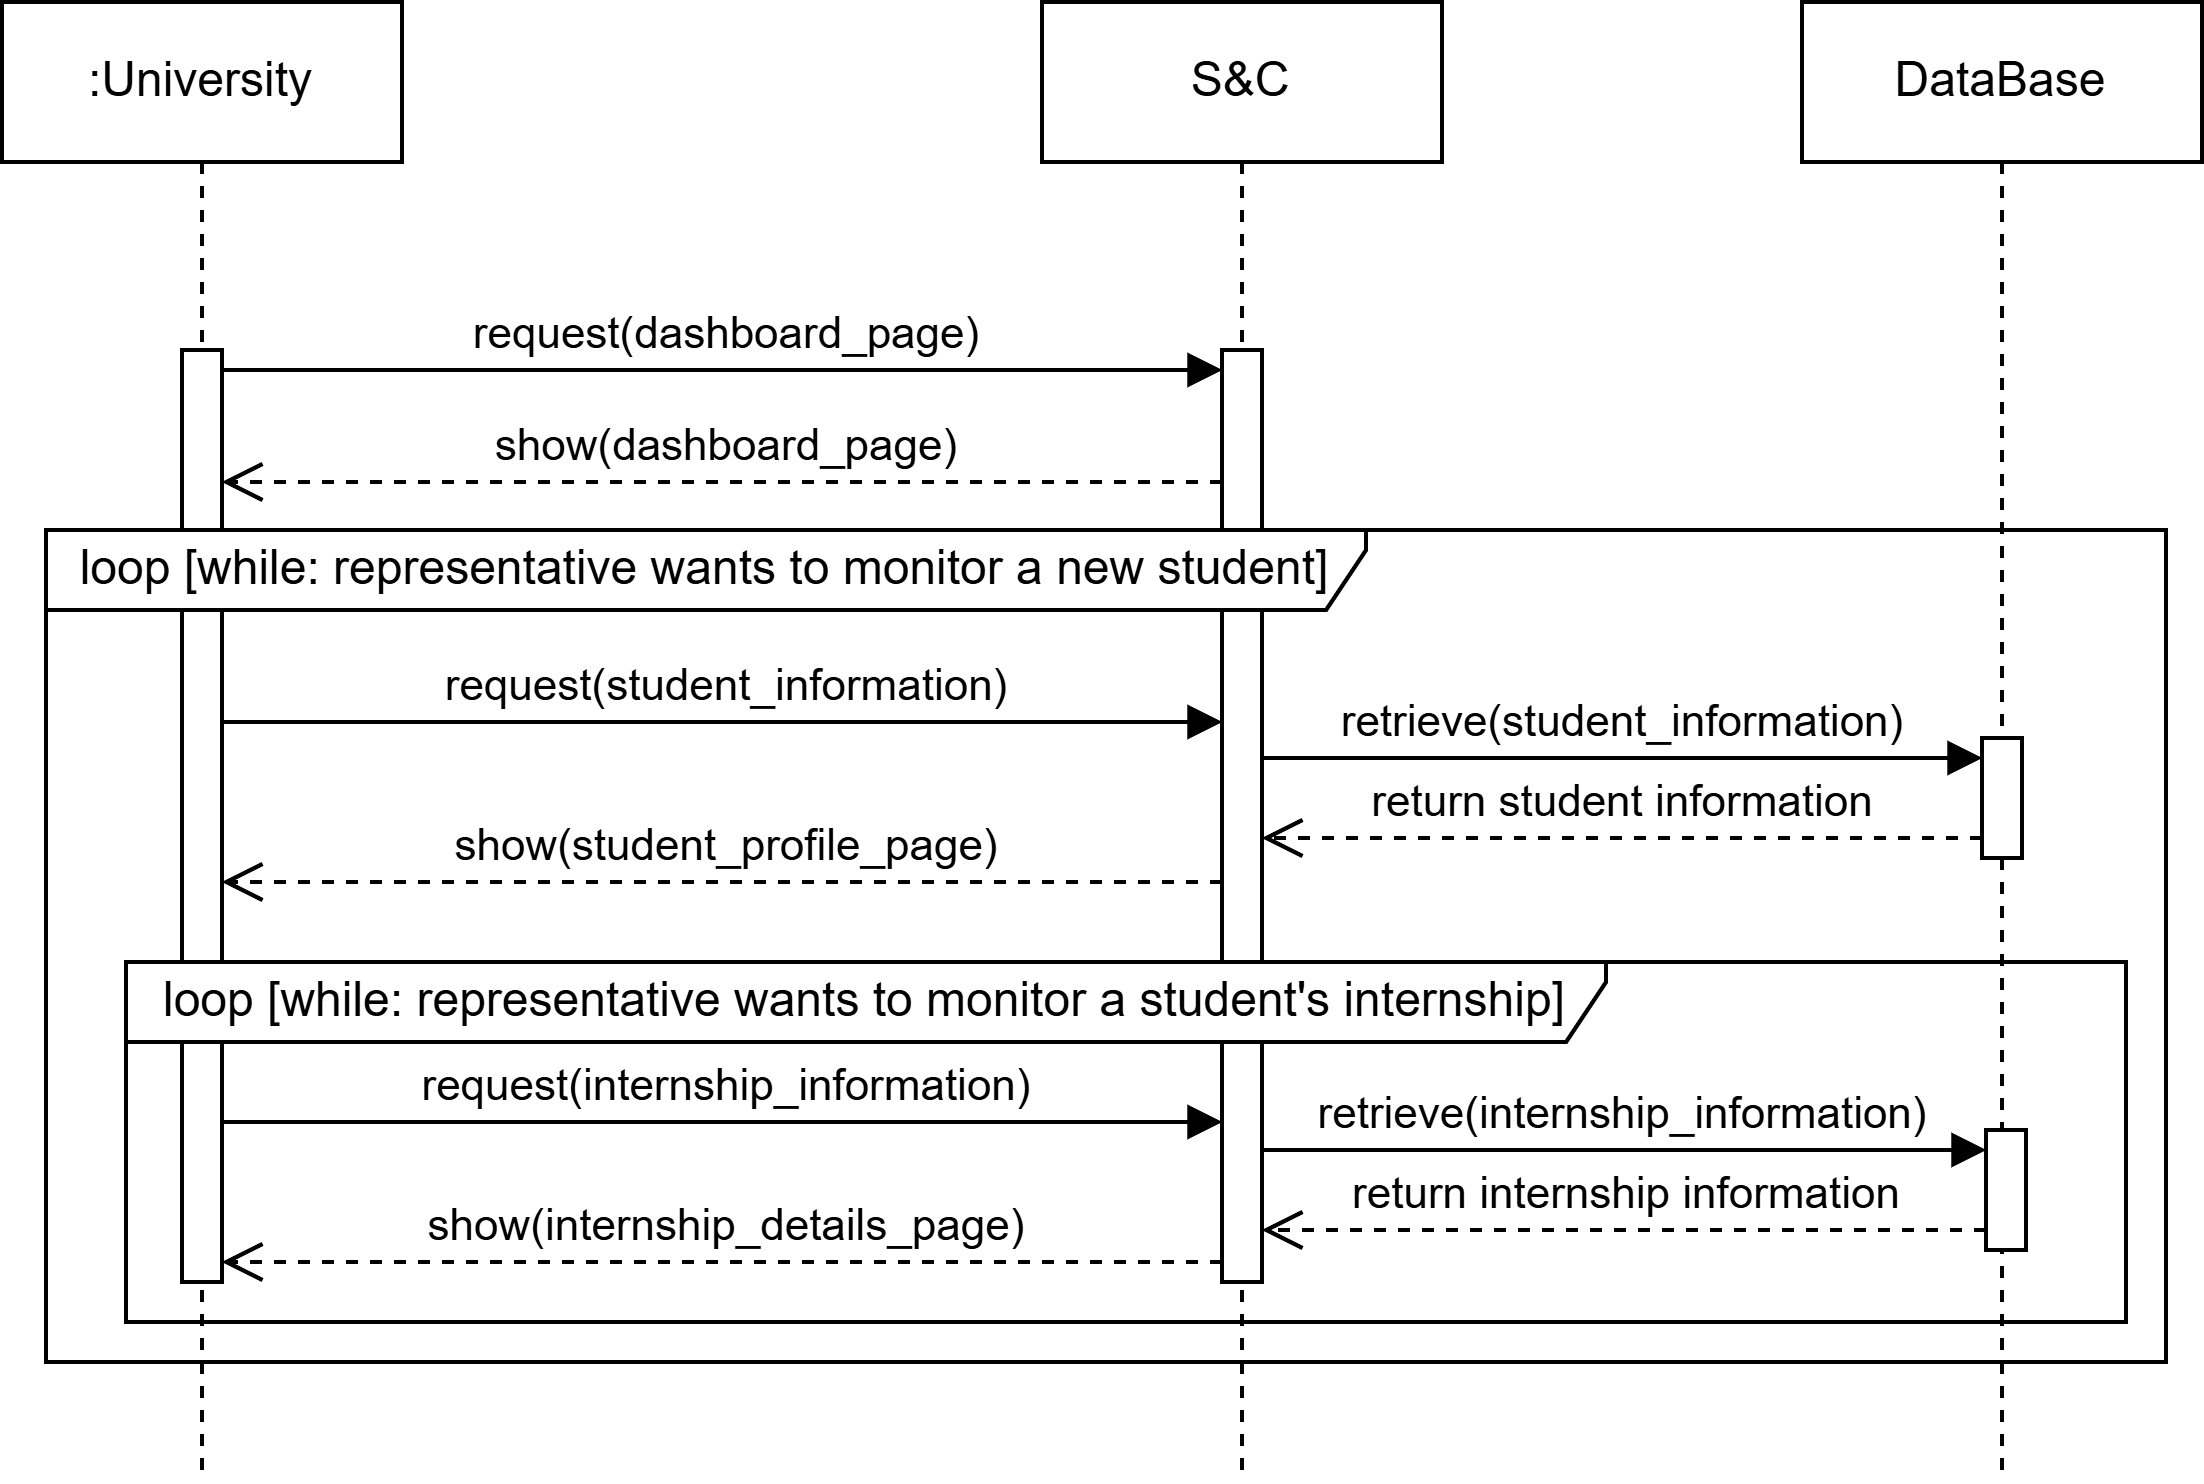
\includegraphics[width=0.70\textwidth]{Images/Sequence_Diagrams/monitor_SD.png}
    \caption{University monitors the internship processes of students Sequence Diagram}
\end{figure}


\subsection{Traceability Matrix}
Mapping the requirements to the use cases using the following matrix:

Note: \textit{Some requirements are mapped to multiple use cases because they relate to multiple functionalities.
However, in the matrix, we show only the one use case that is most relevant to the requirement.}

\begin{longtable}{|c|c|c|c|}
    \hline
    % Header row
    \textbf{Raw ID} & \textbf{Req. ID} & \textbf{Goal ID} & \textbf{Principal Use Case} \T\B \\
    \hline \hline
    \endfirsthead%
    
    \hline
    % Header row for subsequent pages
    \textbf{Raw ID} & \textbf{Req. ID} & \textbf{Goal ID} & \textbf{Principal Use Case} \T\B \\
    \hline \hline
    \endhead%
    
    \hline
    % Footer row for all pages except the last
    \multicolumn{3}{r}{\textit{Continued on next page}} \\
    \endfoot%
    
    \hline
    % Footer row for the last page
    \endlastfoot%
    % Table body
        \hline \hline
        \textbf{1} & R1 & G1 & U1.Register to S\&C   \T\B \\
        \hline
        \textbf{2} & R2 & G1 & U2.Login to S\&C  \T\B \\
        \hline
        \textbf{3} & R3 & G2 & U5.Upload CV  \T\B \\
        \hline
        \textbf{4} & R4 & G3 & U6.Search internship  \T\B \\
        \hline
        \textbf{5} & R5 & G4 & U14.Create and Publish Internship  \T\B \\
        \hline
        \textbf{6} & R6 & G4 & U14.Create and Publish Internship  \T\B \\
        \hline
        \textbf{7} & R7 & G4 & U14.Create and Publish Internship  \T\B \\
        \hline
        \textbf{8} & R8 & G5 & U15.Select Candidates  \T\B \\
        \hline
        \textbf{9} & R9 & G5 & U4. View recommendation  \T\B \\
        \hline
        \textbf{10} & R10 & G5 & U10.Send interview results  \T\B \\
        \hline
        \textbf{11} & R11 & G5 & U15.Select Candidates  \T\B \\
        \hline
        \textbf{12} & R12 & G5 & U11.Accept/reject offer  \T\B \\
        \hline
        \textbf{13} & R13 & G5, G6 & U4.View recommendation  \T\B \\
        \hline
        \textbf{14} & R14 & G5 & U15.Select Candidates  \T\B \\
        \hline
        \textbf{15} & R15 & G5 & U11.Accept/reject offer  \T\B \\
        \hline
        \textbf{16} & R16 & G5 & U11.Accept/reject offer  \T\B \\
        \hline
        \textbf{17} & R17 & G5 & U13.Chatting  \T\B \\
        \hline
        \textbf{18} & R18 & G5, G6 & U4.View recommendation  \T\B \\
        \hline
        \textbf{19} & R19 & G6 & U4.View recommendation  \T\B \\
        \hline
        \textbf{20} & R20 & G7 & U7.Apply internship  \T\B \\
        \hline
        \textbf{21} & R21 & G3, G7 & U6.Search internship \T\B \\
        \hline
        \textbf{22} & R22 & G8 & U15.Select Candidates  \T\B \\
        \hline
        \textbf{23} & R23 & G8 & U15.Select Candidates  \T\B \\
        \hline
        \textbf{24} & R24 & G8 & U8.Create interview\T\B \\
        \hline
        \textbf{25} & R25 & G9 & U9.Respond to interview questionnaire \T\B \\
        \hline
        \textbf{26} & R26 & G10 & U10.Send interview results  \T\B \\
        \hline
        \textbf{27} & R27 & G10 & U12.Send interview results  \T\B \\
        \hline
        \textbf{37} & R28 & G11 & U14.Accept/reject offer  \T\B \\
        \hline
        \textbf{29} & R29 & G11 & U14.Accept/reject offer \T\B \\
        \hline
        \textbf{30} & R30 & G12 & U12.Write feedback and complaints  \T\B \\
        \hline
        \textbf{31} & R31 & G12 & U12.Write feedback and complaints \T\B \\
        \hline
        \textbf{32} & R32 & G13 & U13.Chatting  \T\B \\
        \hline
        \textbf{33} & R33 & G14 & U16.Monitor internship of students  \T\B \\
        \hline
        \textbf{34} & R34 & G14 & U16.Monitor internship of students  \T\B \\
        \hline
        \textbf{35} & R35 & G14 & U3.See profile information  \T\B \\
        \hline
        \textbf{36} & R36 & G2 & U5.Upload CV \T\B \\
        \hline
        \textbf{37} & R37 & G5, G12 & U1.Register to S\&C  \T\B \\
        \hline
    \end{longtable}


\section{Performance Requirements}
\begin{itemize}
    \item \textbf{Concurrent access of users and resource utilization:} A platform like Students\&Companies is expected to have a large
    number of users, so it must be able to handle multiple requests simultaneously. By searching online for platforms that offer similar
    services we have found that a good estimate for the number of concurrent users that the platform should be able to manage is roughly
    a few thousands, peaking at a few tens of thousands during peak internship publishing periods (like at the end of universities semesters). \\
    The platform should be able to optimize the resource utilization to ensure that the system can handle the load without any performance
    issues. This includes optimizing the database queries, caching data, and using load balancing techniques to distribute the load across
    multiple servers.
    
    \item \textbf{Data processing and storage:} The system should be able to process and store a large amount of data efficiently. From 
    what we were able to find online, similar platforms estimate that the number of registered users can reach a few hundreds of thousands,
    and the number of internships published can reach a few tens of thousands. For this reason, the database should be able to easily handle
    a few terabytes of data. \\
    The platform should also be able to process data quickly, especially when performing statistical analyses in order to generate recommendations 
    for students and companies. This includes optimizing the queries made by recommendation algorithm to ensure that it can provide 
    recommendations in real-time.

    \item \textbf{Time of Response:} From the users' perspective, the system should be responsive, meaning the response to any of his request 
    should appear instantly. In order to achieve this, the response time for most operations, such as loading a page, submitting an application, 
    or performing a search, should be at most a few seconds during peak usage and in the domain of milliseconds in normal conditions. \\
    Particular attention should be given to the recommendation algorithm, which should be able to provide recommendations in real-time,
    to the chat functionality, which should allow users to communicate in real-time, and to the notification system, who must ensure that
    updates are delivered to the user before relevant deadlines expire. \\
    The response time of other operations such as the ones that involve the mailing system cannot be guaranteed by S\&C.
\end{itemize}


\section{Design Constraints}

\subsection{Standards Compliance}
The platform should comply with the REST API standard in order to correctly process user inputs. \\
The system must be compliant with the European Union's General Data Protection Regulation (GDPR), which is a set of regulations that is designed
to protect the privacy and personal data of individuals within the European Union. This means that the platform must ensure that user data is
collected and processed in a lawful and transparent manner, and that users have the right to access, correct, and delete their data. \\
The platform should also comply with the Web Content Accessibility Guidelines (WCAG) to ensure that the platform is accessible to users with
disabilities. This includes providing multiple ways to navigate the platform, for example by showing alternative text for images. \\
Since the users accessing the platform could be from different countries and timezones, the platform should use a time standard like UTC to
ensure that all dates and times are consistent across different regions and that deadlines can be communicated and handled without ambiguity.

\subsection{Hardware Limitations}
The platform is a web-based application, so it should be able to run on any device with an internet connection and a compatible web browser. 
Furthermore, it should not require high level or specific hardware.

\subsection{Any Other Constraint}
S\&C is intended for students, companies and universities only, so the platform should not be accessible to users who do not belong to these
categories. \\
The target of the platform is the European market. Since users may speak different languages, it should be designed completely in English, as 
it is the most widely spoken language and is commonly used in the business and academic world.


\section{Software System Attributes}
\subsection{Reliability}
The platform should be reliable and ensure that the data is always available and consistent. Particular attention should be given to the
recommendation algorithm, which should be programmed with the utmost care so that it is always working properly and recommendations are always accurate. 
This is because uninteresting and unfit recommendations could lead to a decrease in the platform's popularity and a loss of users. \\
The system should also be able to cope with partial failures through replication and recover from failures quickly and without data loss. 
This includes implementing regular backups of the database and the state.

\subsection{Availability}
The system should have a required uptime of at least 99.8\%, which means that the platform should be available 99.8\% of the time. 
This is equivalent to a downtime of less than 18 hours per year. To achieve this, the platform should be designed with fault tolerance 
in mind to ensure that the system can handle failures without affecting the availability. \\
During the downtime period, a maintenance page should be displayed to inform users that the platform is being updated or is experiencing
technical difficulties and is currently unavailable. In order to avoid the expiration of a deadline during the downtime, planned maintenance 
should be scheduled during off-peak hours, such as late at night or early in the morning.

\subsection{Security}
In order to guarantee a secure system, the platform should control the access rights of the users, ensuring both authentication, meaning that 
the identity of users that attempt to login must be verified, and authorization, meaning that the permission of users to perform specific actions
must be verified. As an example, a student should not be allowed to create an internship. \\
To comply with the GDPR, the platform should encrypt all sensitive data, such as passwords and personal information, using secure communication protocols, 
like HTTPS, TLS, and specific algorithms.

\subsection{Scalability}
The system should be designed to be scalable, meaning that it shouldn't sacrifice performance as the number of concurrent users and stored data grows.
This includes the ability to scale horizontally by adding more servers in order to distribute the load and the ability to scale vertically by upgrading 
the backend hardware to increase the system's capacity. \\
In particular, the recommendation algorithm must be able to scale well. It should be optimized to handle a larger number of users and data, and ensure
that it can provide recommendations in real-time.

\subsection{Maintainability}
The platform should be easy to maintain and update. This includes writing clean, understandable and well-documented code, using version control systems 
to track changes, and following best practices for software development, like writing unit tests and using continuous integration and deployment tools. \\
The platform should also be designed to be modular, meaning that different components should be decoupled and independent from each other, so that
they can be updated or replaced by different development teams without affecting the rest of the system.

\subsection{Portability}
The system should be compatible with any kind of device that has an internet connection and a compatible web browser. This includes desktops, laptops,
tablets, and smartphones.
